\chapter{APPENDIX: $Z\gamma$ Check}
\label{sec:ZgCheck}

For the $Z\gamma$ check, the same procedures we use for the $W\gamma$ measurement, we also use for the $Z\gamma$ measurement except those that are not applicable. Figure~\ref{fig:DATAvsMC_Zg} shows the data vs MC distribution of $Z\gamma$-selected samples. The selected sample mostly consists of $Z\gamma$ signal event and DY+jets background. DY+jets background is a source of jets$\rightarrow\gamma$ background and is estimated the same way as it is done for our nominal $W\gamma$ measurement.  

The templates are derived from $Z\gamma\rightarrow\mu\mu\gamma$ sample, therefore, the $Z\gamma$ check in the muon channel is not a valid physics measurement but a closure check because the templates for the jets$\rightarrow\gamma$ background estimation procedure are largely overlap with the fitted data. At the same time, the $Z\gamma$ check in the electron channel is a valid physics measurement. Fit results on data and pseudodata (MC mixtures) show good agreement for both channels (Fig.~\ref{fig:DDvsMC_Zg_Data_MUON}-\ref{fig:DDvsMC_Zg_MCclosure_ELECTRON}). The fit plots themselves are available in App.~\ref{sec:TemplateFitPlotsZGamma}-\ref{sec:TemplateFitPlotsMCclosure_ZGamma}.

Major systematic uncertainties are estimated the same way as it is done for $W\gamma$ measurement and are listed in Tab.~\ref{tab:systInPercent_MUON_ZGamma}-\ref{tab:systInPercent_ELECTRON_ZGamma}. Measured cross section values compared to the MC-based cross section are listed in the Tab.~\ref{tab:sc_mc_vs_meas_MUON_ZGamma}-\ref{tab:sc_mc_vs_meas_ELECTRON_ZGamma}. Figure~\ref{fig:CS_Zg} shows an agreement between muon and electron channels, agreement with the MC-based cross section and with the approved $Z\gamma$ measurement with CMS at $\sqrt{s}=8$~TeV~\cite{ref_Zg8TeV}.


\begin{figure}[htb]
  \begin{center}
   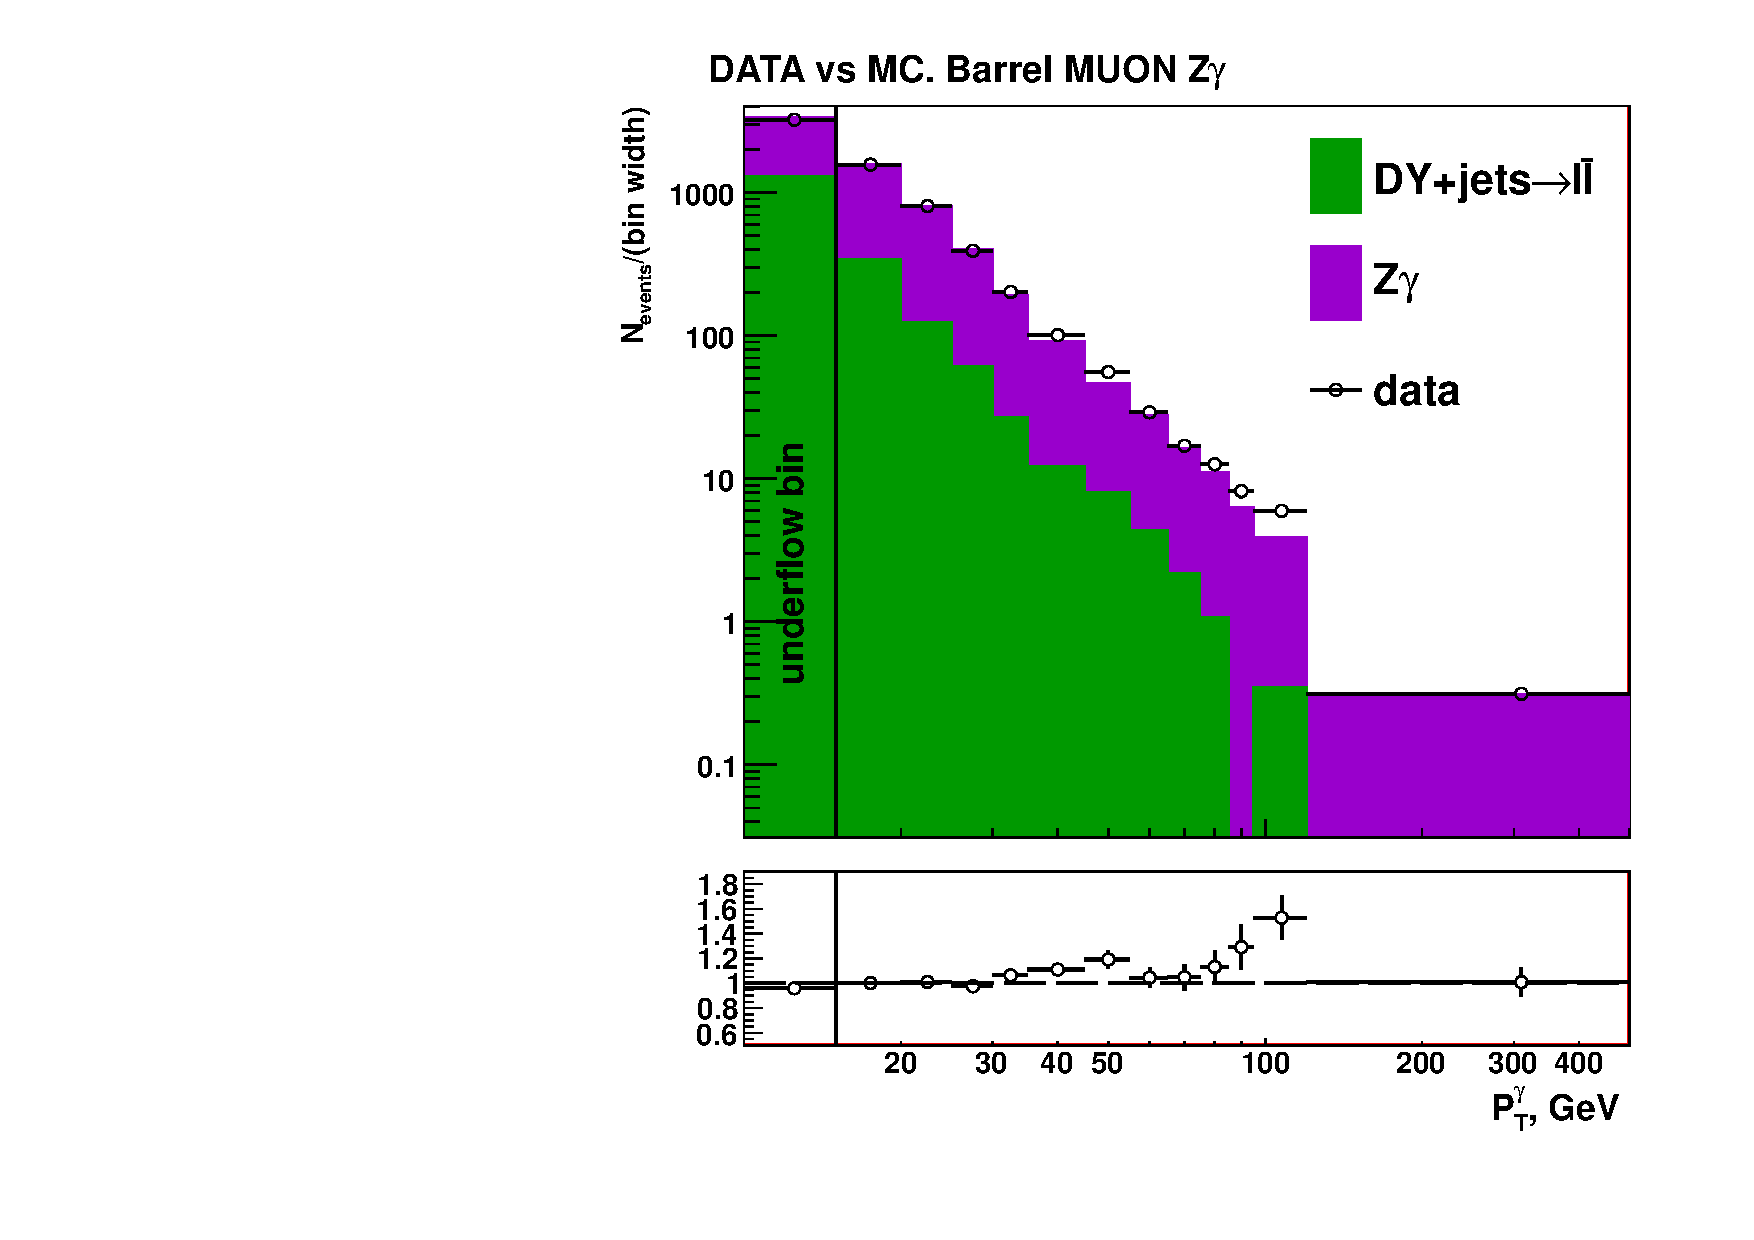
\includegraphics[width=0.45\textwidth]{../figs/figs_v11/MUON_ZGamma/PrepareYields/c_TotalDATAvsMC_Barrel__phoEt.pdf}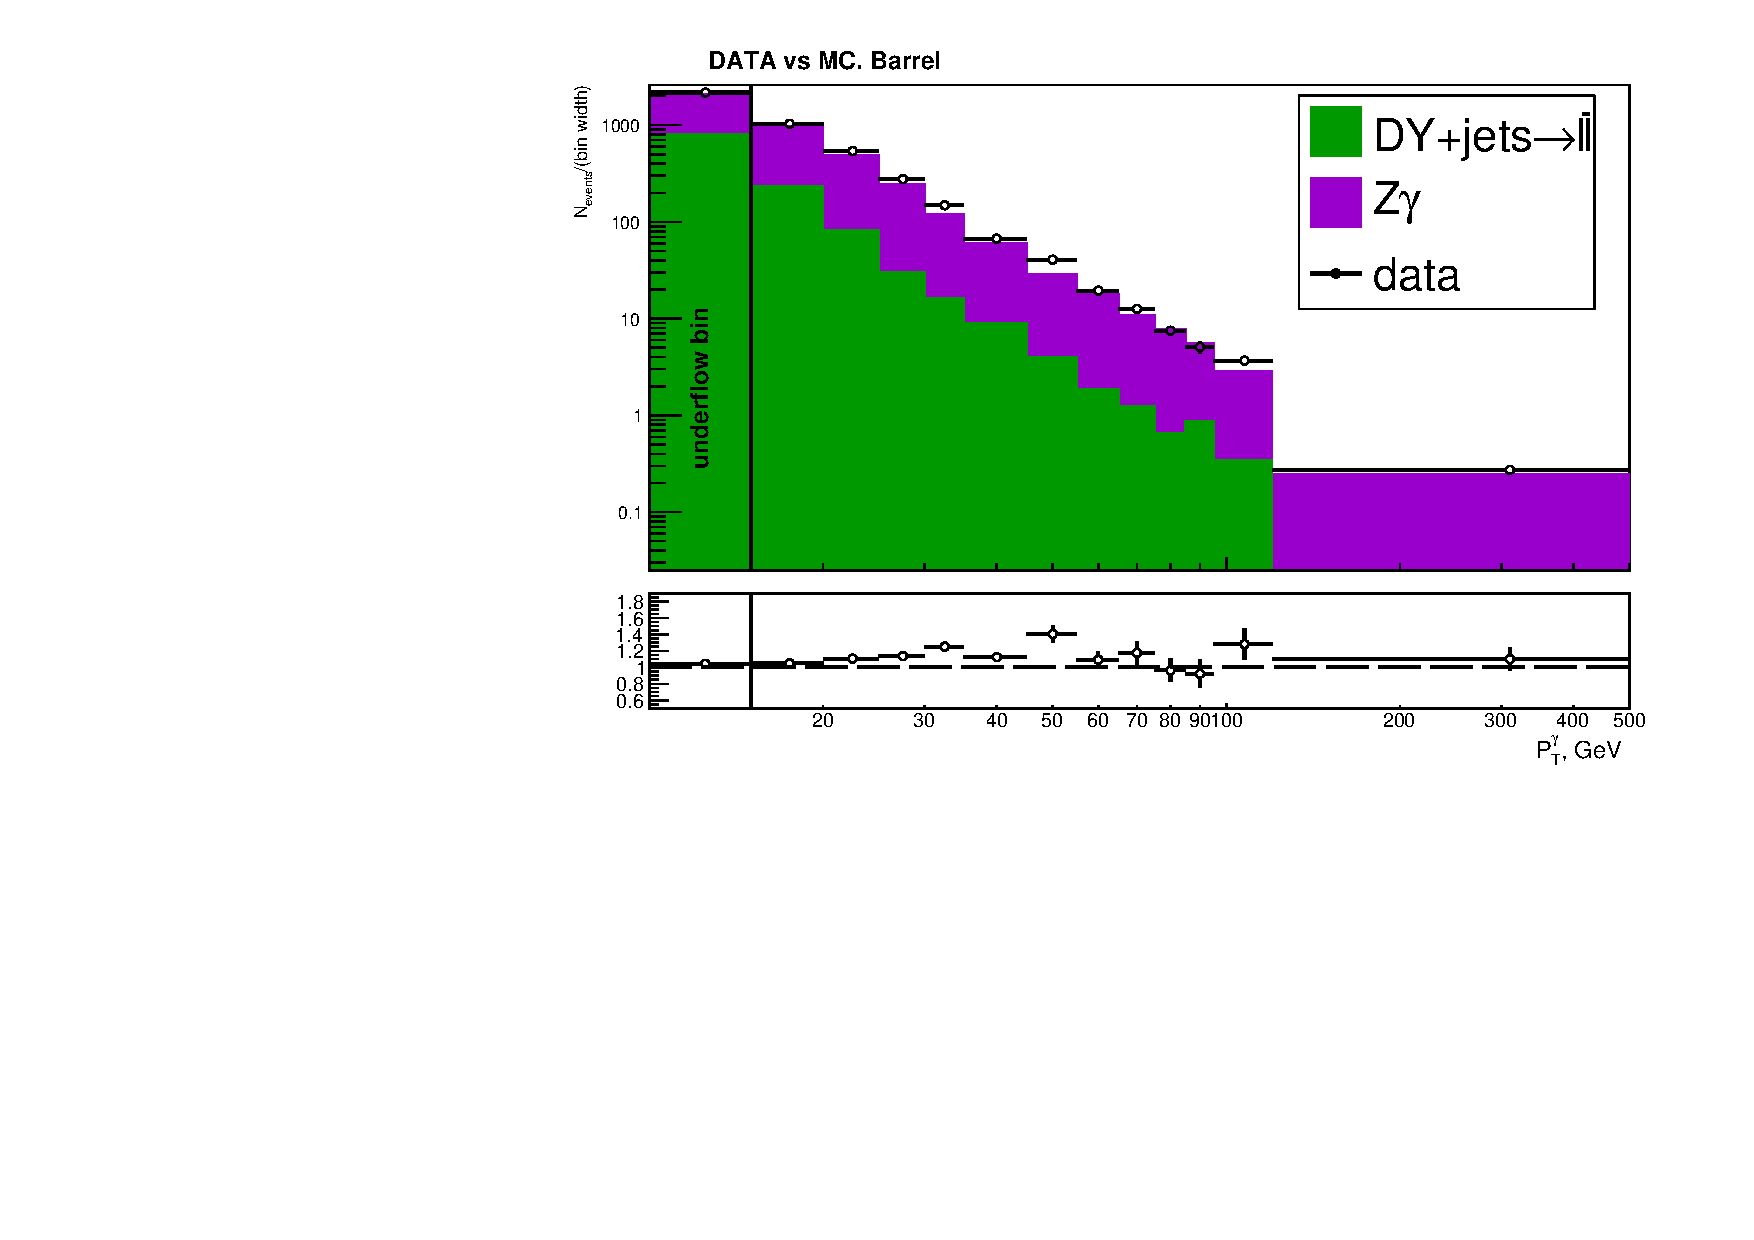
\includegraphics[width=0.45\textwidth]{../figs/figs_v11/ELECTRON_ZGamma/PrepareYields/c_TotalDATAvsMC_Barrel__phoEt.pdf}
   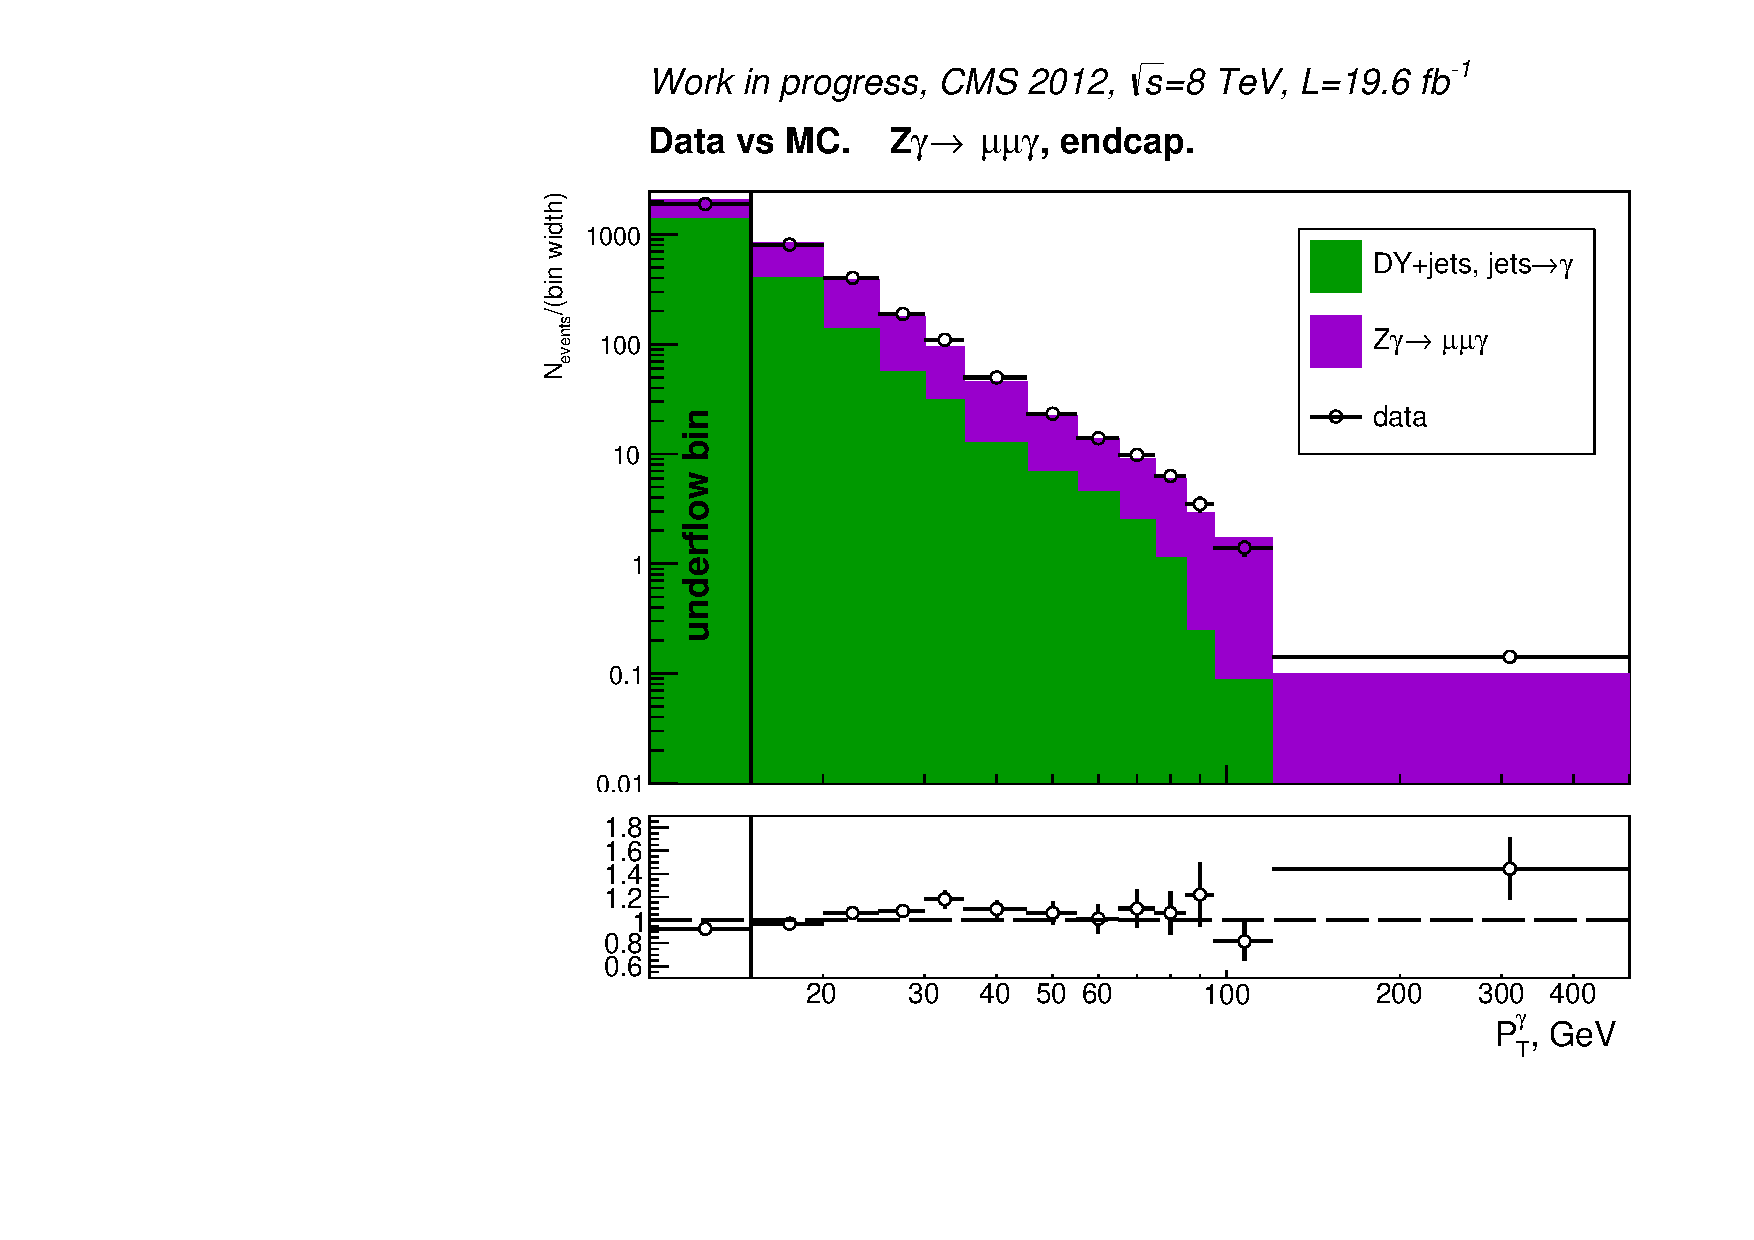
\includegraphics[width=0.45\textwidth]{../figs/figs_v11/MUON_ZGamma/PrepareYields/c_TotalDATAvsMC_Endcap__phoEt.pdf}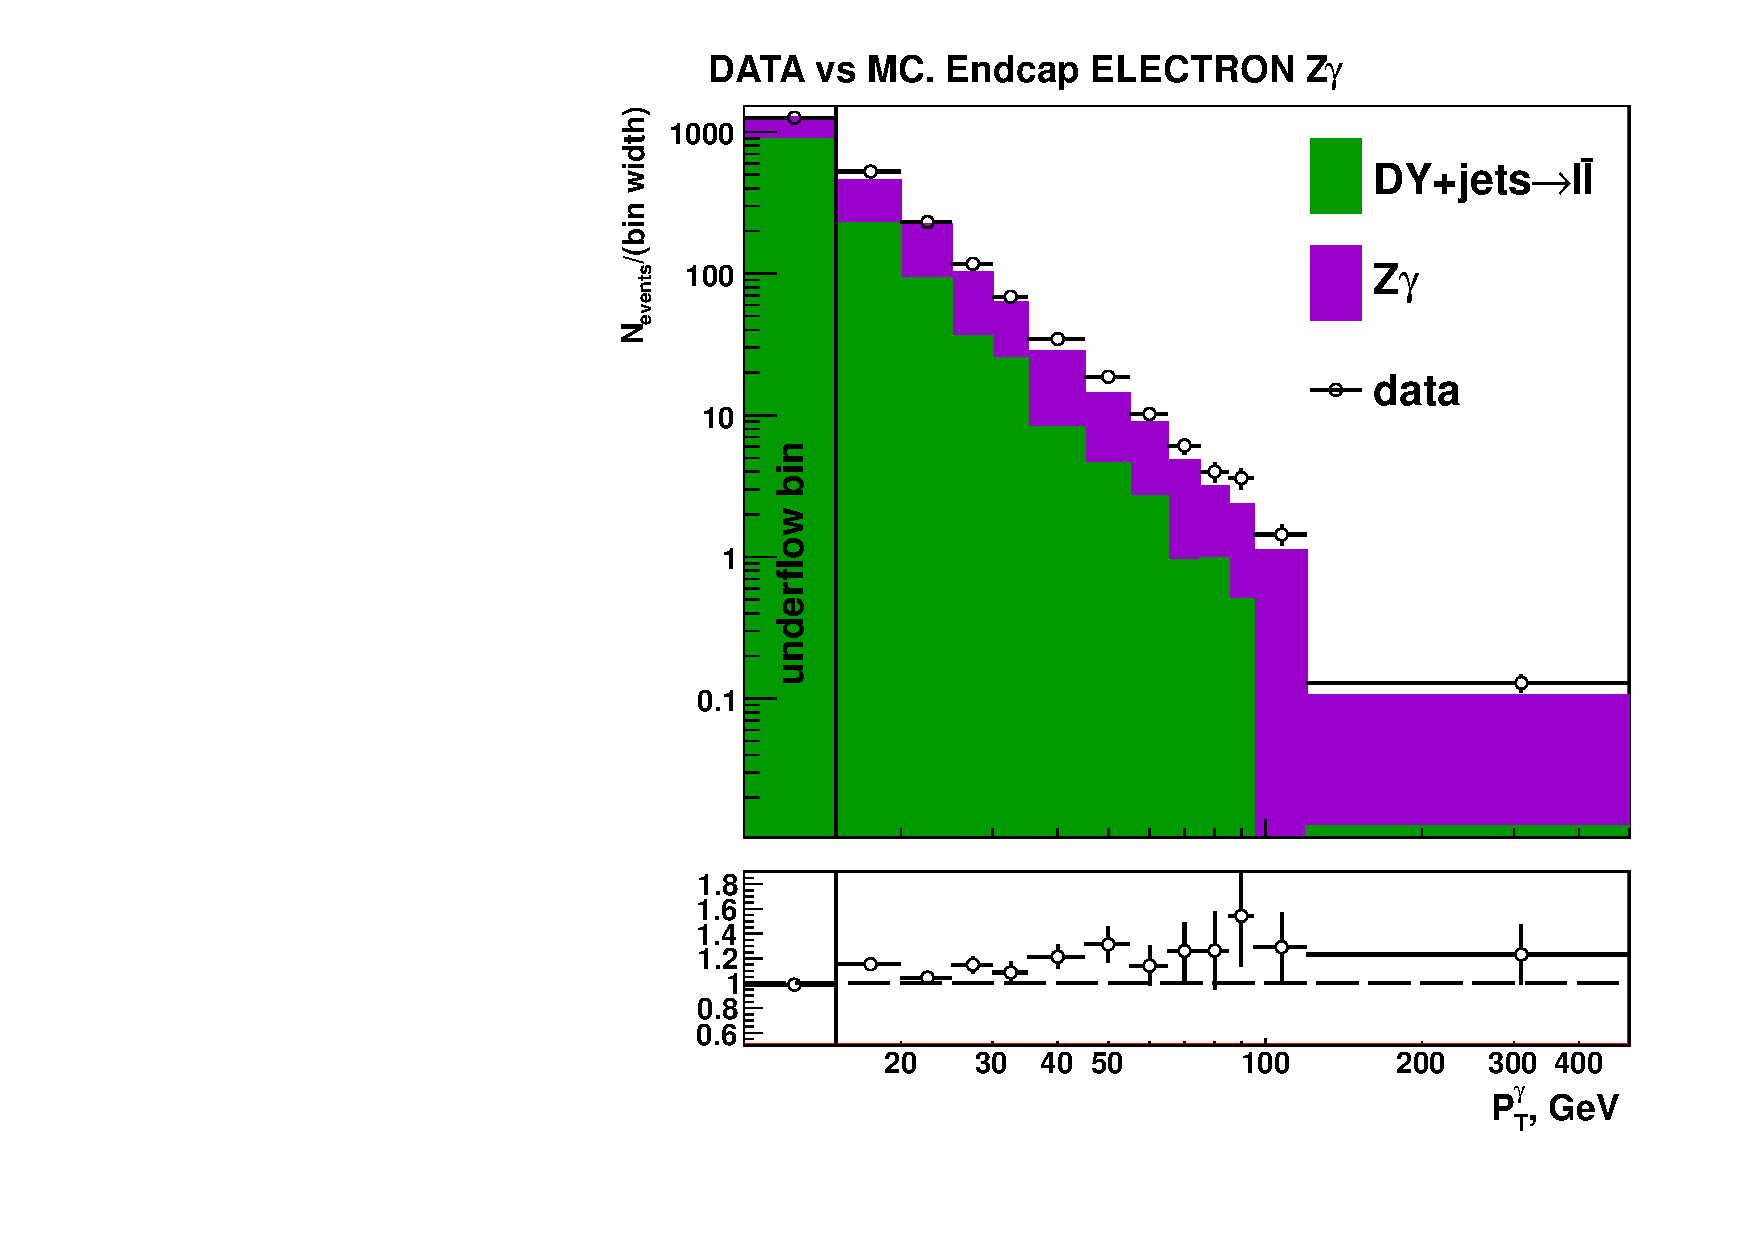
\includegraphics[width=0.45\textwidth]{../figs/figs_v11/ELECTRON_ZGamma/PrepareYields/c_TotalDATAvsMC_Endcap__phoEt.pdf}
  \caption{Data vs MC plots. Left column - muon channel, right column - electron channel. Top to bottom: barrel and endcap photons}
  \label{fig:DATAvsMC_Zg}
  \end{center}
\end{figure}

\begin{figure}[htb]
  \begin{center}
   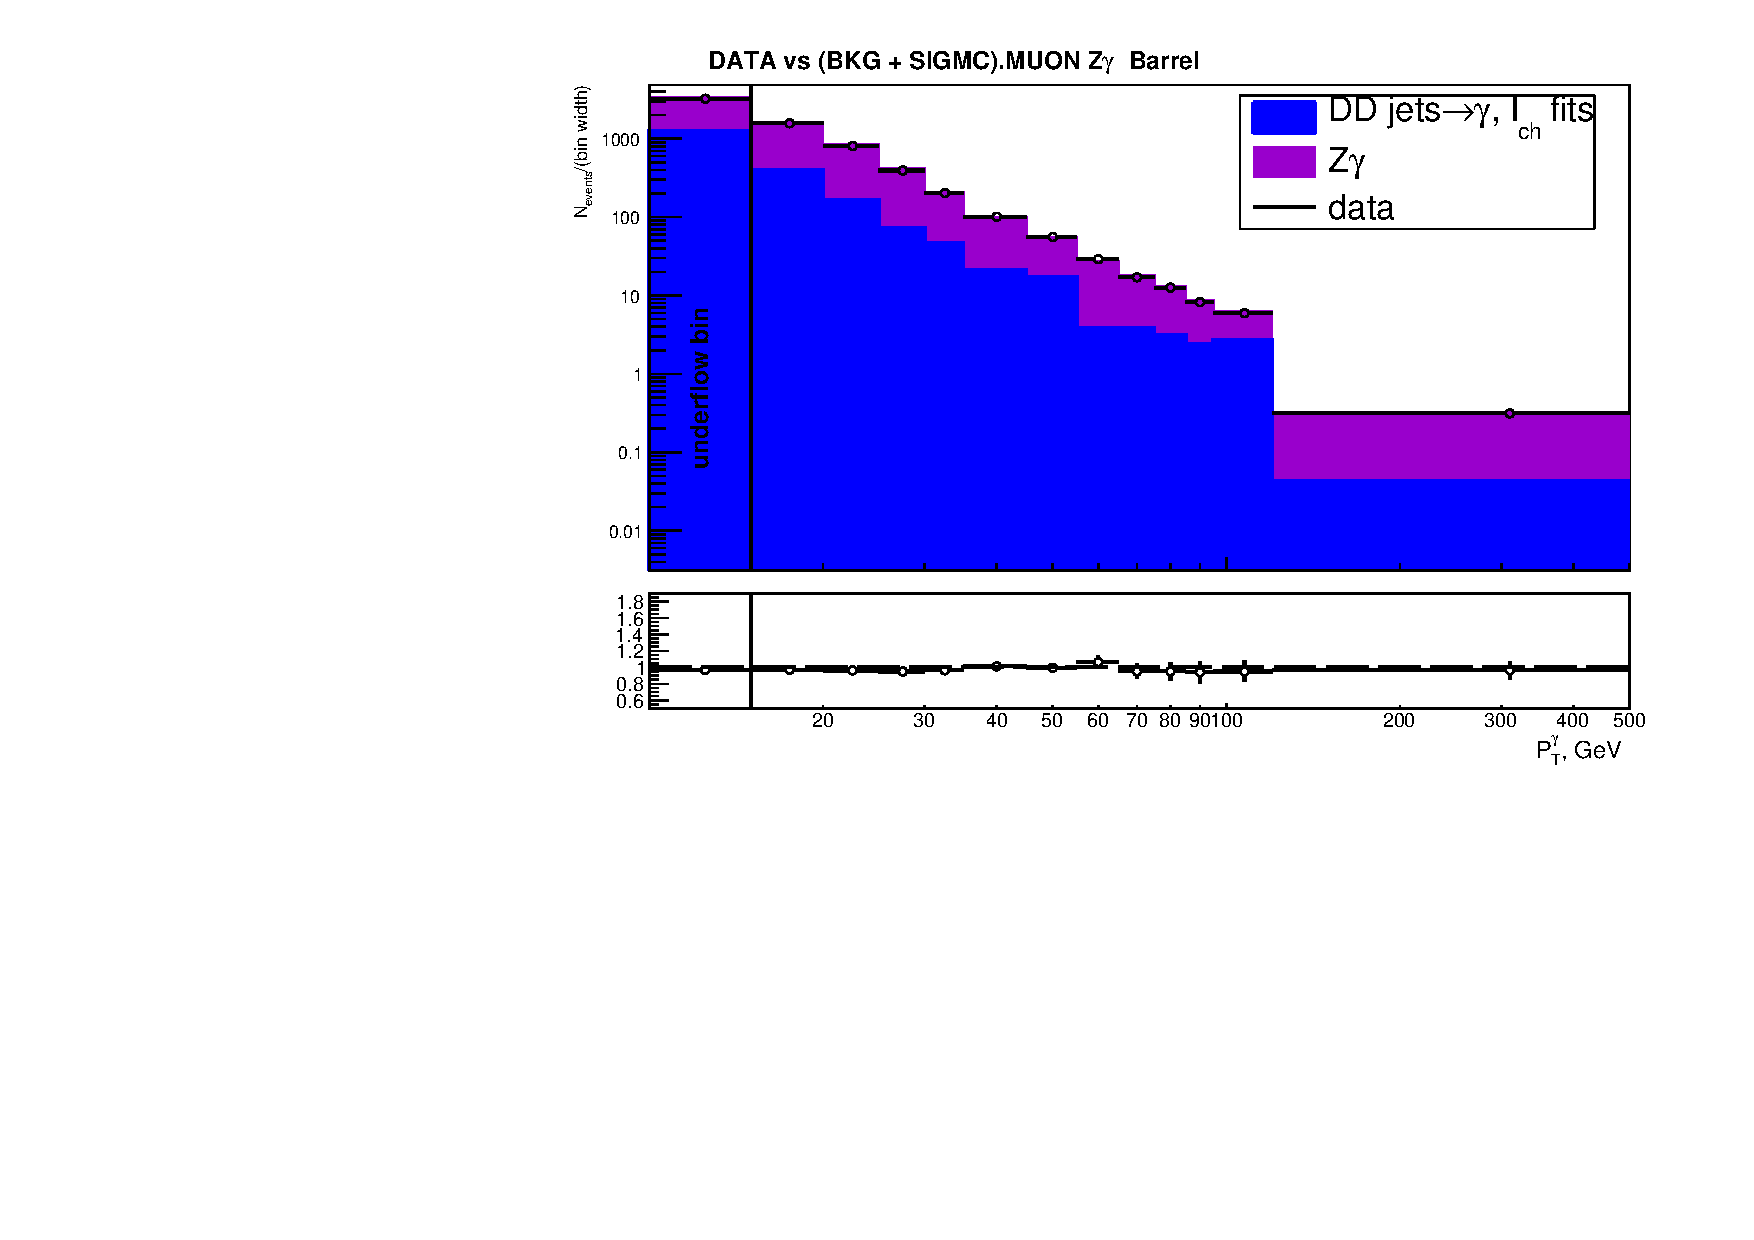
\includegraphics[width=0.45\textwidth]{../figs/figs_v11/MUON_ZGamma/PrepareYields/c_DATAvsBkgPlusSigMCc_MUON_ZGamma_TEMPL_CHISO_UNblind__Barrel__phoEt.pdf}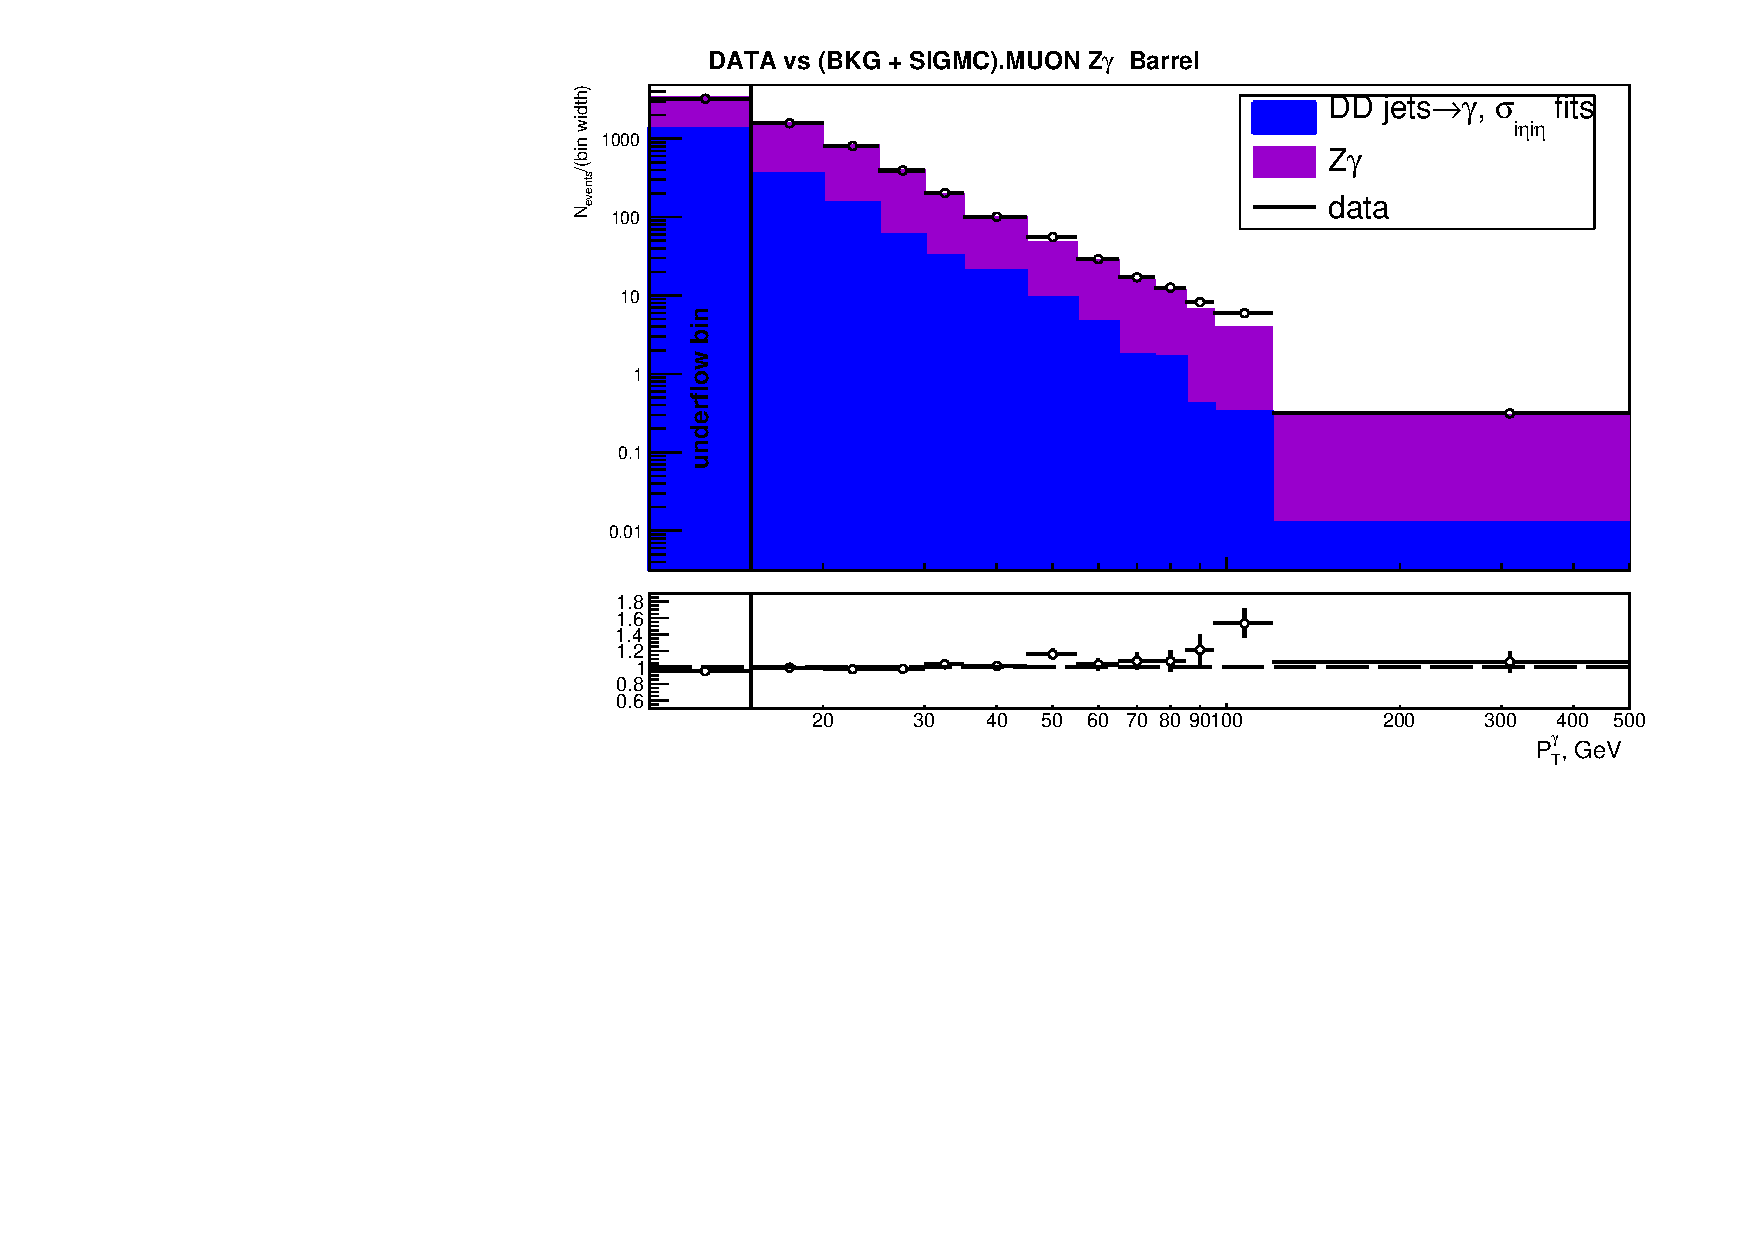
\includegraphics[width=0.45\textwidth]{../figs/figs_v11/MUON_ZGamma/PrepareYields/c_DATAvsBkgPlusSigMCc_MUON_ZGamma_TEMPL_SIHIH_UNblind__Barrel__phoEt.pdf}  \\
   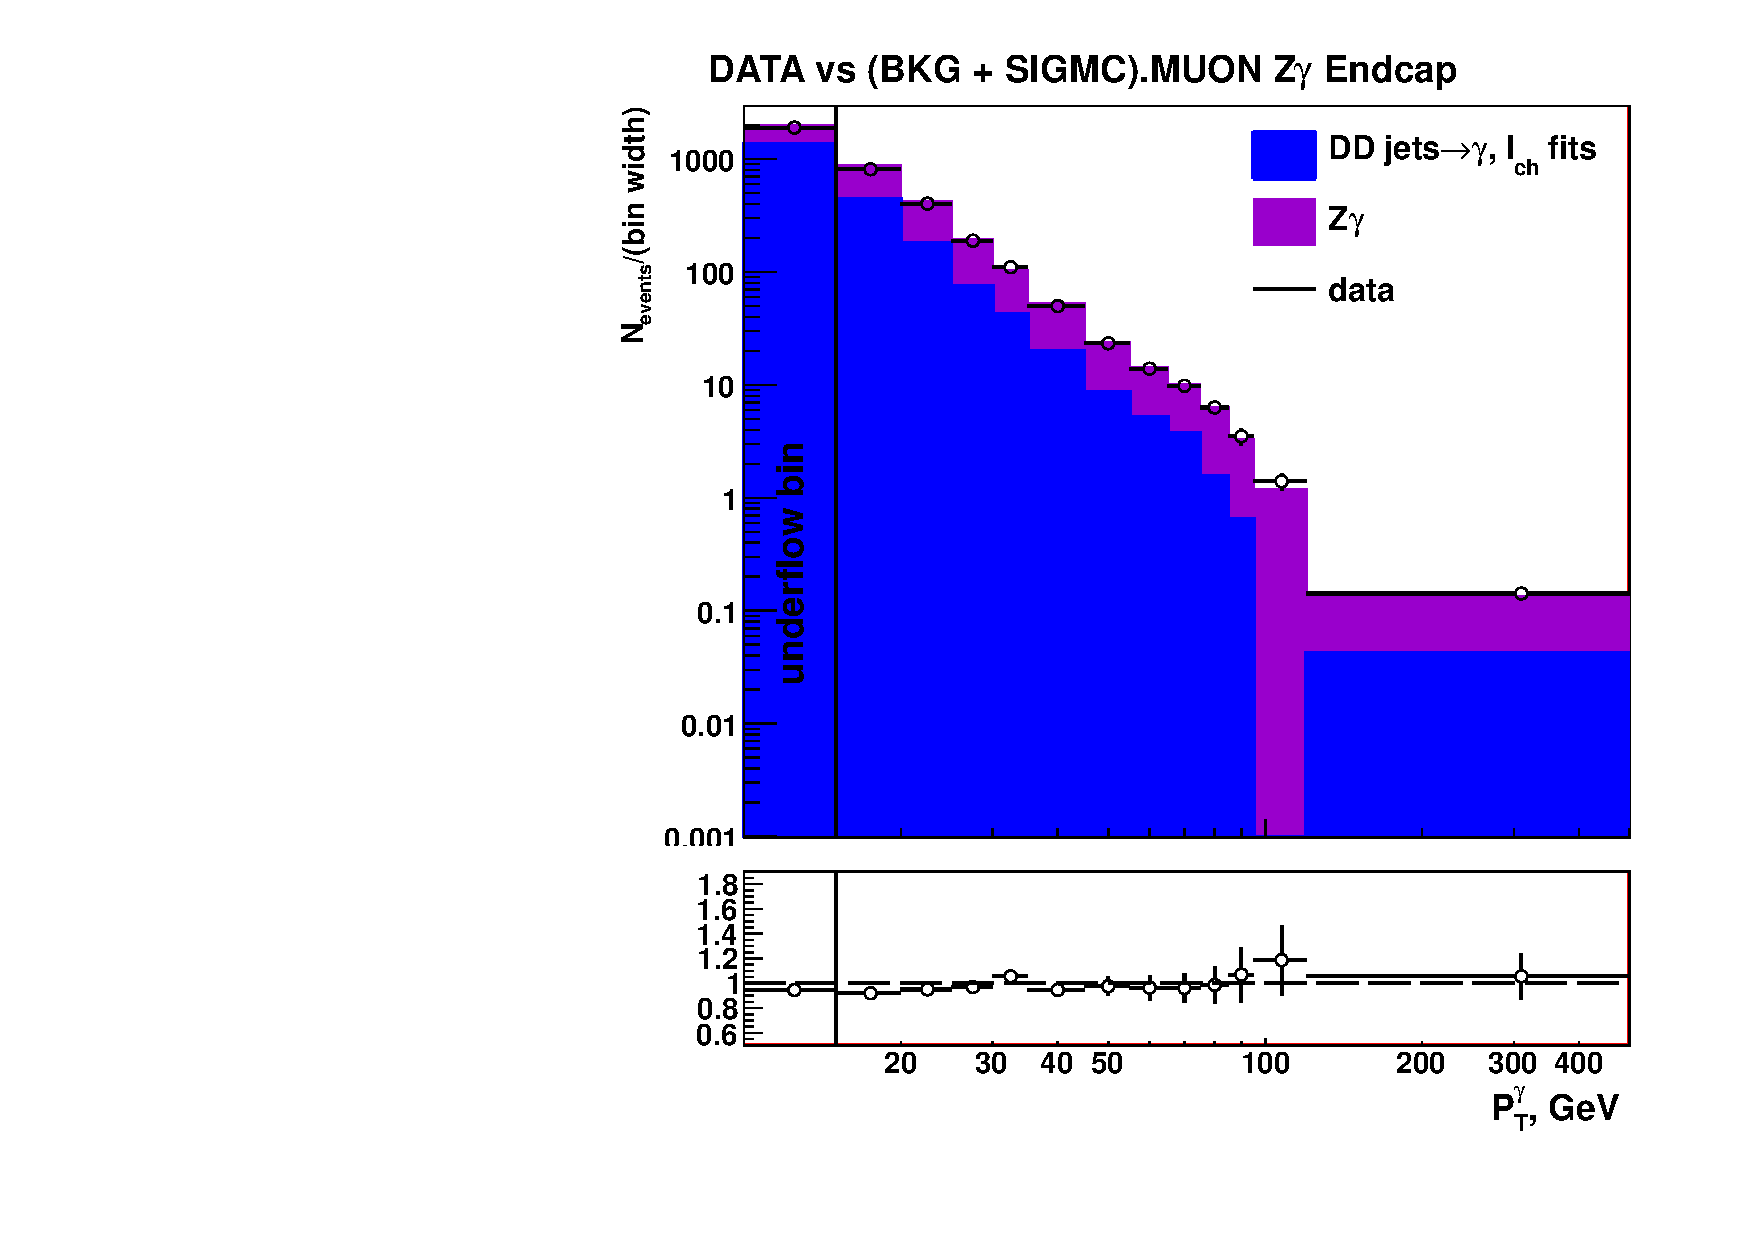
\includegraphics[width=0.45\textwidth]{../figs/figs_v11/MUON_ZGamma/PrepareYields/c_DATAvsBkgPlusSigMCc_MUON_ZGamma_TEMPL_CHISO_UNblind__Endcap__phoEt.pdf}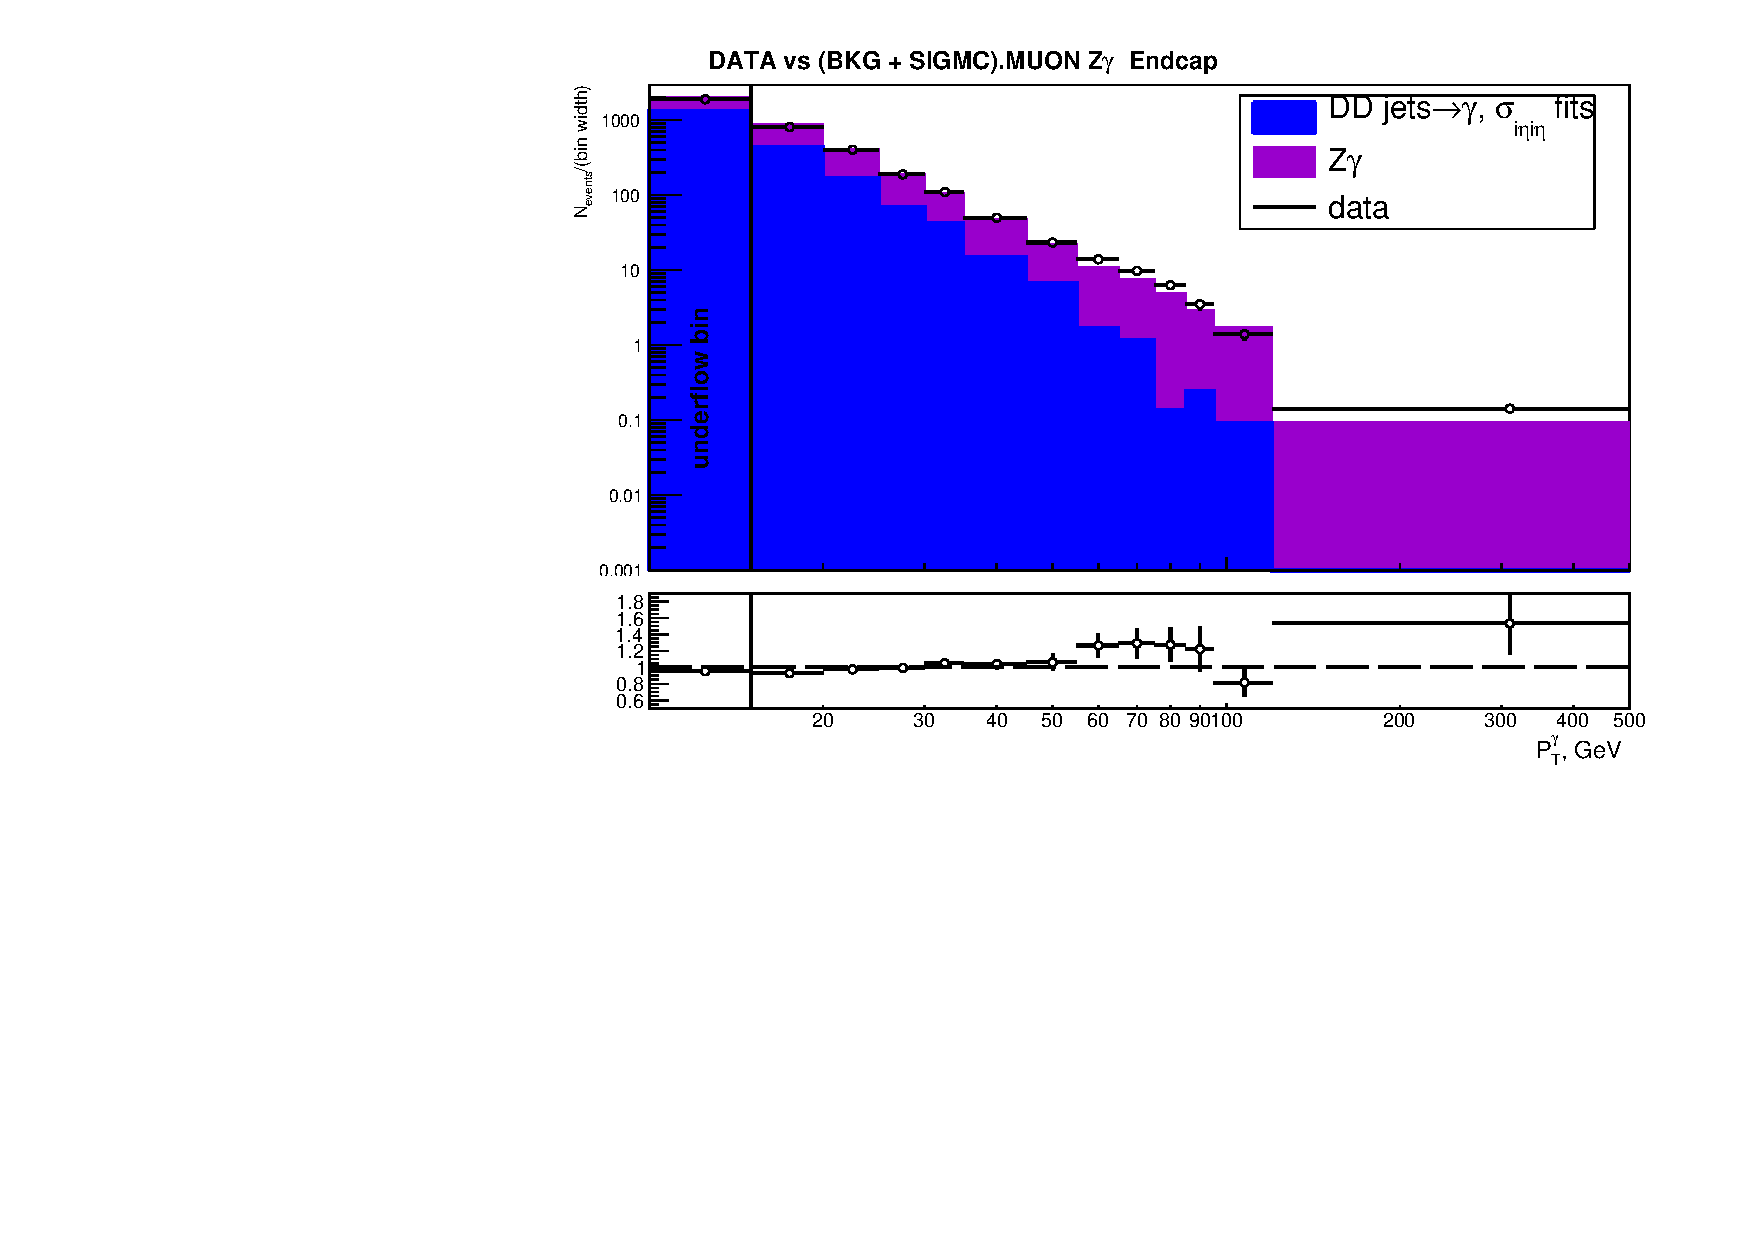
\includegraphics[width=0.45\textwidth]{../figs/figs_v11/MUON_ZGamma/PrepareYields/c_DATAvsBkgPlusSigMCc_MUON_ZGamma_TEMPL_SIHIH_UNblind__Endcap__phoEt.pdf}  \\
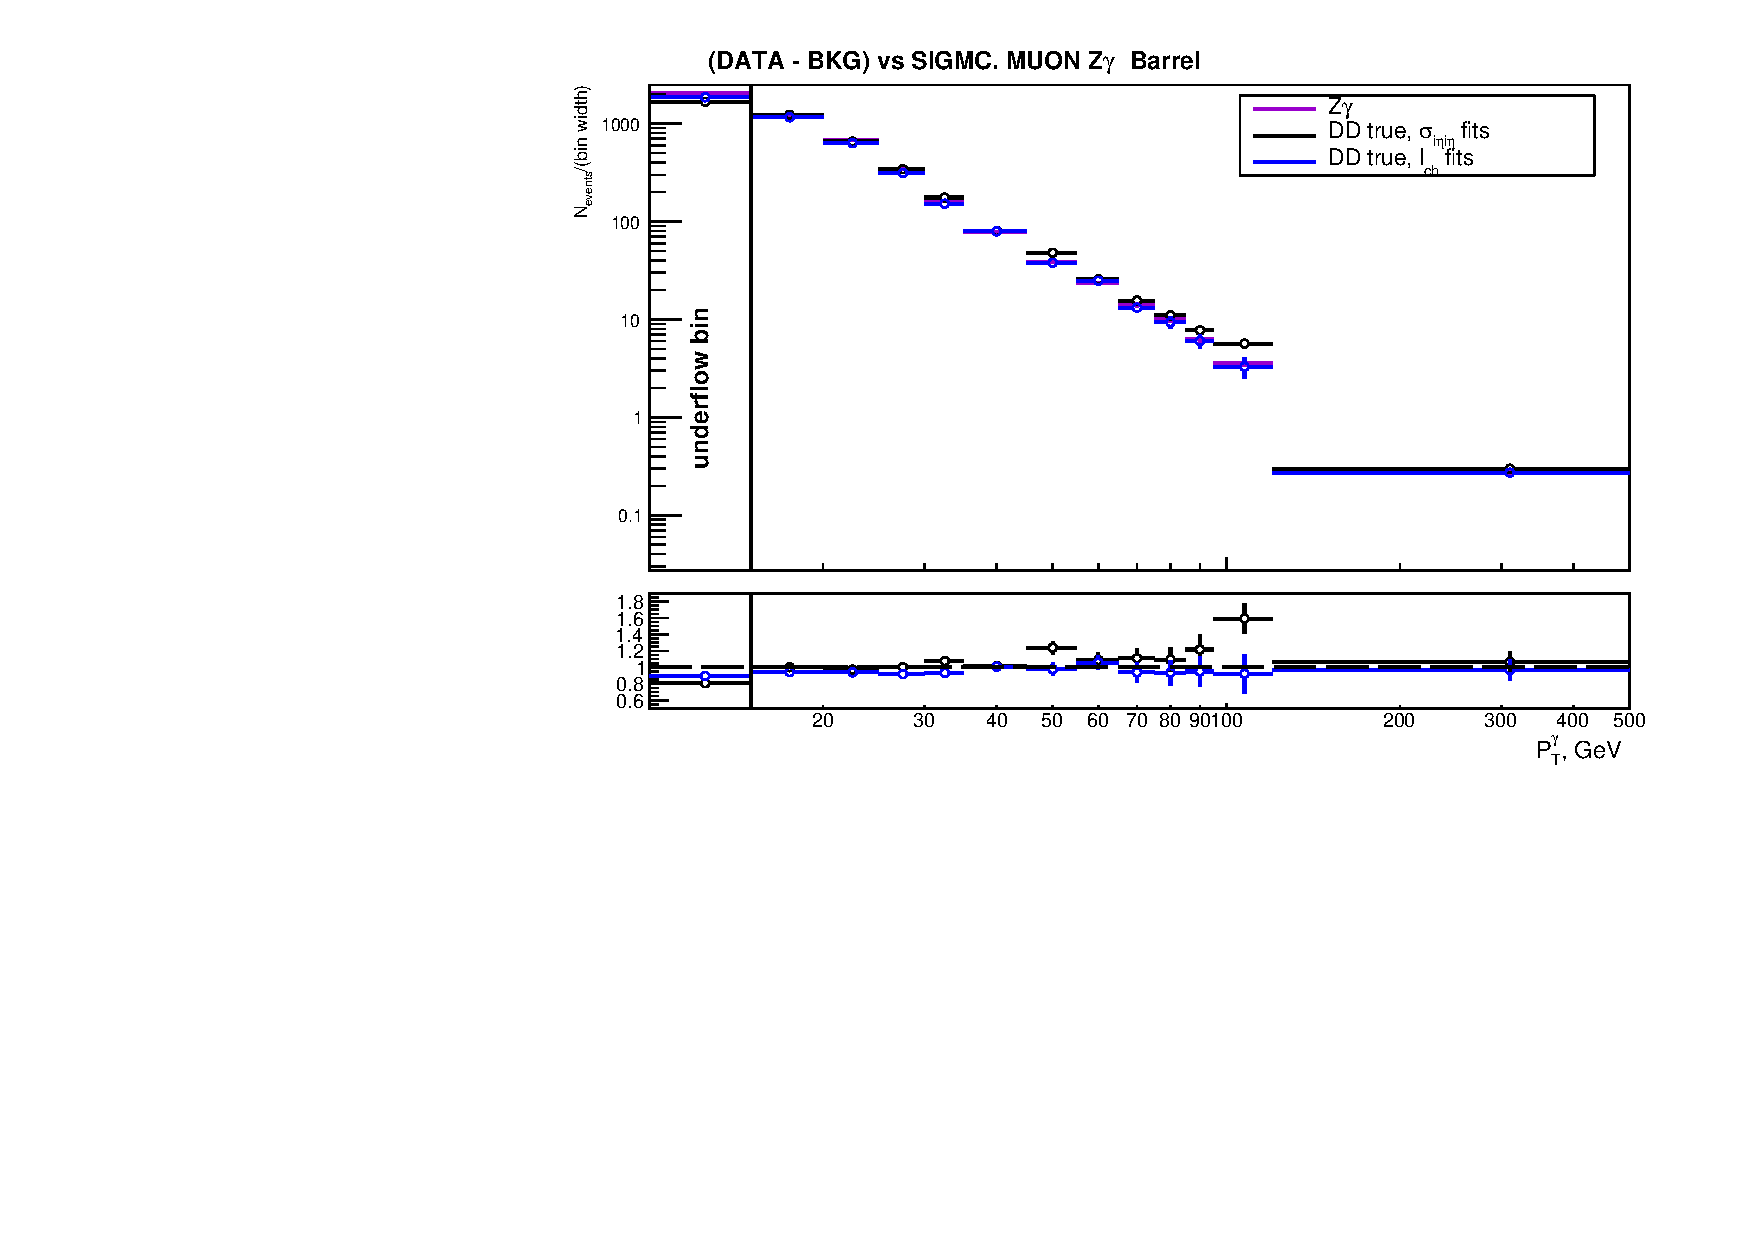
\includegraphics[width=0.45\textwidth]{../figs/figs_v11/MUON_ZGamma/PrepareYields/c_BkgSubtrDATAvsSIGMC_c_MUON_ZGamma__UNblind__Barrel__phoEt.pdf}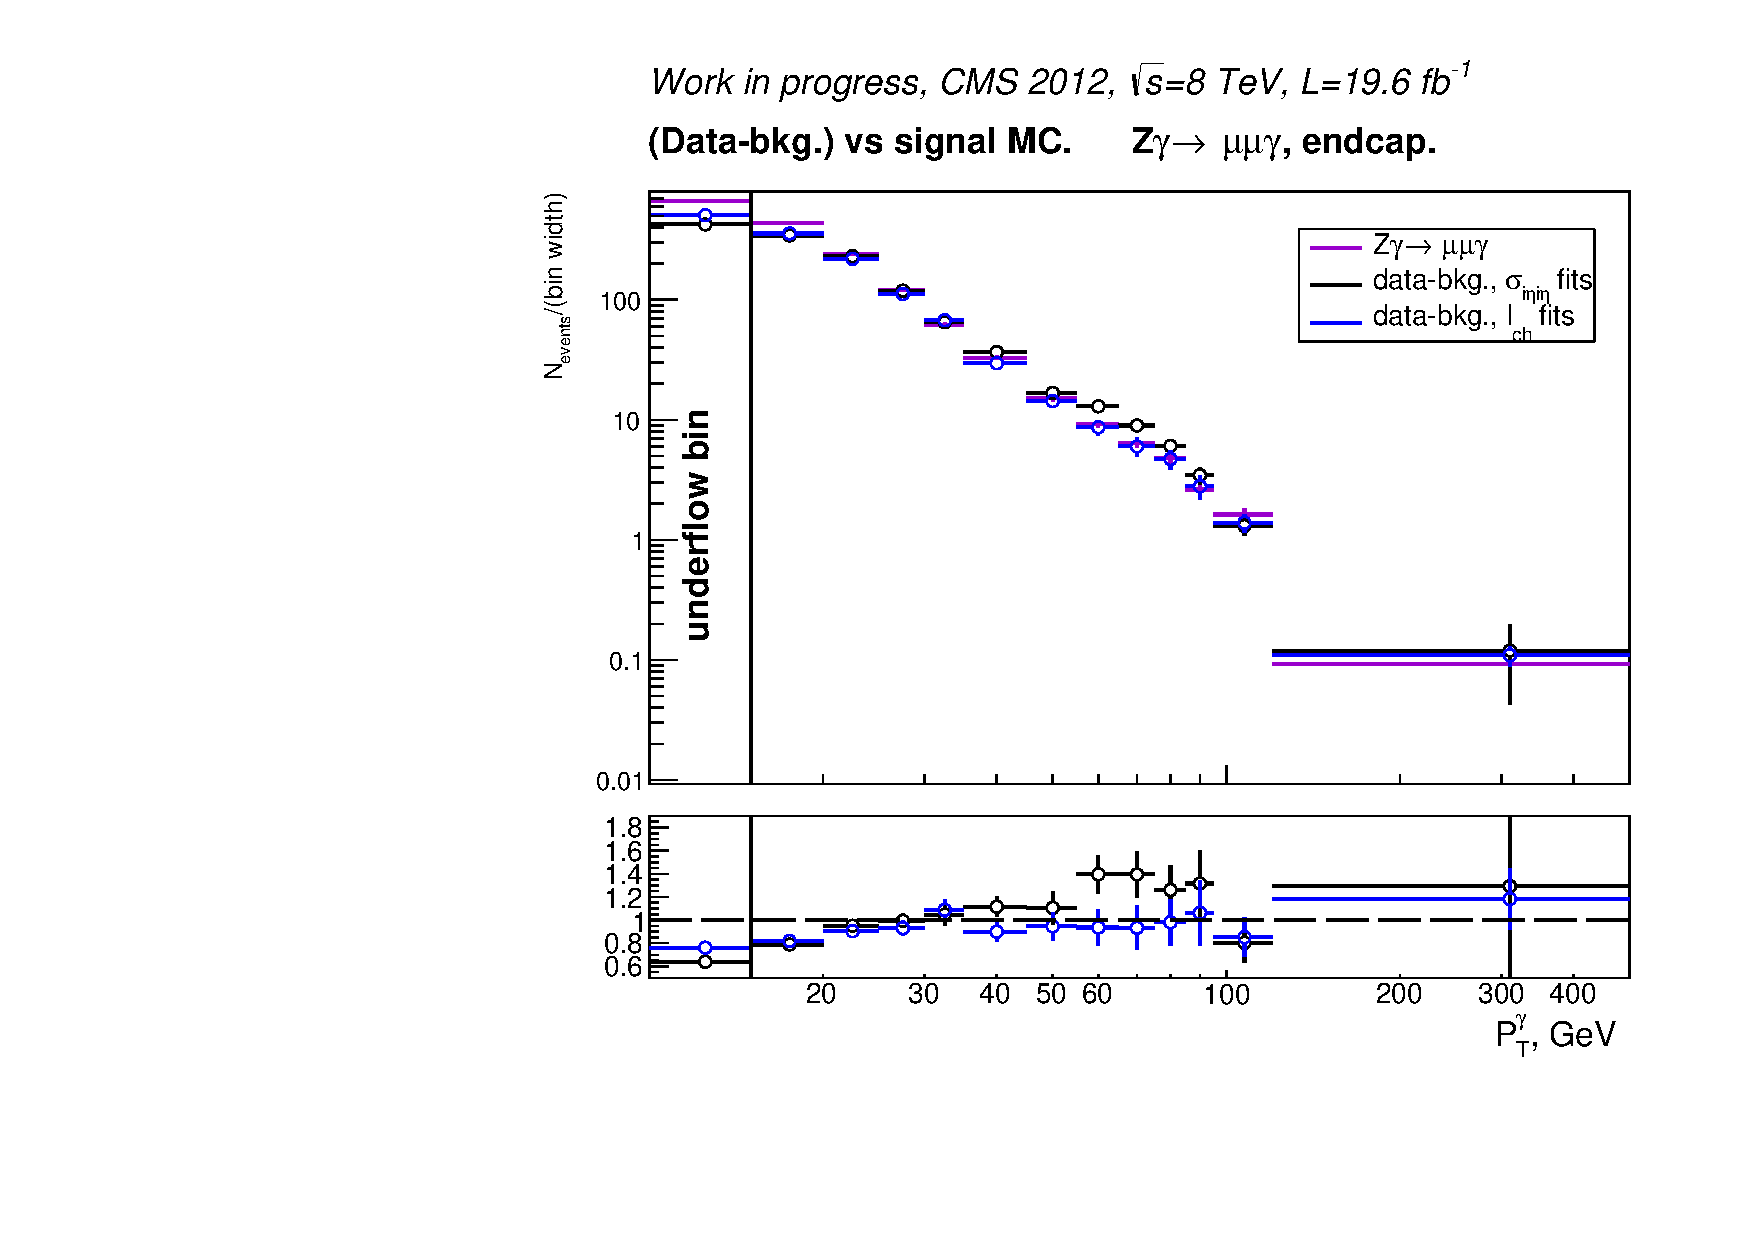
\includegraphics[width=0.45\textwidth]{../figs/figs_v11/MUON_ZGamma/PrepareYields/c_BkgSubtrDATAvsSIGMC_c_MUON_ZGamma__UNblind__Endcap__phoEt.pdf}\\
  \caption{$Z\gamma$ check. Muon channel. Top and middle: data vs fake-$\gamma$ background derived from the template method + real-$\gamma$ background predicted by dedicated MC samples + signal MC, with $I_{ch}$ and $\sigma_{i\etai\eta}$ used as fit variables. Bottom: data yields after full background subtraction vs signal MC. $I_{ch}$ vs $\sigma_{i\etai\eta}$ fit results. }
  \label{fig:DDvsMC_Zg_Data_MUON}
  \end{center}
\end{figure}


\begin{figure}[htb]
  \begin{center}
   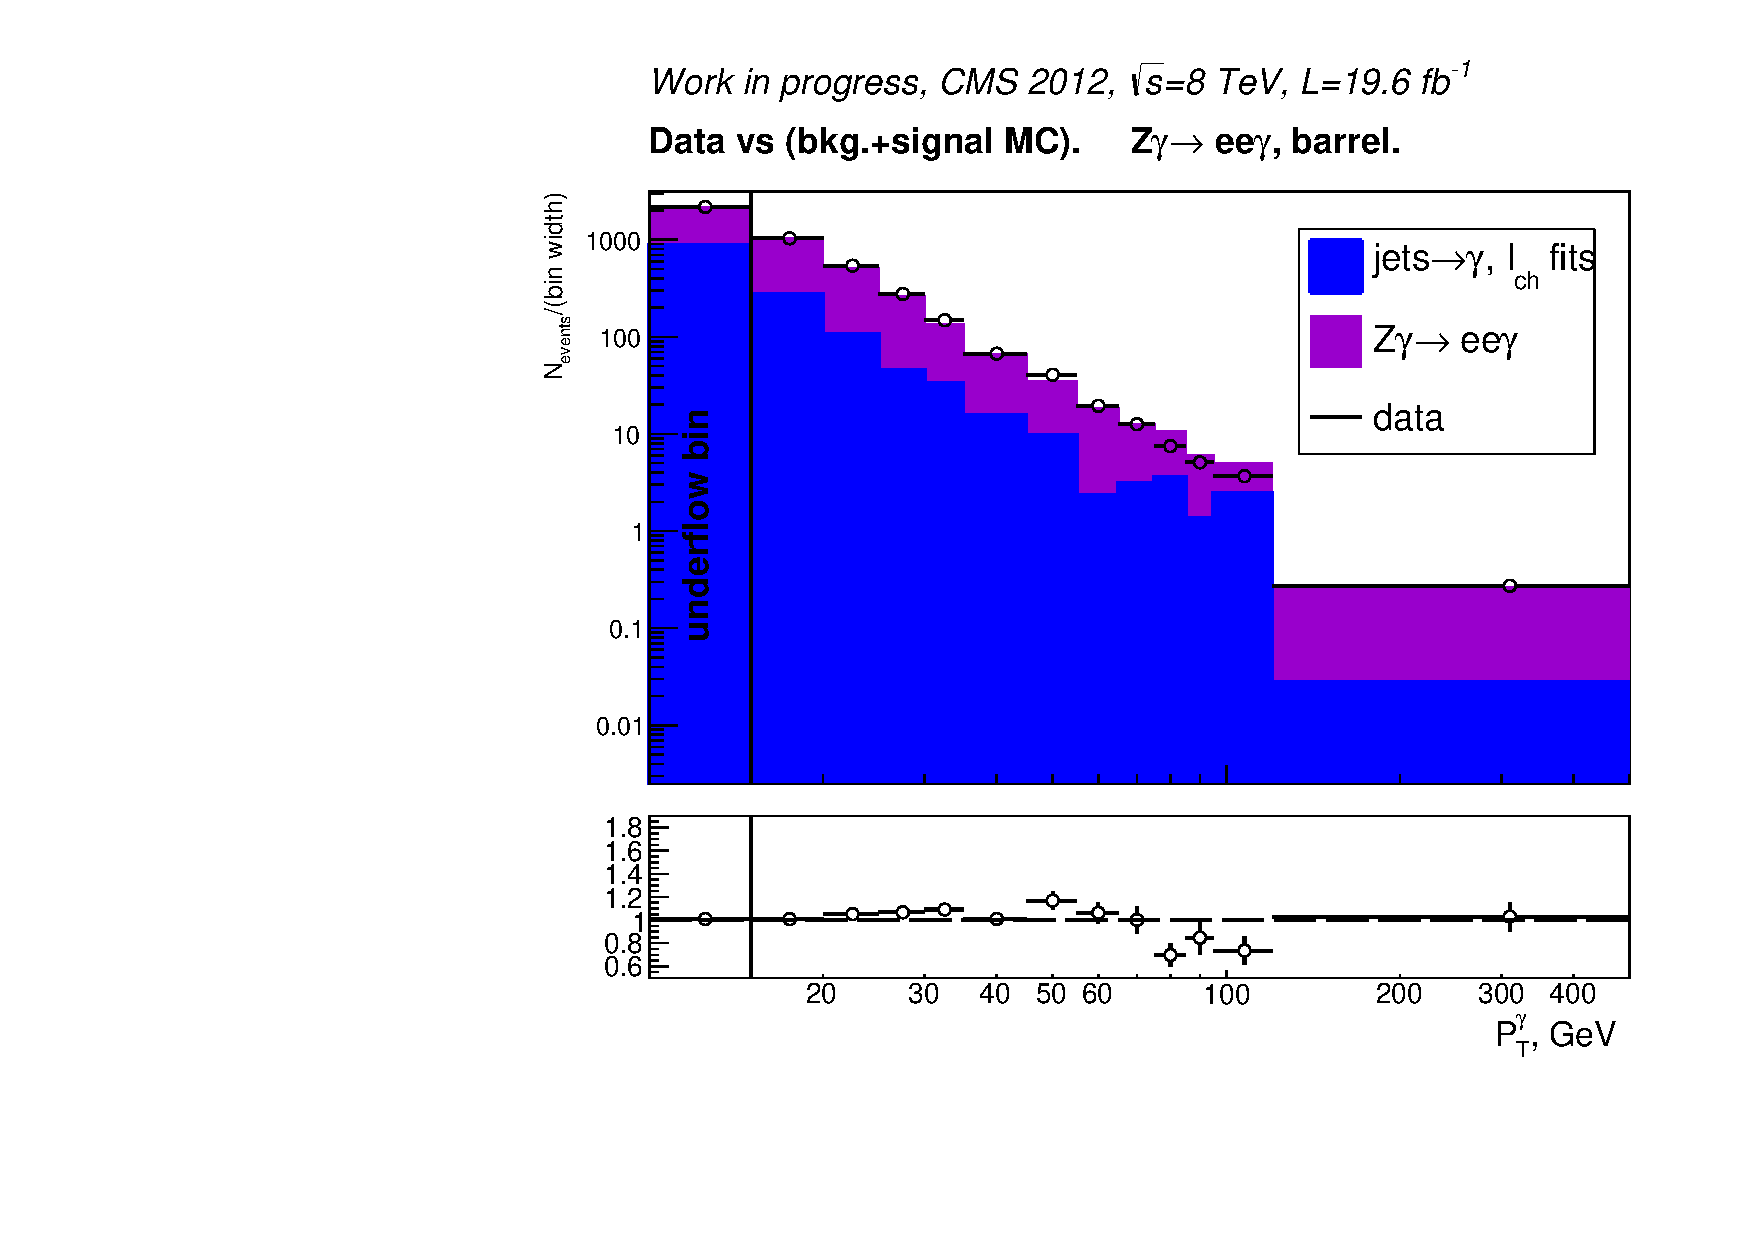
\includegraphics[width=0.45\textwidth]{../figs/figs_v11/ELECTRON_ZGamma/PrepareYields/c_DATAvsBkgPlusSigMCc_ELECTRON_ZGamma_TEMPL_CHISO_UNblind__Barrel__phoEt.pdf}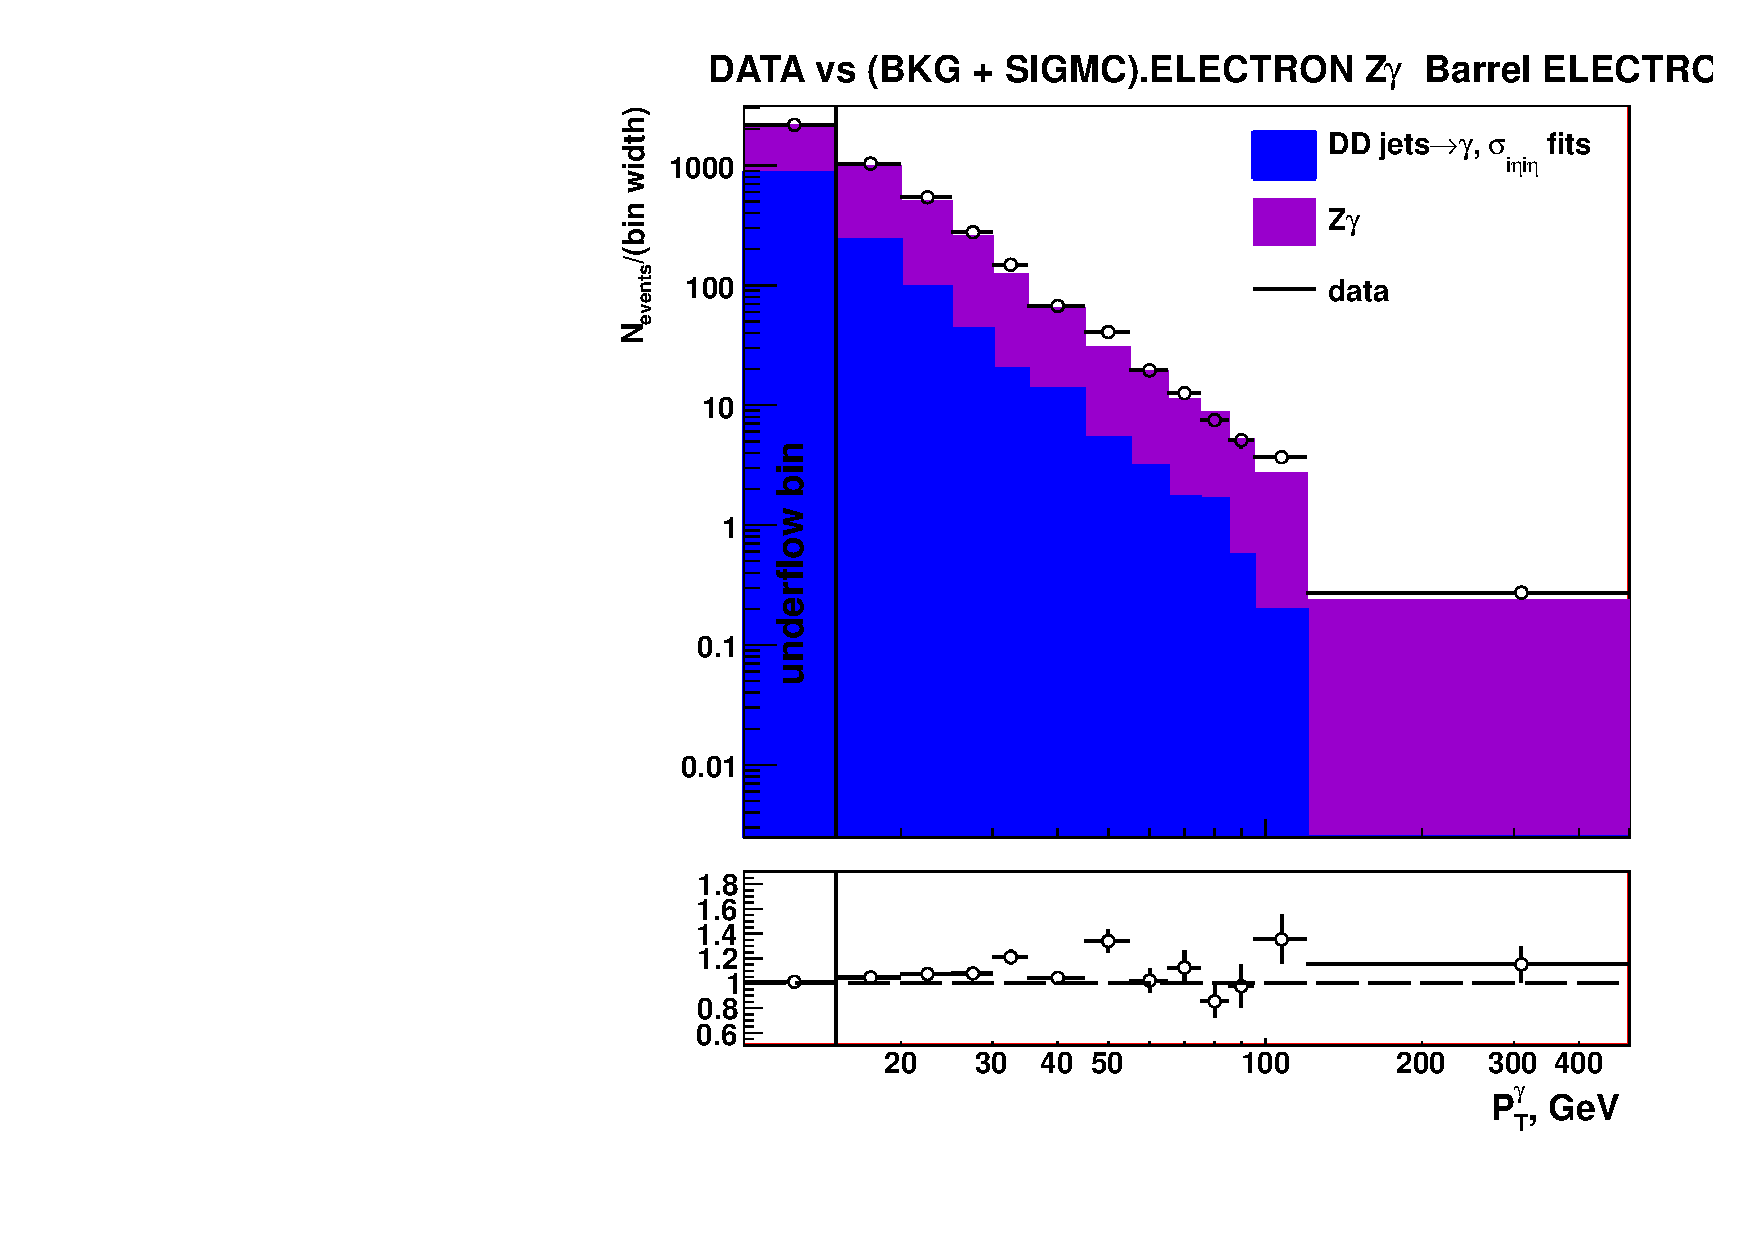
\includegraphics[width=0.45\textwidth]{../figs/figs_v11/ELECTRON_ZGamma/PrepareYields/c_DATAvsBkgPlusSigMCc_ELECTRON_ZGamma_TEMPL_SIHIH_UNblind__Barrel__phoEt.pdf}  \\
   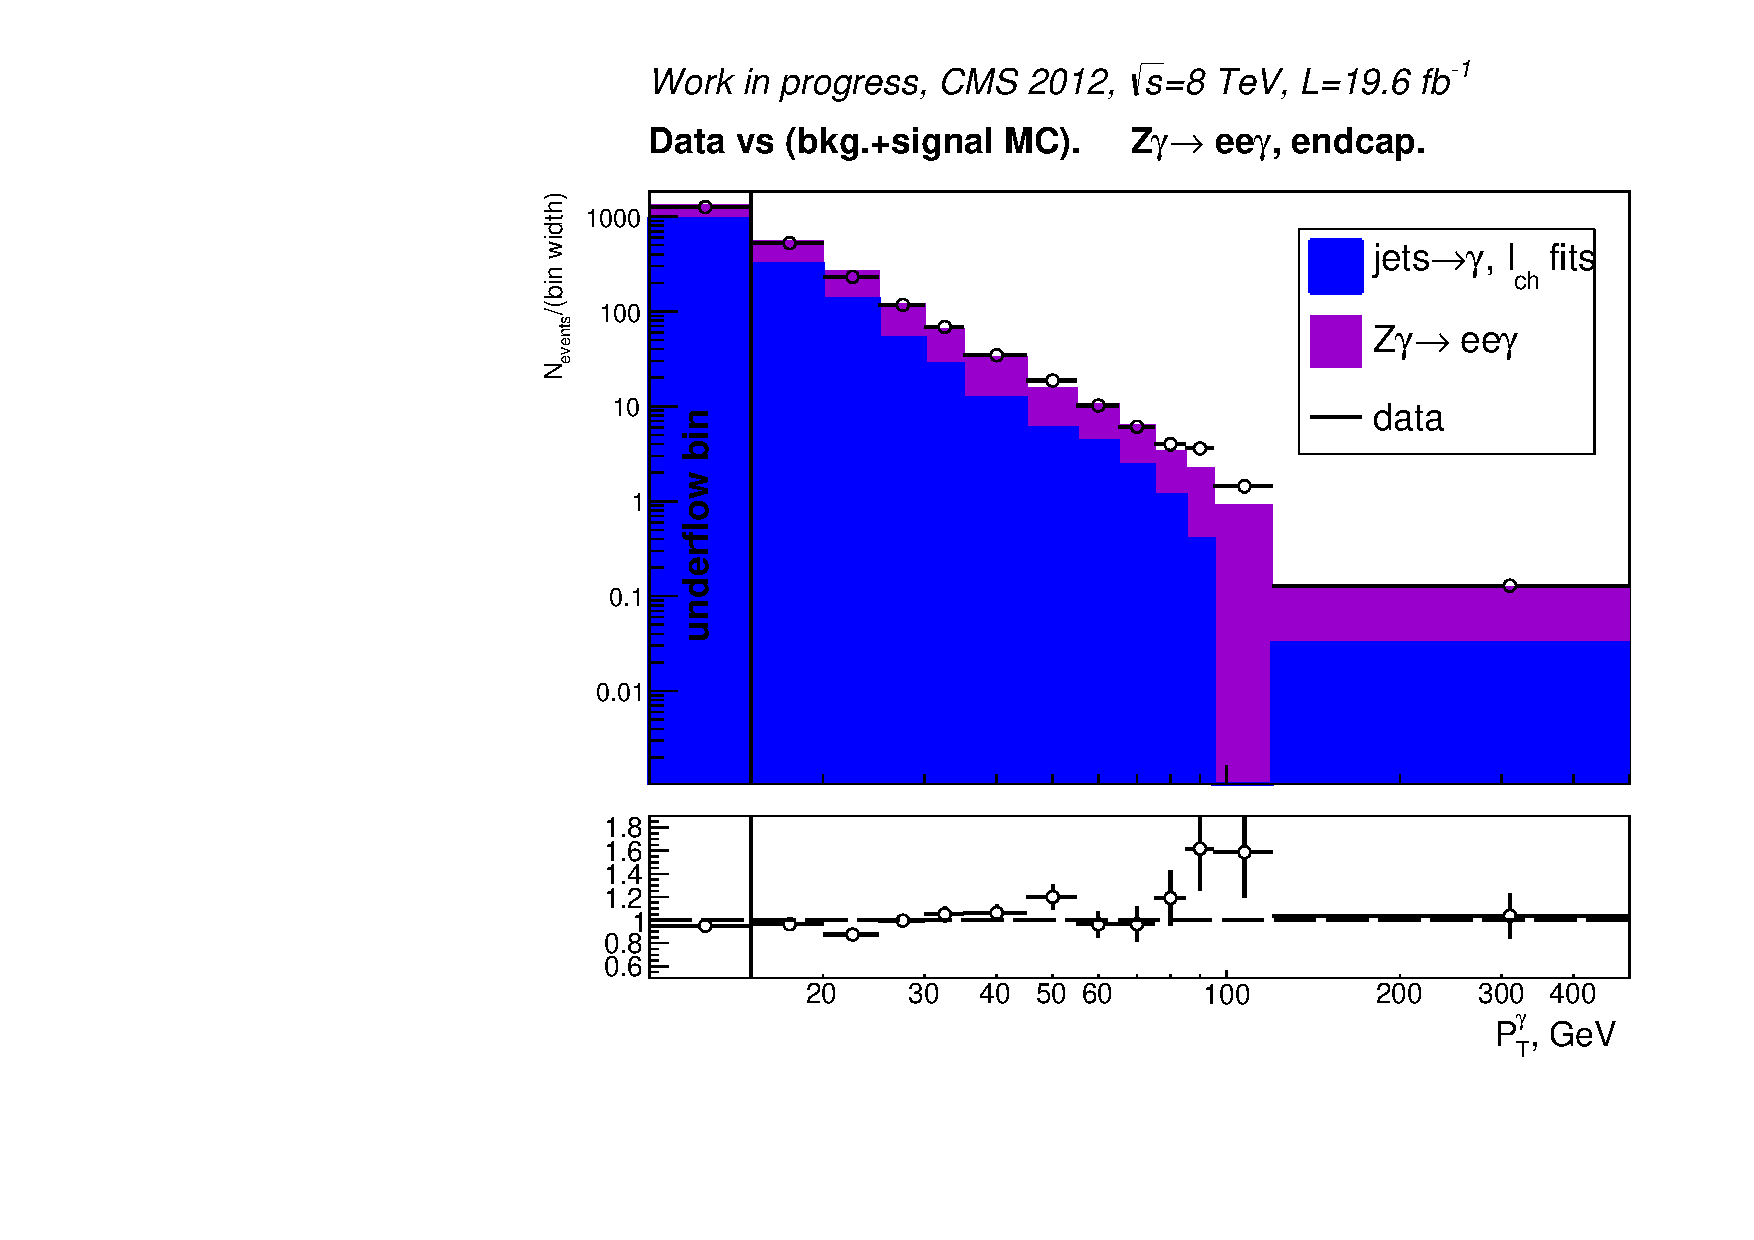
\includegraphics[width=0.45\textwidth]{../figs/figs_v11/ELECTRON_ZGamma/PrepareYields/c_DATAvsBkgPlusSigMCc_ELECTRON_ZGamma_TEMPL_CHISO_UNblind__Endcap__phoEt.pdf}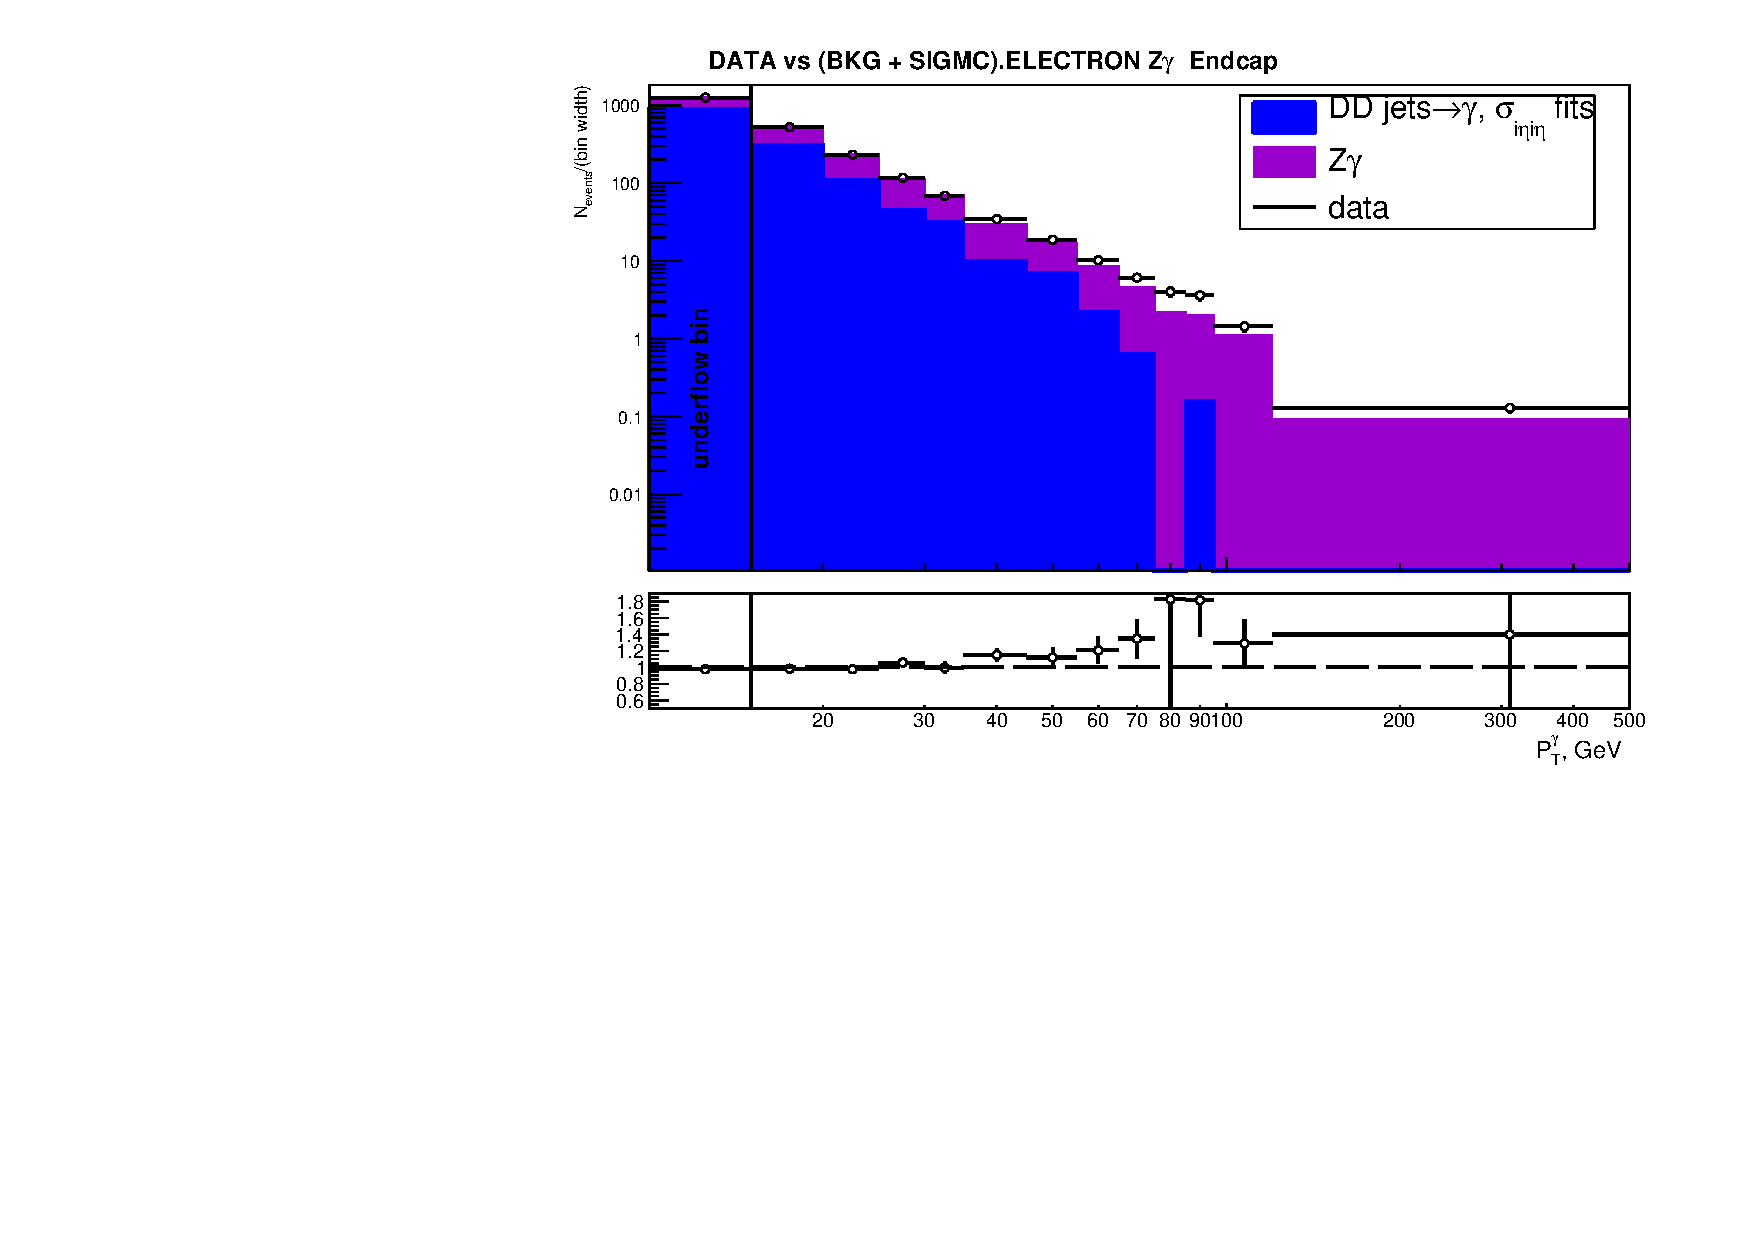
\includegraphics[width=0.45\textwidth]{../figs/figs_v11/ELECTRON_ZGamma/PrepareYields/c_DATAvsBkgPlusSigMCc_ELECTRON_ZGamma_TEMPL_SIHIH_UNblind__Endcap__phoEt.pdf}  \\
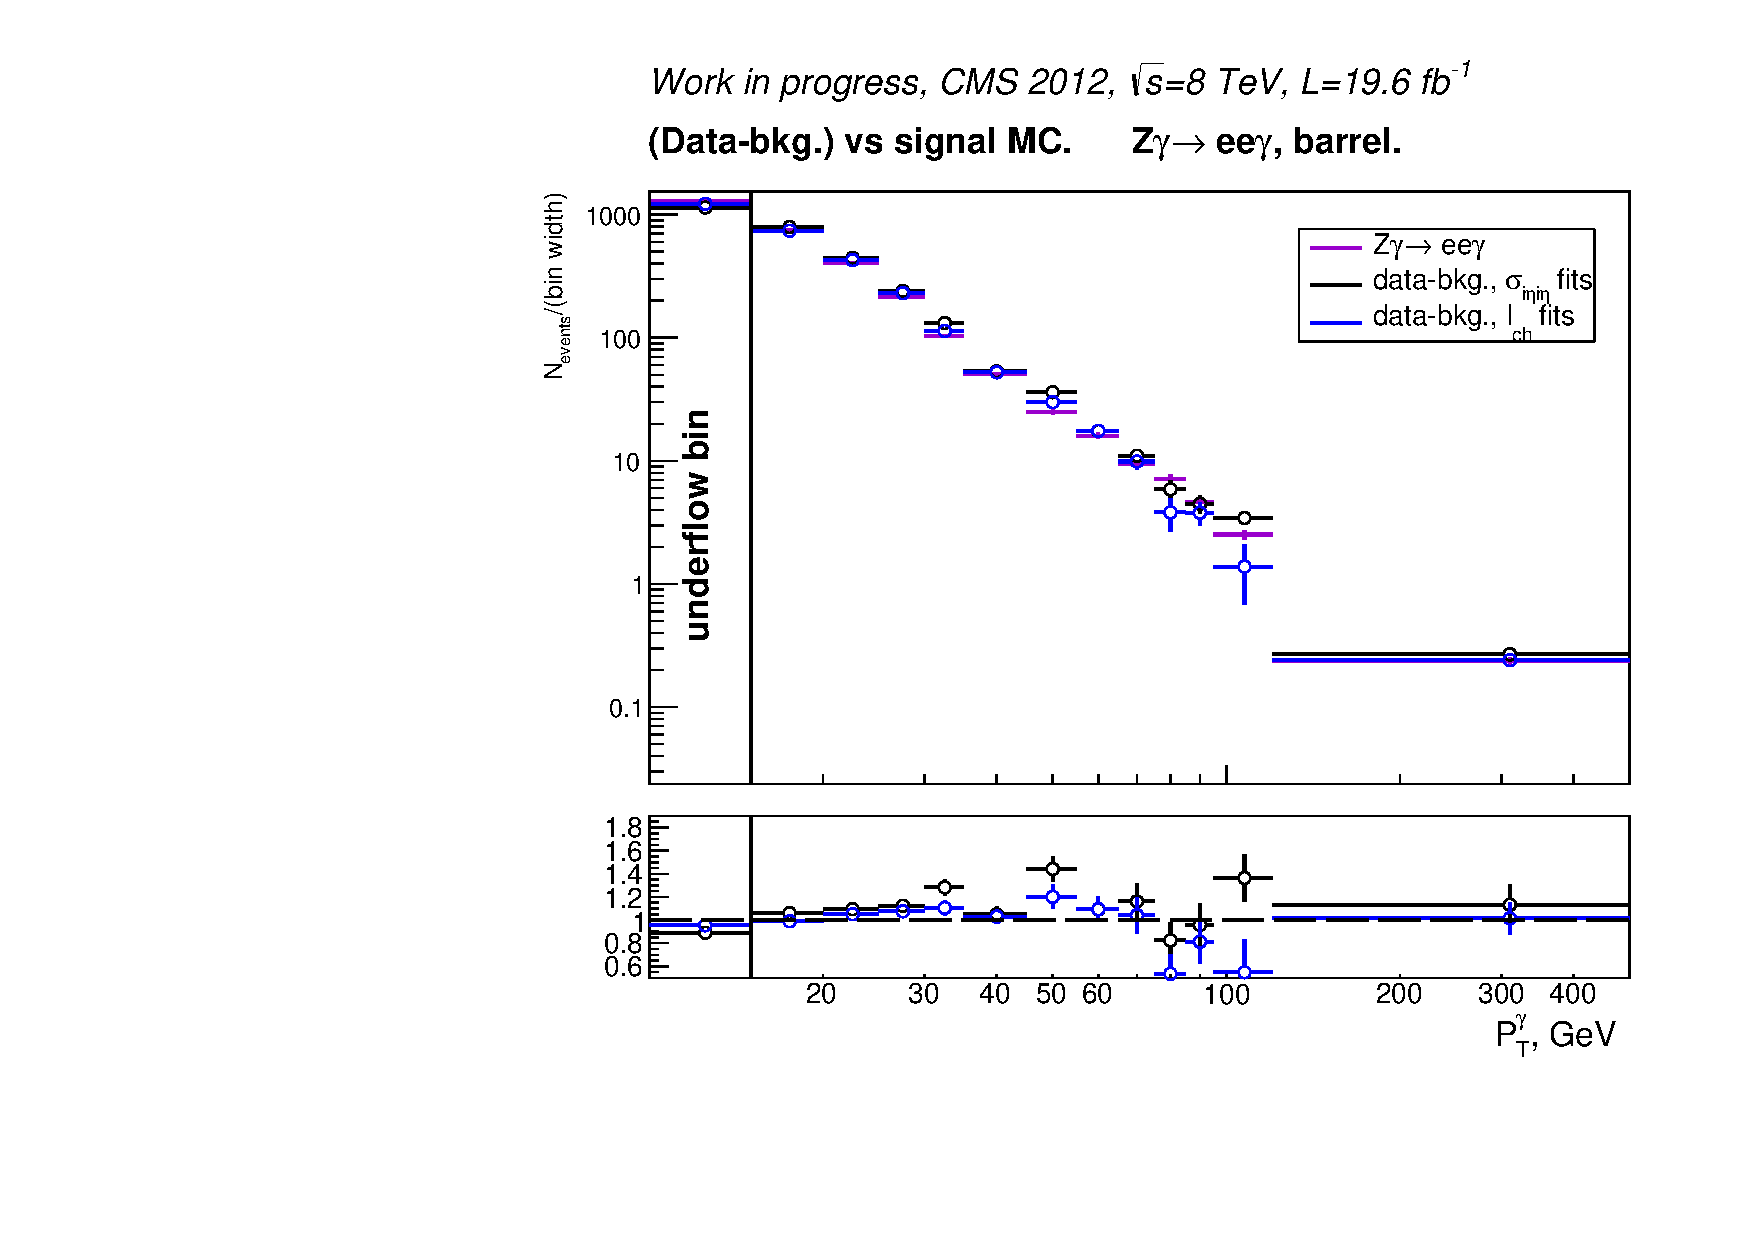
\includegraphics[width=0.45\textwidth]{../figs/figs_v11/ELECTRON_ZGamma/PrepareYields/c_BkgSubtrDATAvsSIGMC_c_ELECTRON_ZGamma__UNblind__Barrel__phoEt.pdf}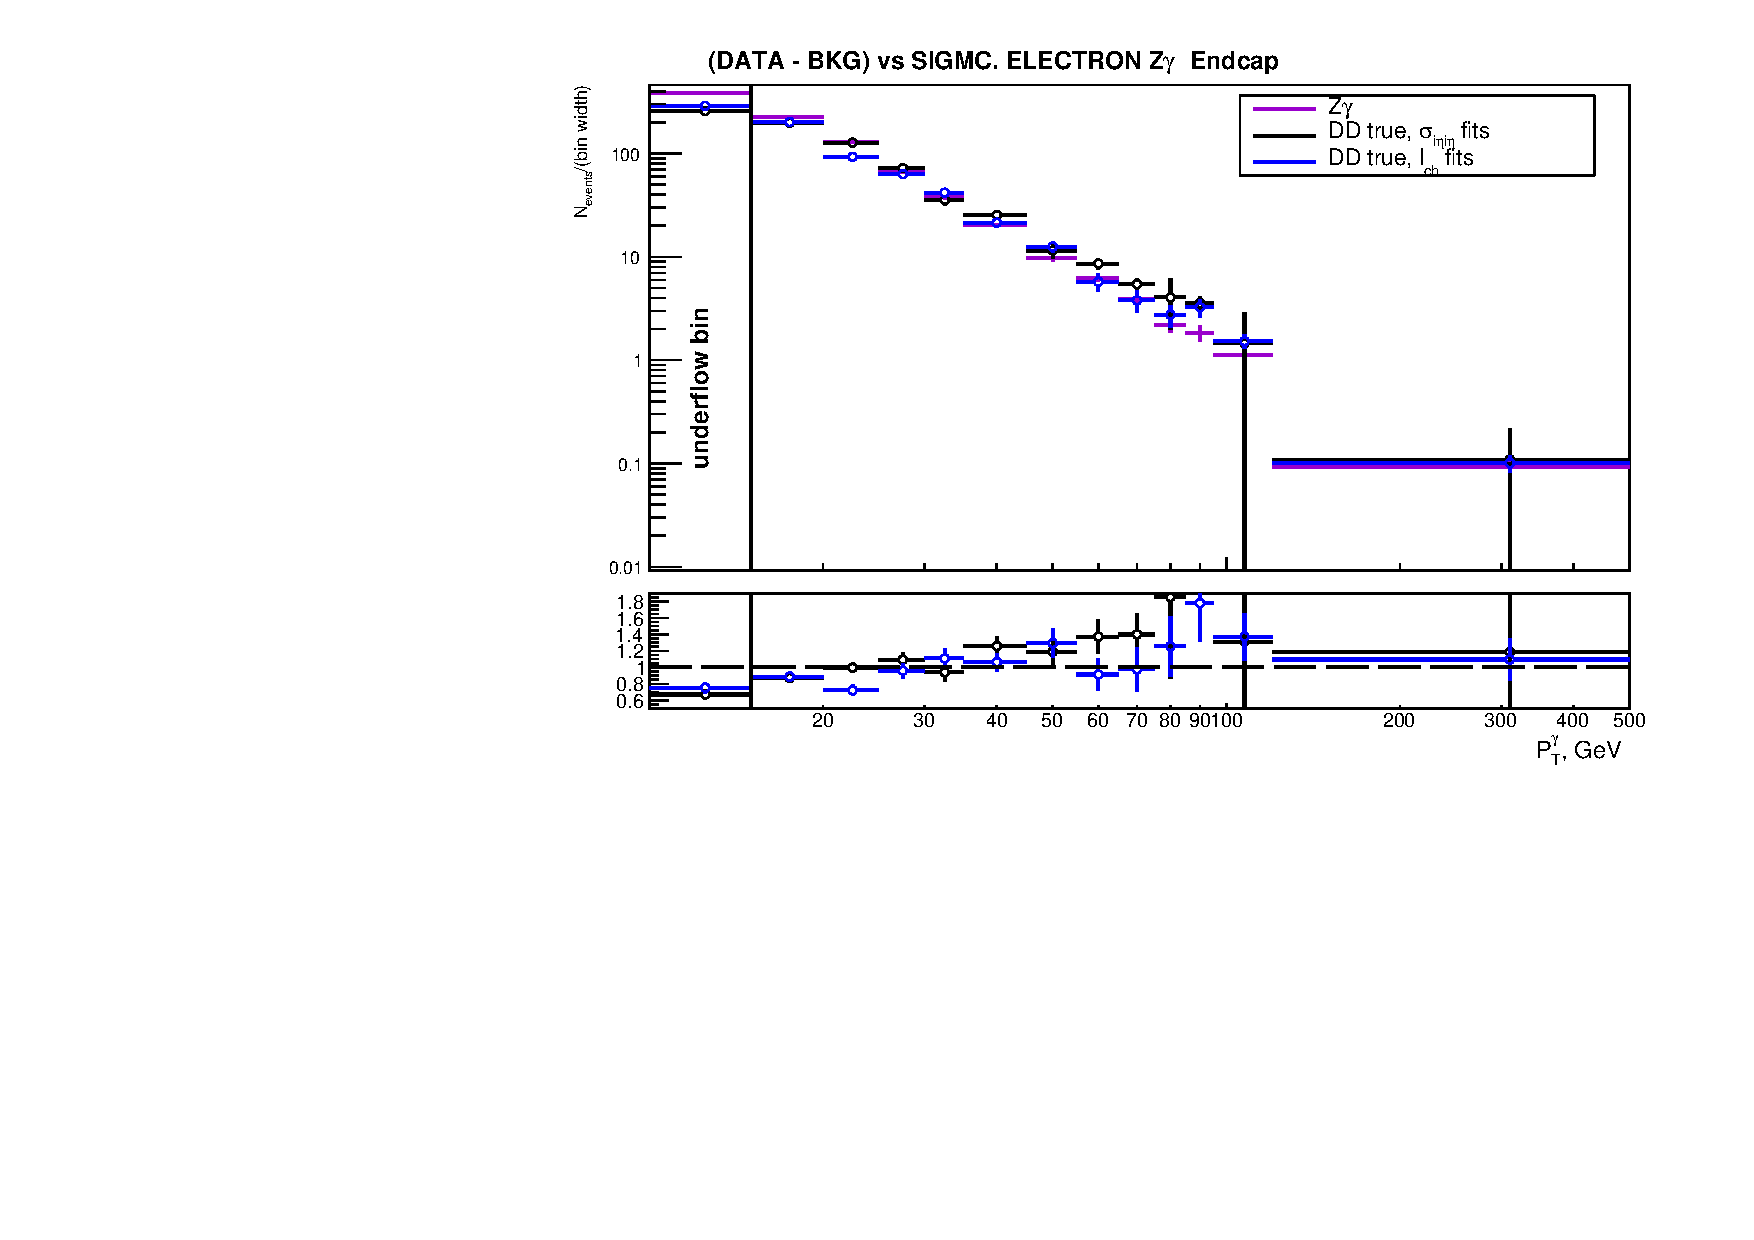
\includegraphics[width=0.45\textwidth]{../figs/figs_v11/ELECTRON_ZGamma/PrepareYields/c_BkgSubtrDATAvsSIGMC_c_ELECTRON_ZGamma__UNblind__Endcap__phoEt.pdf}\\
  \caption{$Z\gamma$ check. Electron channel. Top and middle: data vs fake-$\gamma$ background derived from the template method + real-$\gamma$ background predicted by dedicated MC samples + signal MC, with $I_{ch}$ and $\sigma_{i\etai\eta}$ used as fit variables. Bottom: data yields after full background subtraction vs signal MC. $I_{ch}$ vs $\sigma_{i\etai\eta}$ fit results. }
  \label{fig:DDvsMC_Zg_Data_ELECTRON}
  \end{center}
\end{figure}

\begin{figure}[htb]
  \begin{center}
   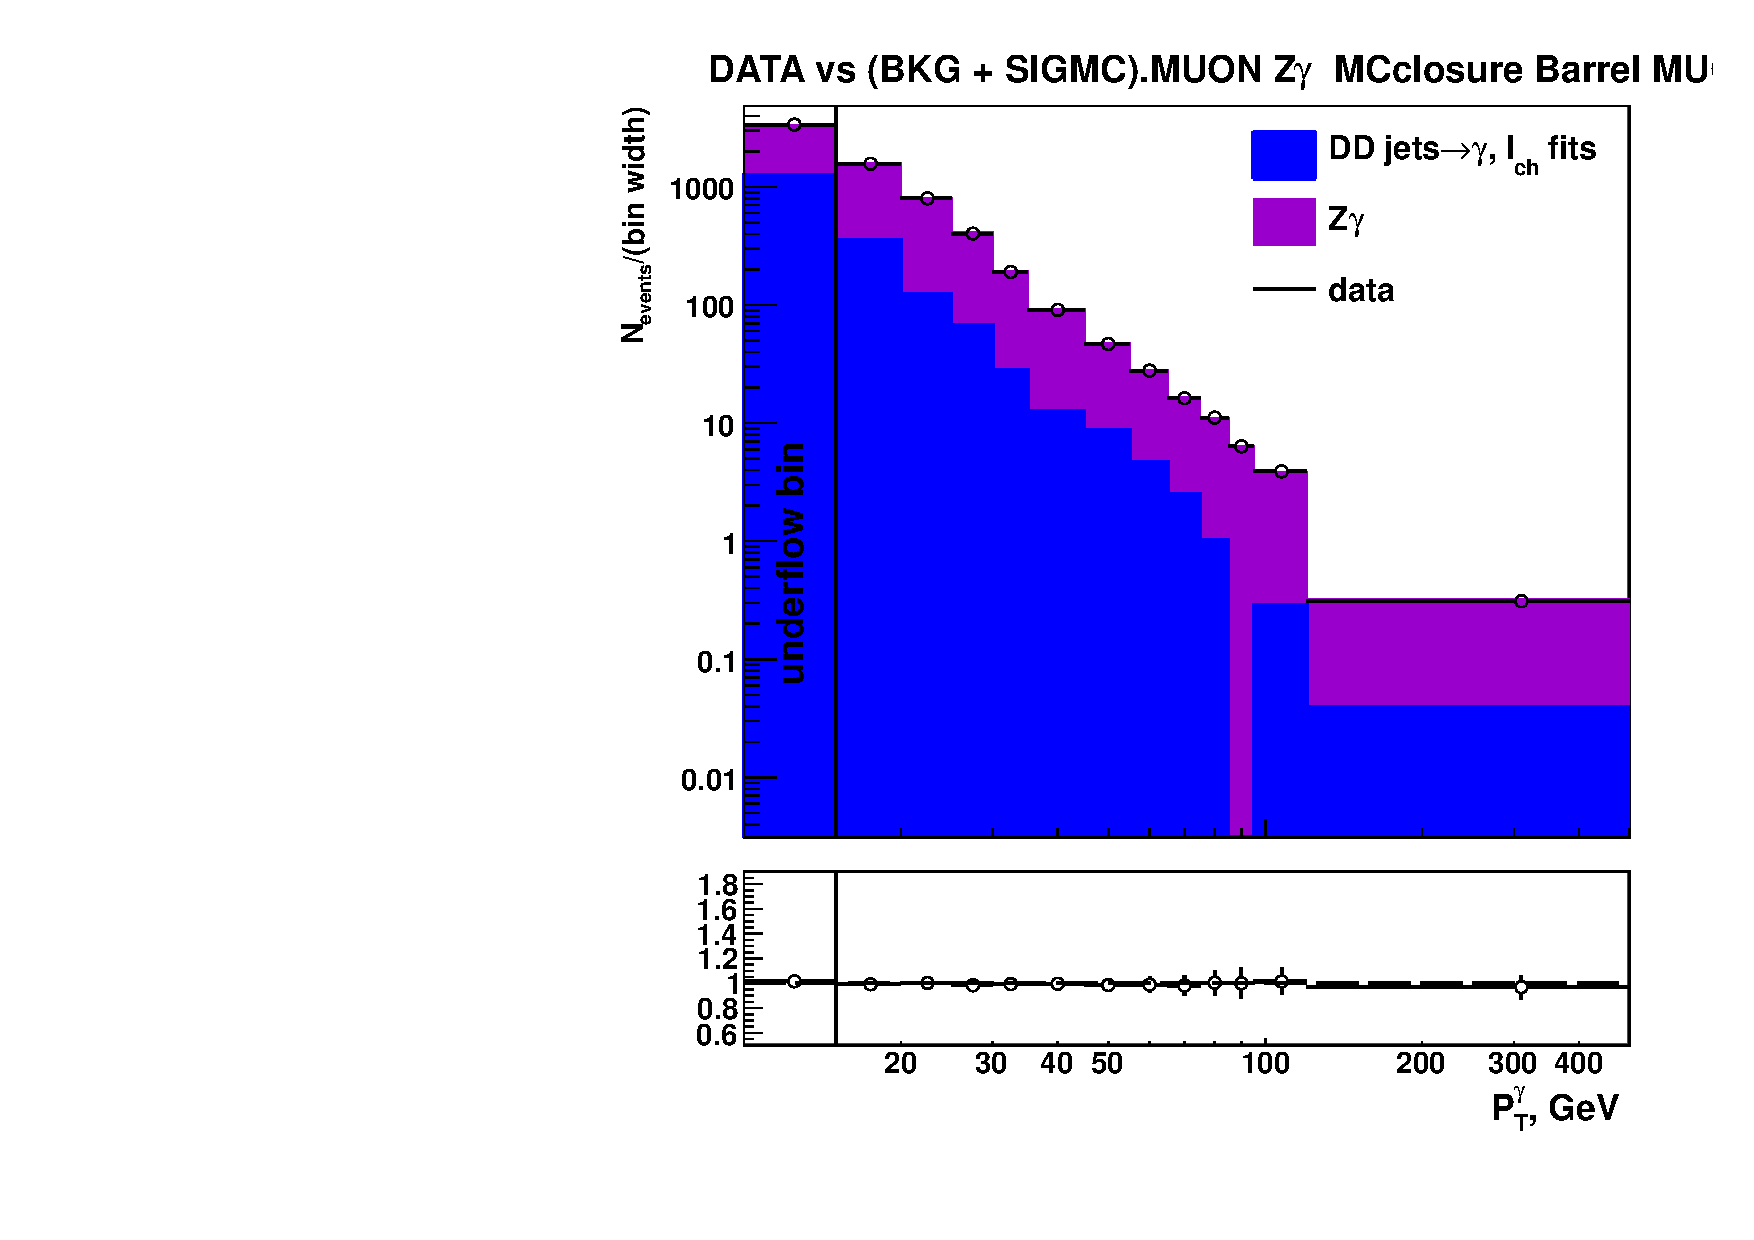
\includegraphics[width=0.45\textwidth]{../figs/figs_v11/MUON_ZGamma/PrepareYields/c_DATAvsBkgPlusSigMCc_MUON_ZGamma_TEMPL_CHISO_UNblind_MCclosure__Barrel__phoEt_MCclosure.pdf}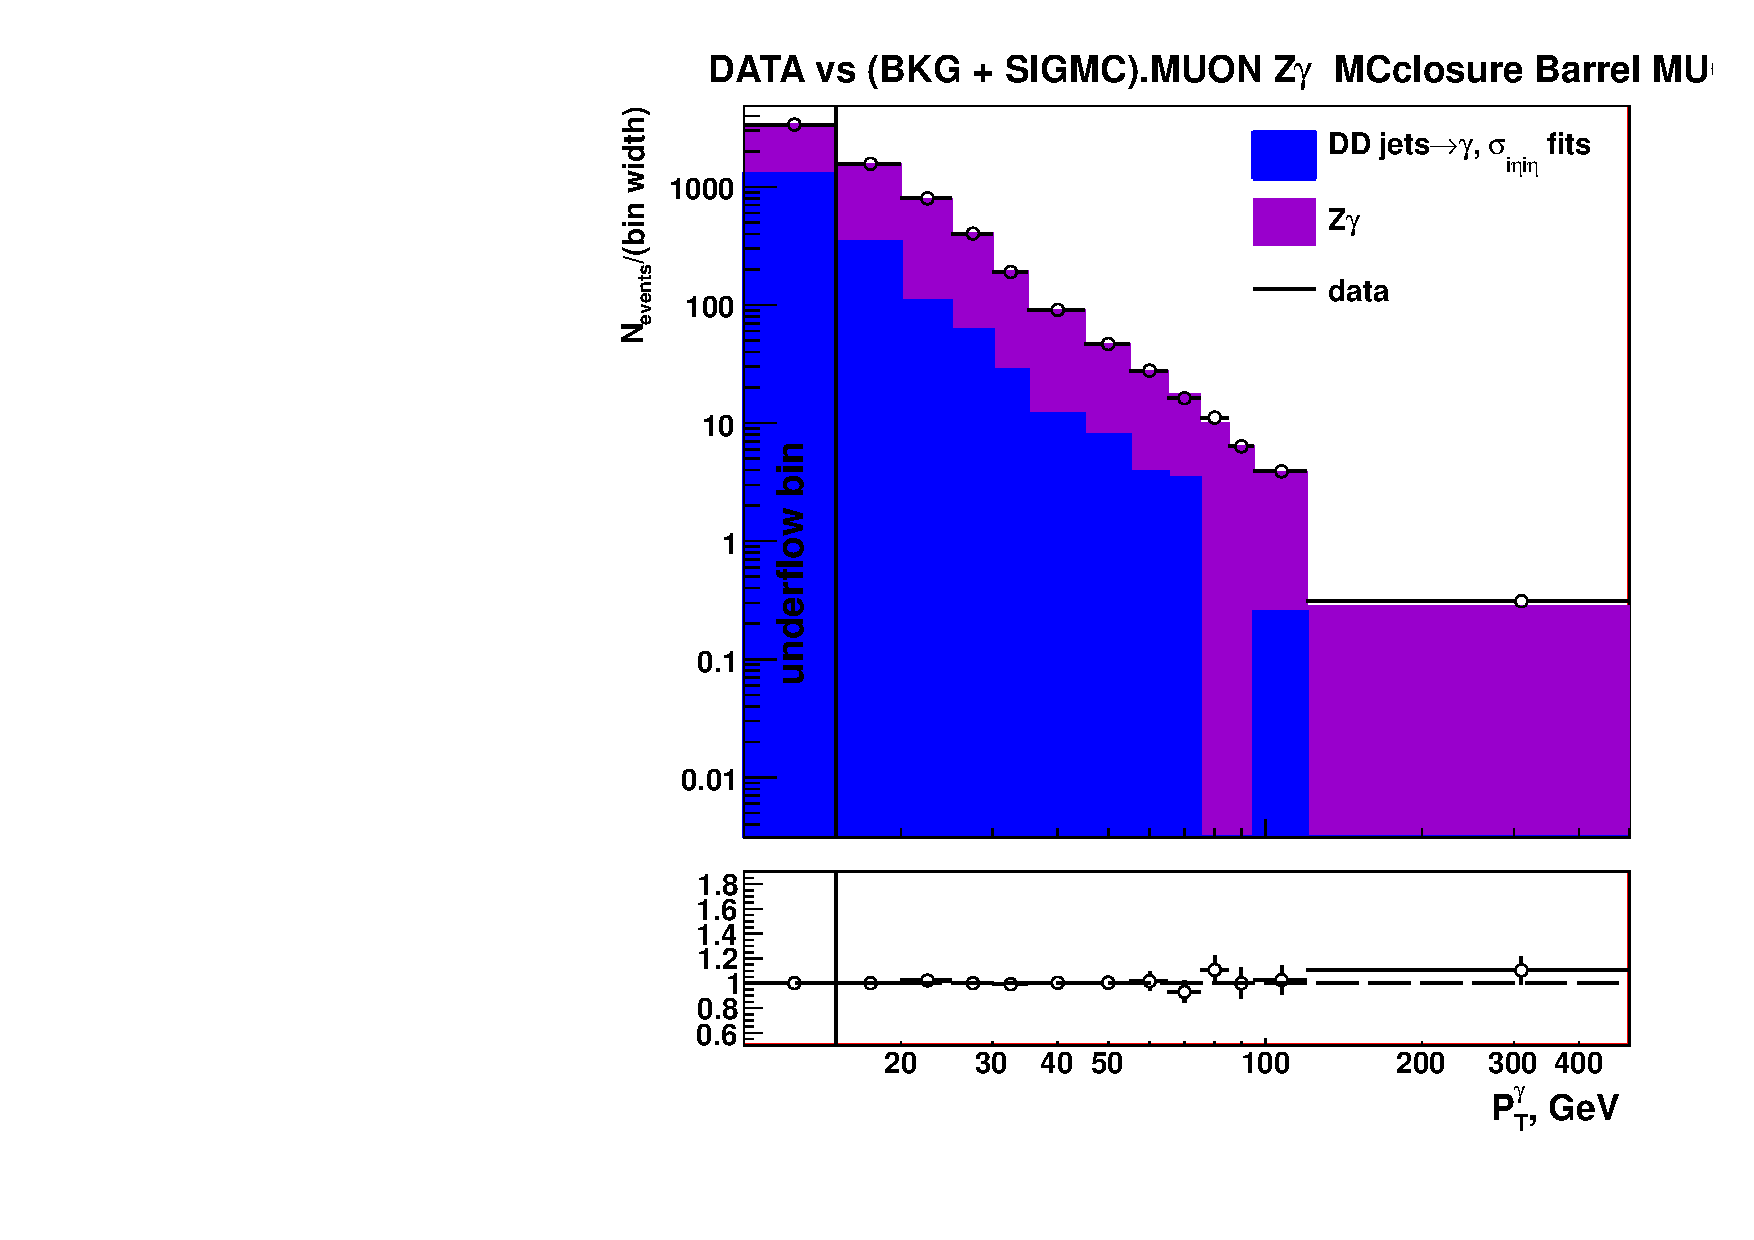
\includegraphics[width=0.45\textwidth]{../figs/figs_v11/MUON_ZGamma/PrepareYields/c_DATAvsBkgPlusSigMCc_MUON_ZGamma_TEMPL_SIHIH_UNblind_MCclosure__Barrel__phoEt_MCclosure.pdf}  \\
   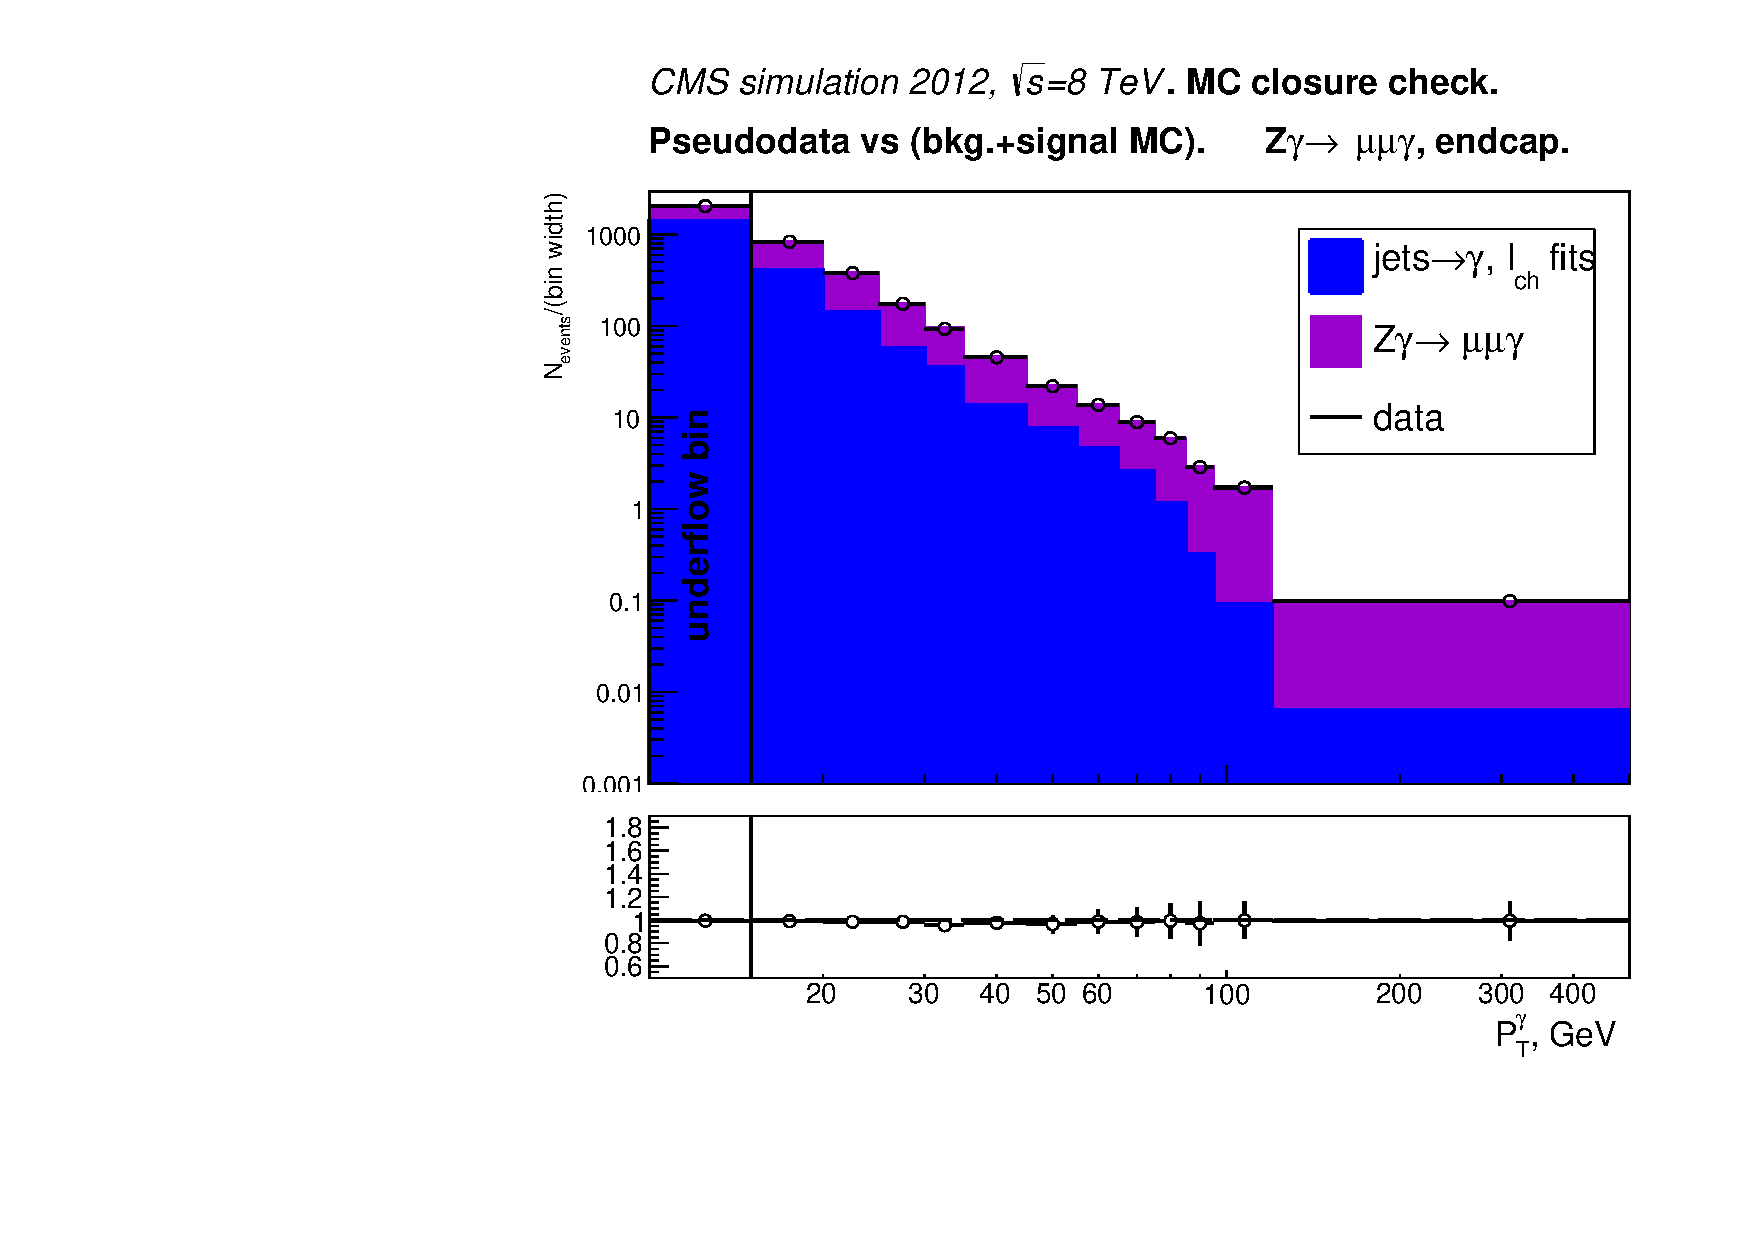
\includegraphics[width=0.45\textwidth]{../figs/figs_v11/MUON_ZGamma/PrepareYields/c_DATAvsBkgPlusSigMCc_MUON_ZGamma_TEMPL_CHISO_UNblind_MCclosure__Endcap__phoEt_MCclosure.pdf}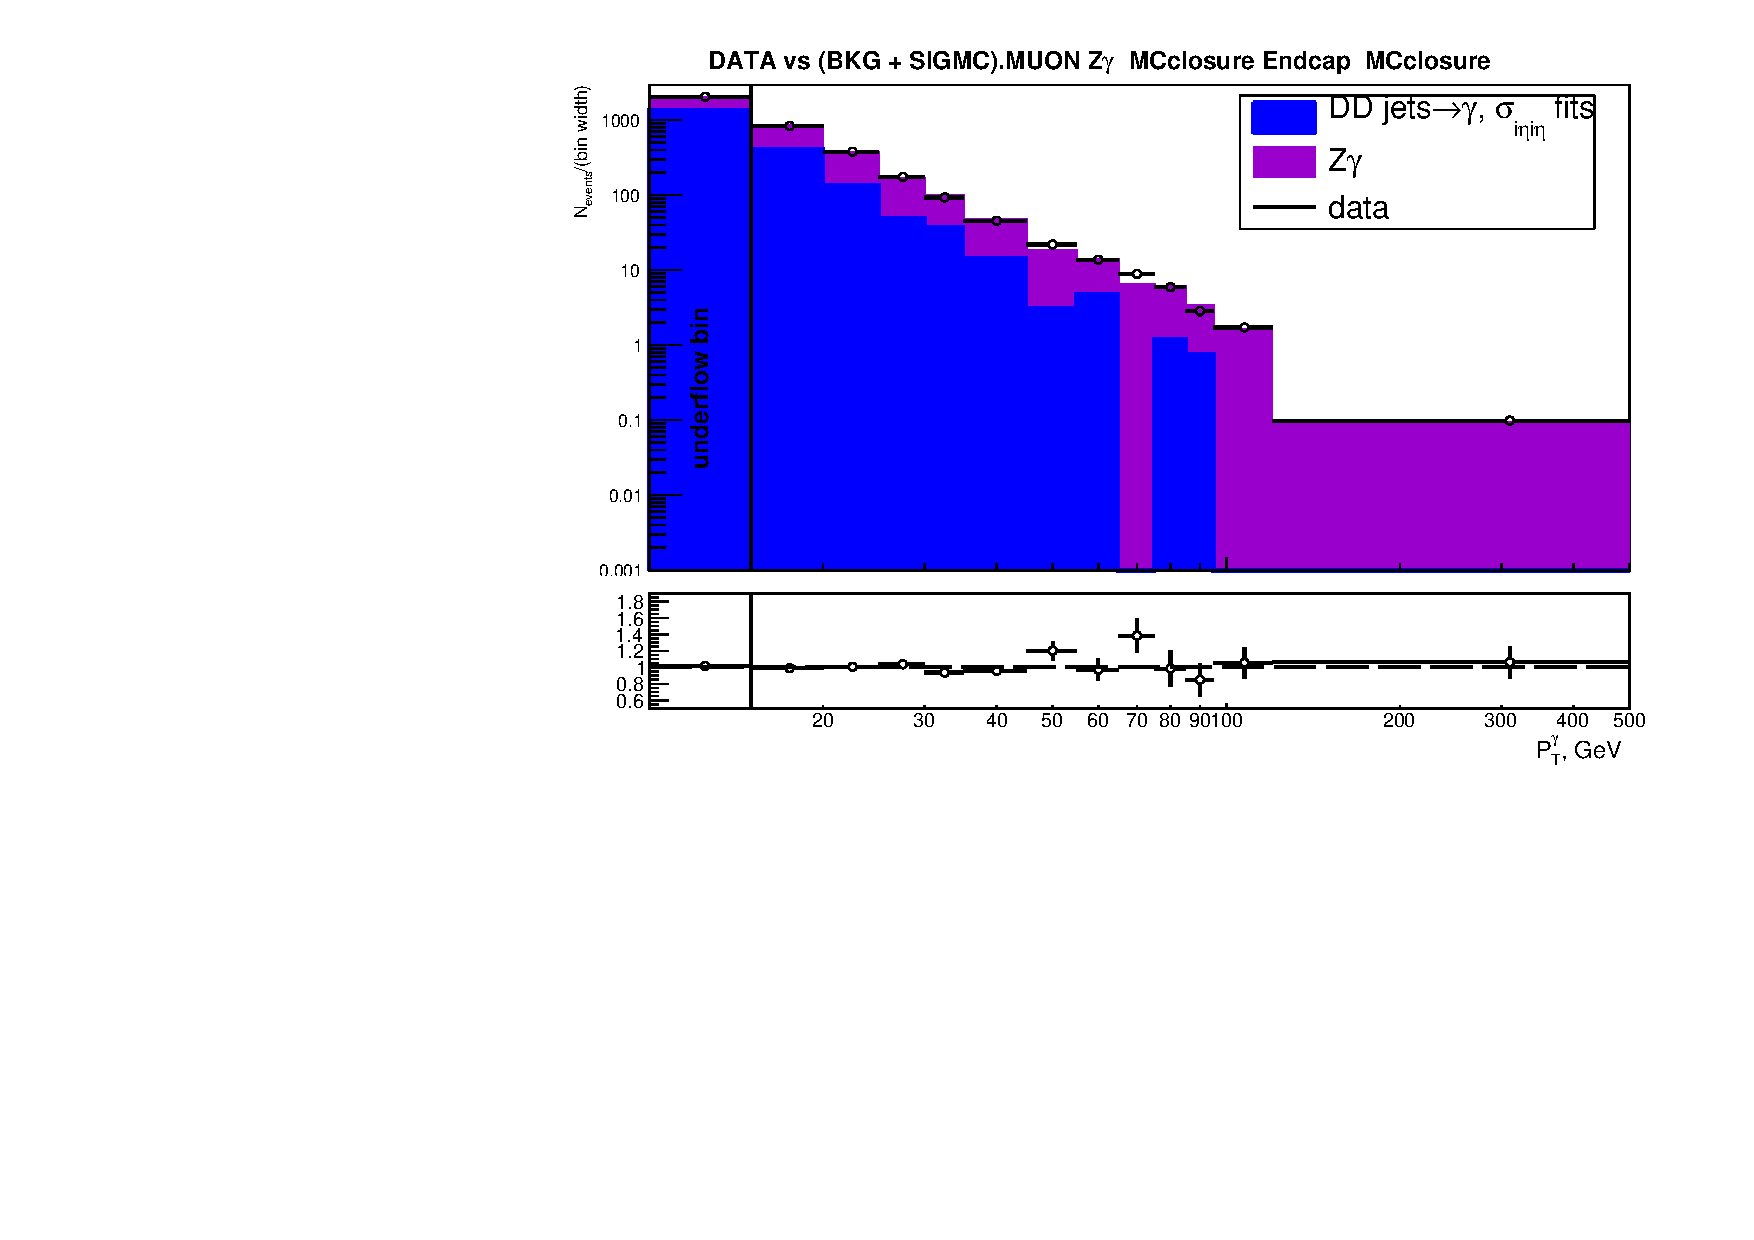
\includegraphics[width=0.45\textwidth]{../figs/figs_v11/MUON_ZGamma/PrepareYields/c_DATAvsBkgPlusSigMCc_MUON_ZGamma_TEMPL_SIHIH_UNblind_MCclosure__Endcap__phoEt_MCclosure.pdf}  \\
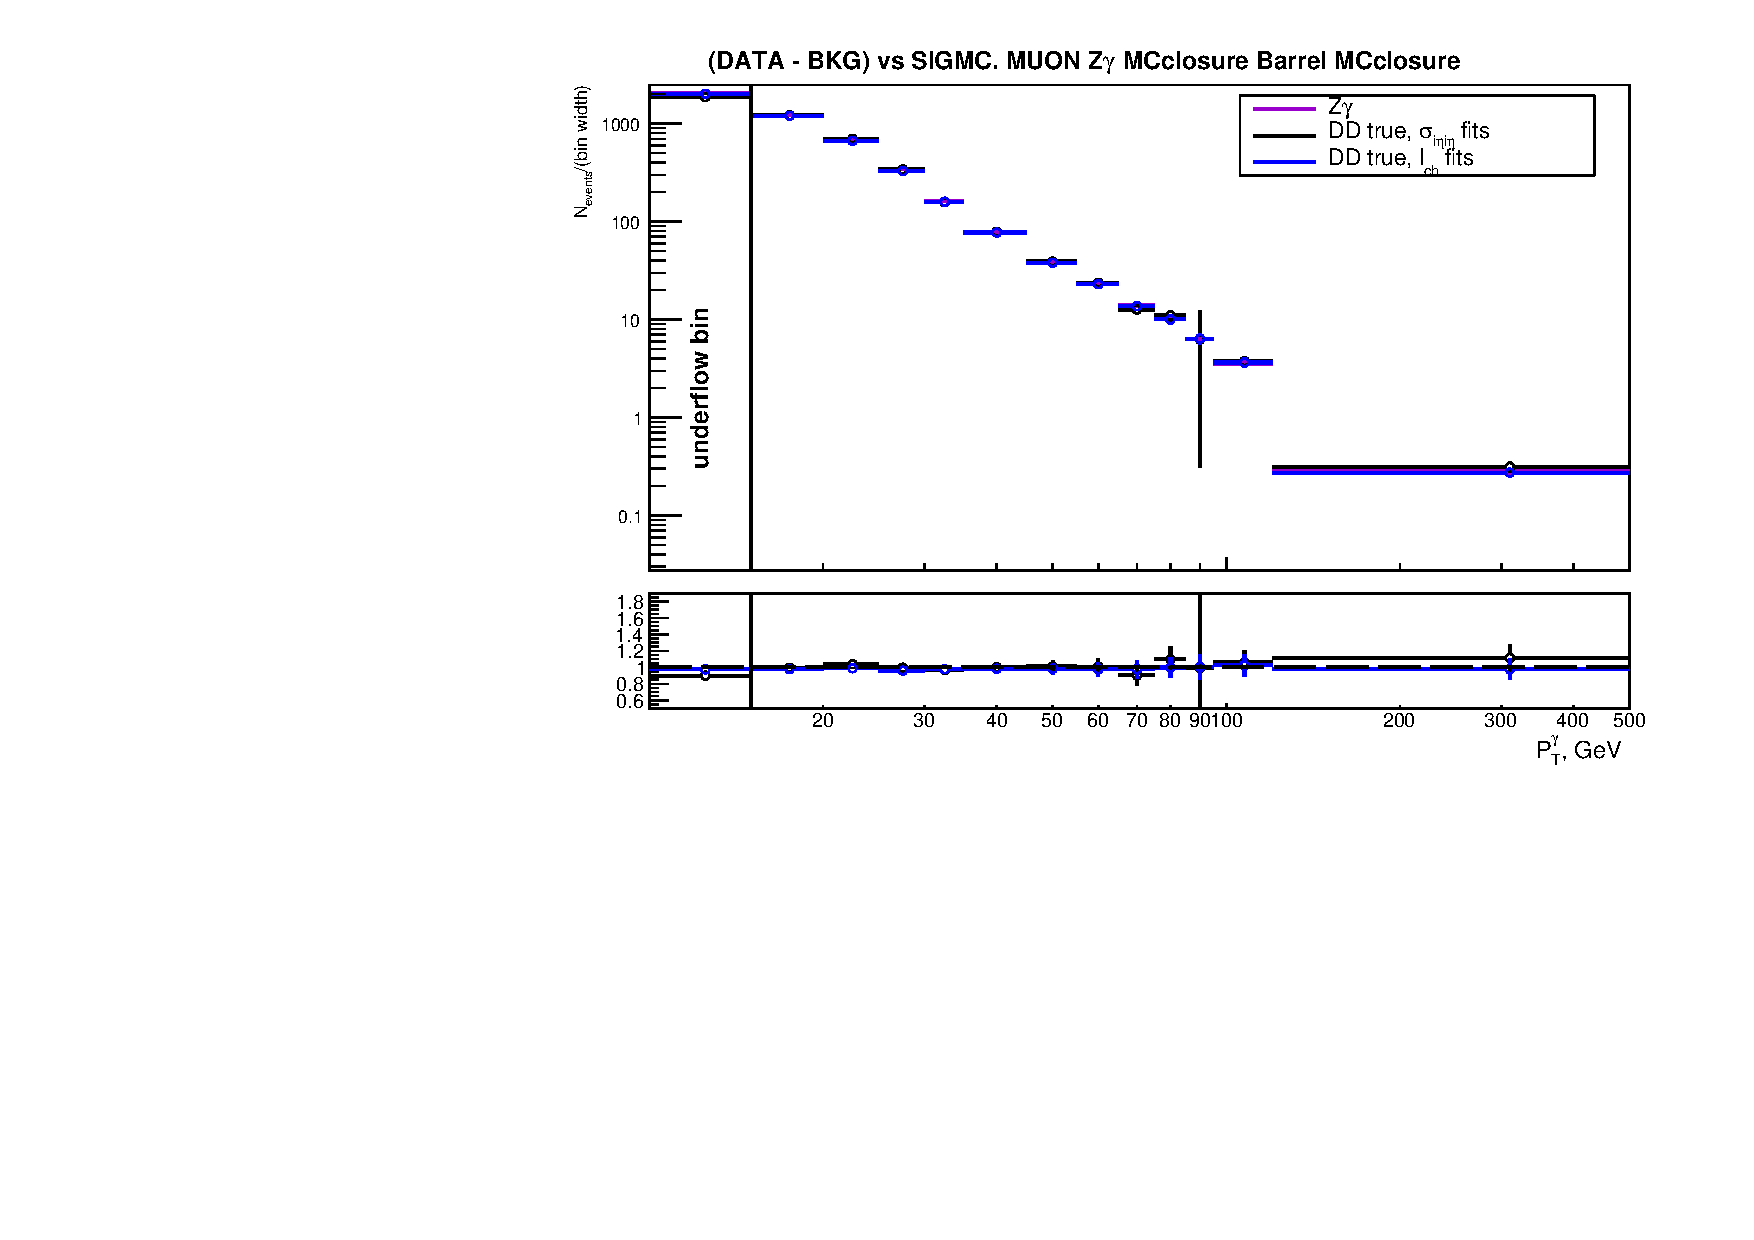
\includegraphics[width=0.45\textwidth]{../figs/figs_v11/MUON_ZGamma/PrepareYields/c_BkgSubtrDATAvsSIGMC_c_MUON_ZGamma__UNblind_MCclosure__Barrel__phoEt_MCclosure.pdf}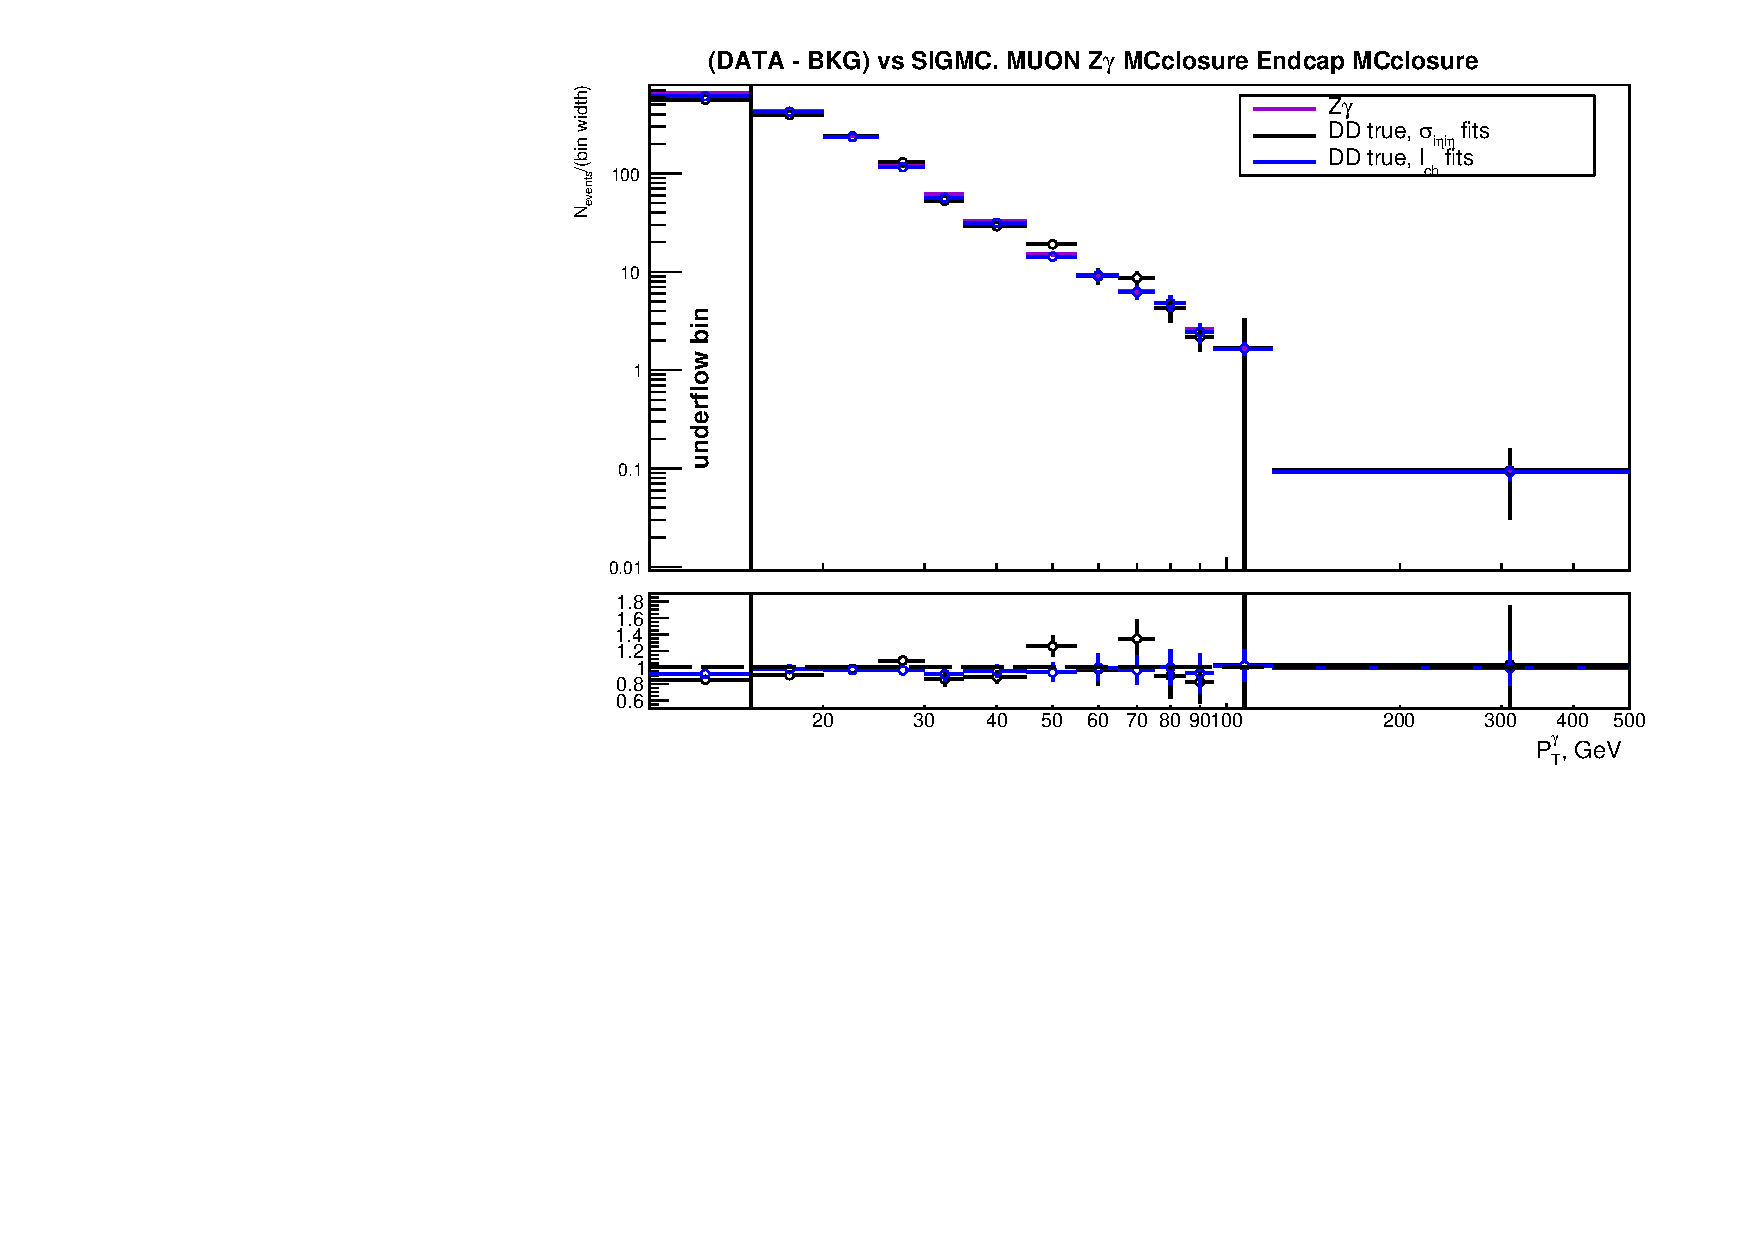
\includegraphics[width=0.45\textwidth]{../figs/figs_v11/MUON_ZGamma/PrepareYields/c_BkgSubtrDATAvsSIGMC_c_MUON_ZGamma__UNblind_MCclosure__Endcap__phoEt_MCclosure.pdf}\\
  \caption{$Z\gamma$ MC closure check. Muon channel. Top and middle: pseudodata vs fake-$\gamma$ background derived from the template method + real-$\gamma$ background predicted by dedicated MC samples + signal MC, with $I_{ch}$ and $\sigma_{i\etai\eta}$ used as fit variables. Bottom: pseudodata yields after full background subtraction vs signal MC. $I_{ch}$ vs $\sigma_{i\etai\eta}$ fit results. }
  \label{fig:DDvsMC_Zg_MCclosure_MUON}
  \end{center}
\end{figure}

\begin{figure}[htb]
  \begin{center}
   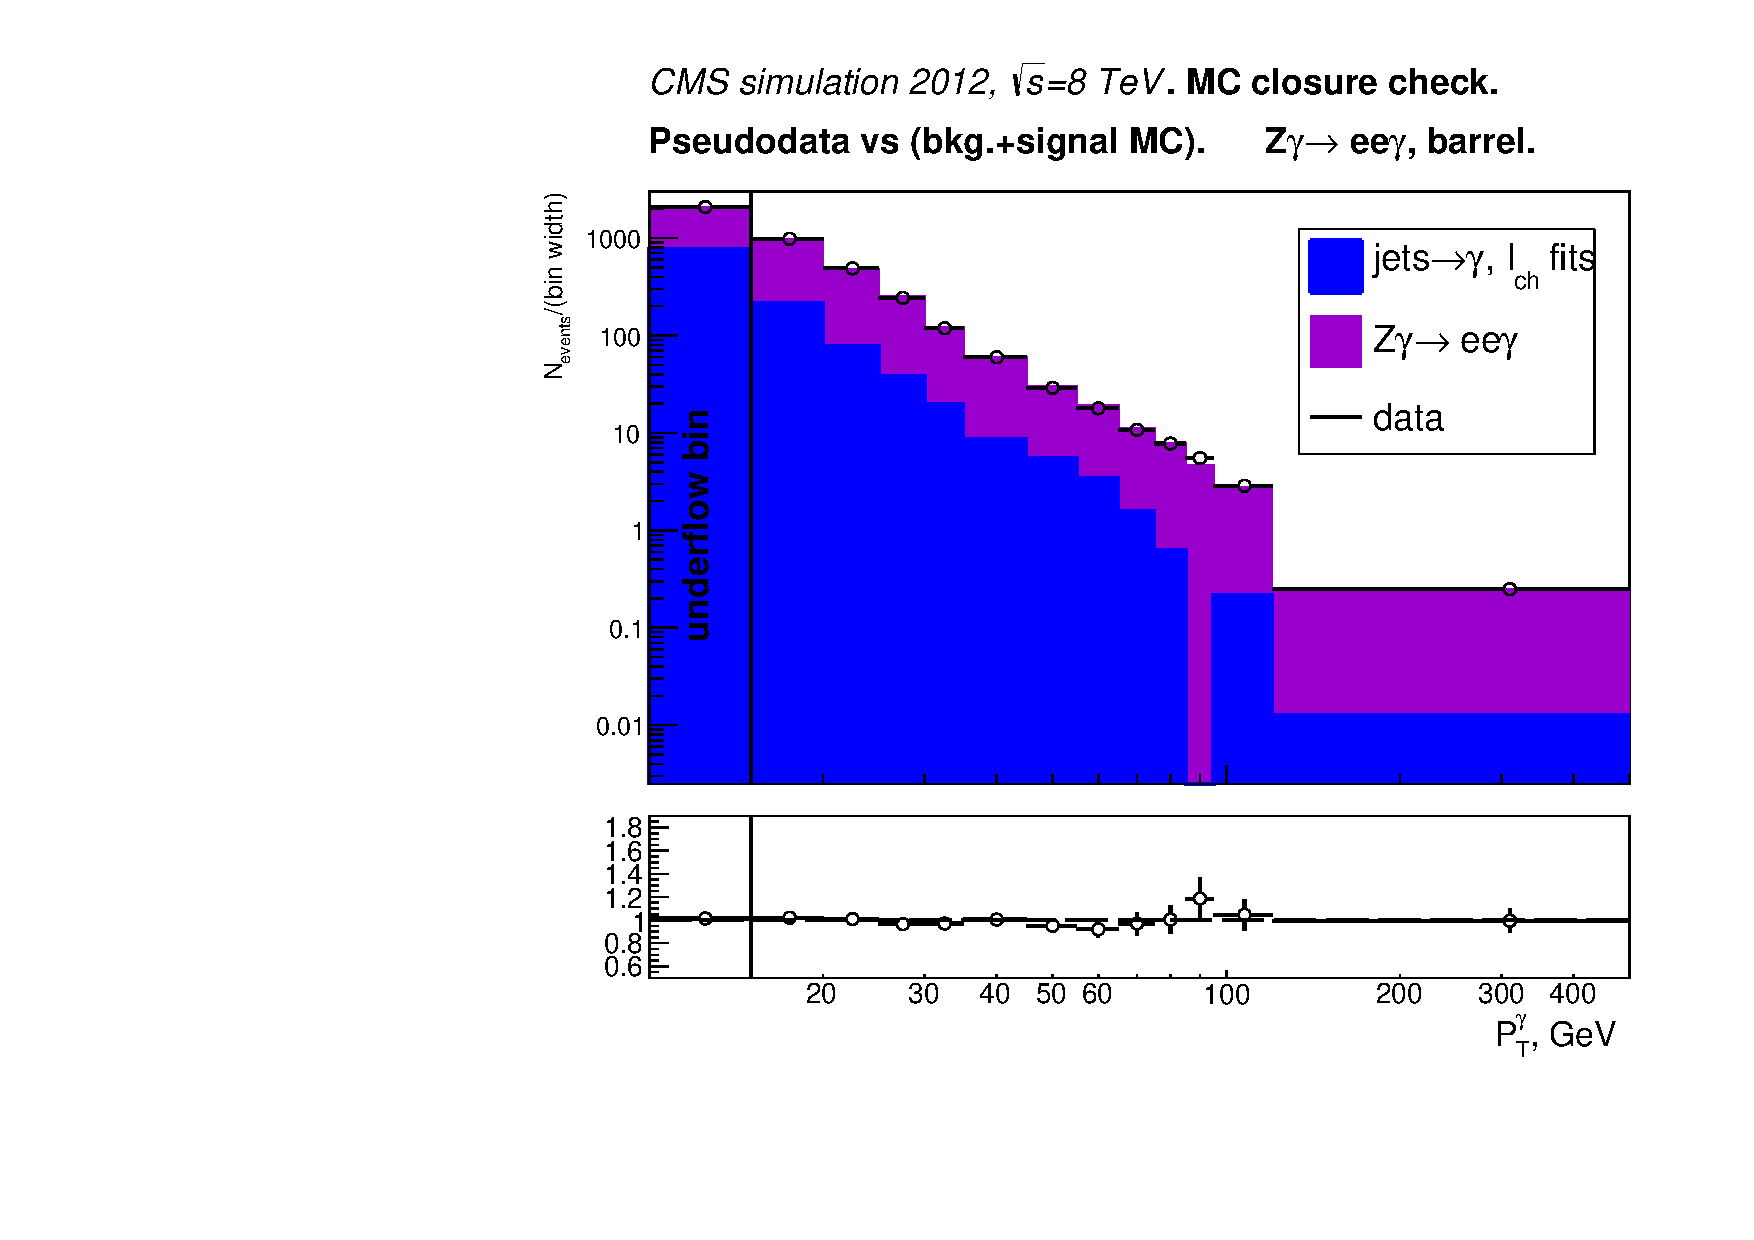
\includegraphics[width=0.45\textwidth]{../figs/figs_v11/ELECTRON_ZGamma/PrepareYields/c_DATAvsBkgPlusSigMCc_ELECTRON_ZGamma_TEMPL_CHISO_UNblind_MCclosure__Barrel__phoEt_MCclosure.pdf}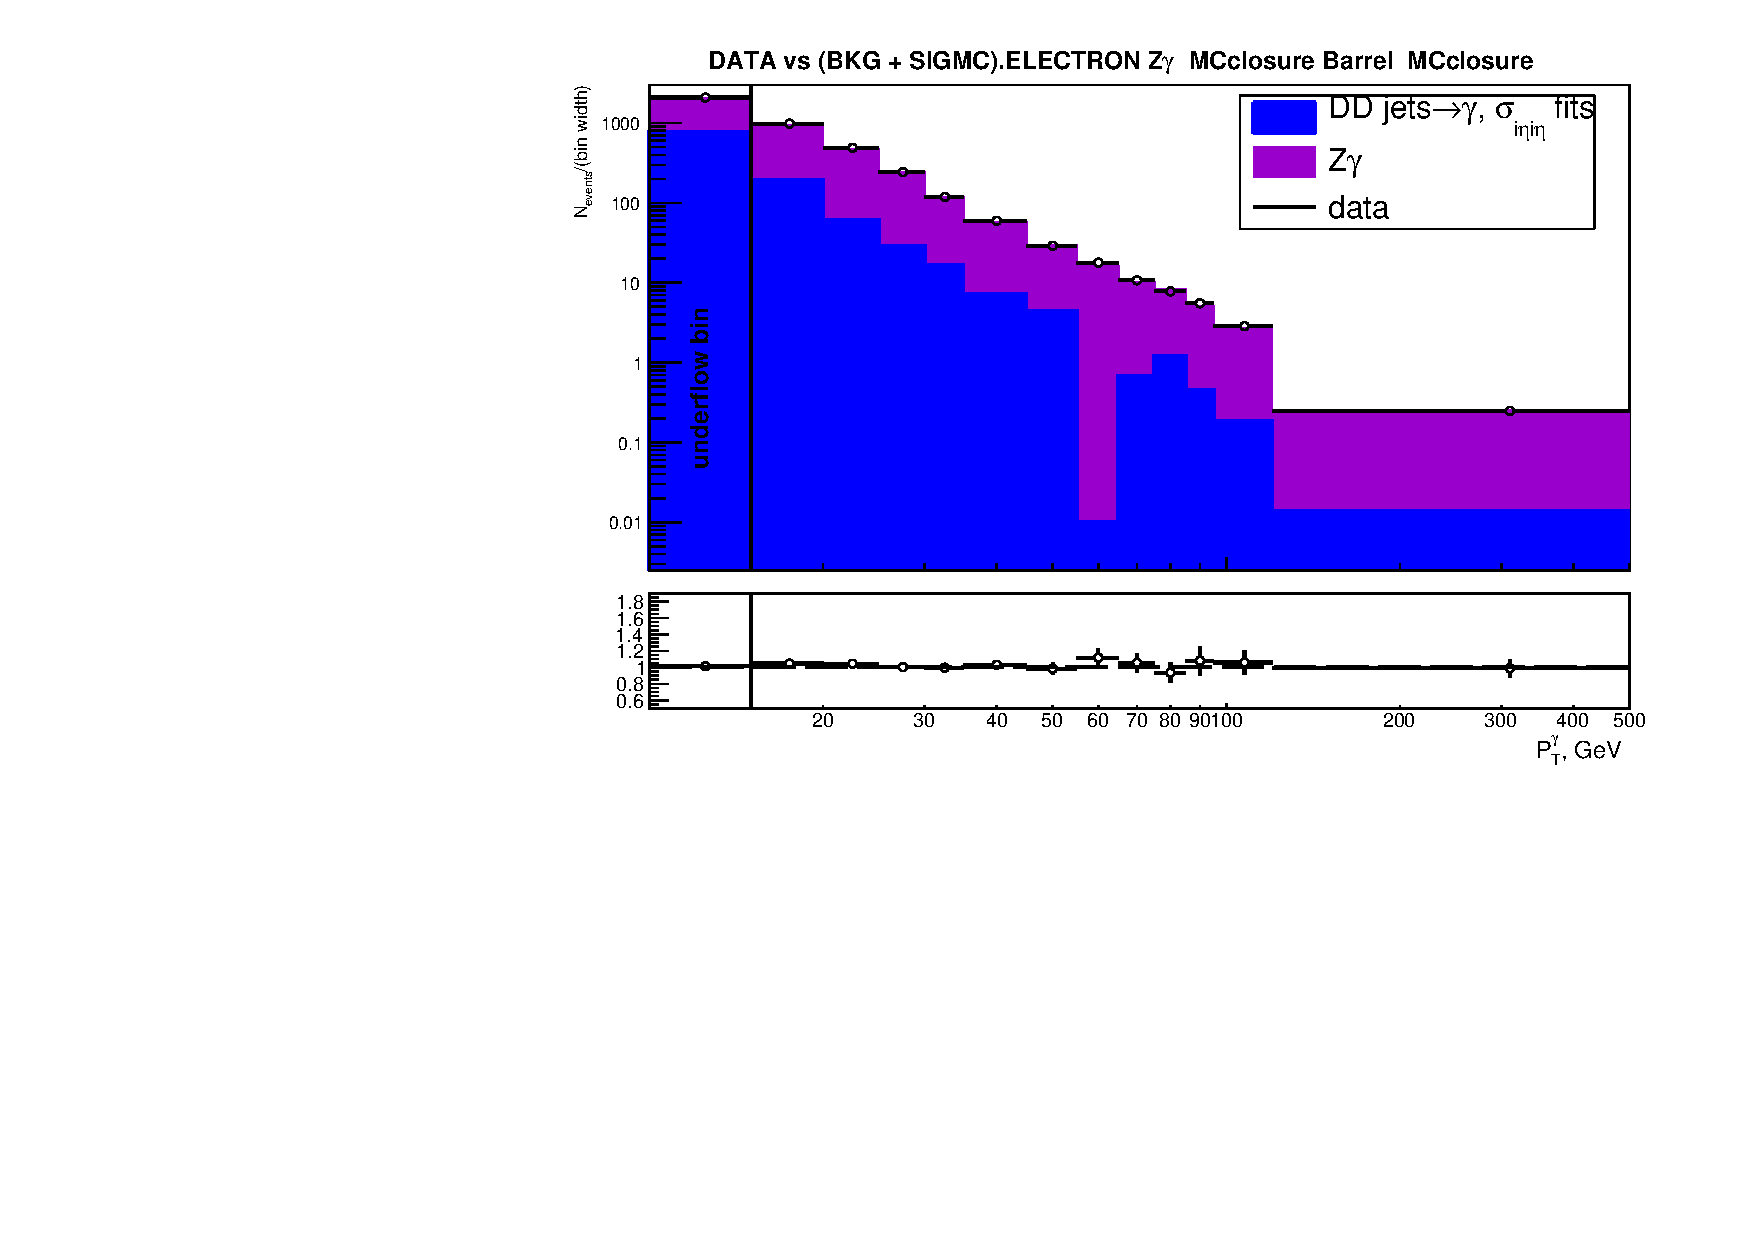
\includegraphics[width=0.45\textwidth]{../figs/figs_v11/ELECTRON_ZGamma/PrepareYields/c_DATAvsBkgPlusSigMCc_ELECTRON_ZGamma_TEMPL_SIHIH_UNblind_MCclosure__Barrel__phoEt_MCclosure.pdf}  \\
   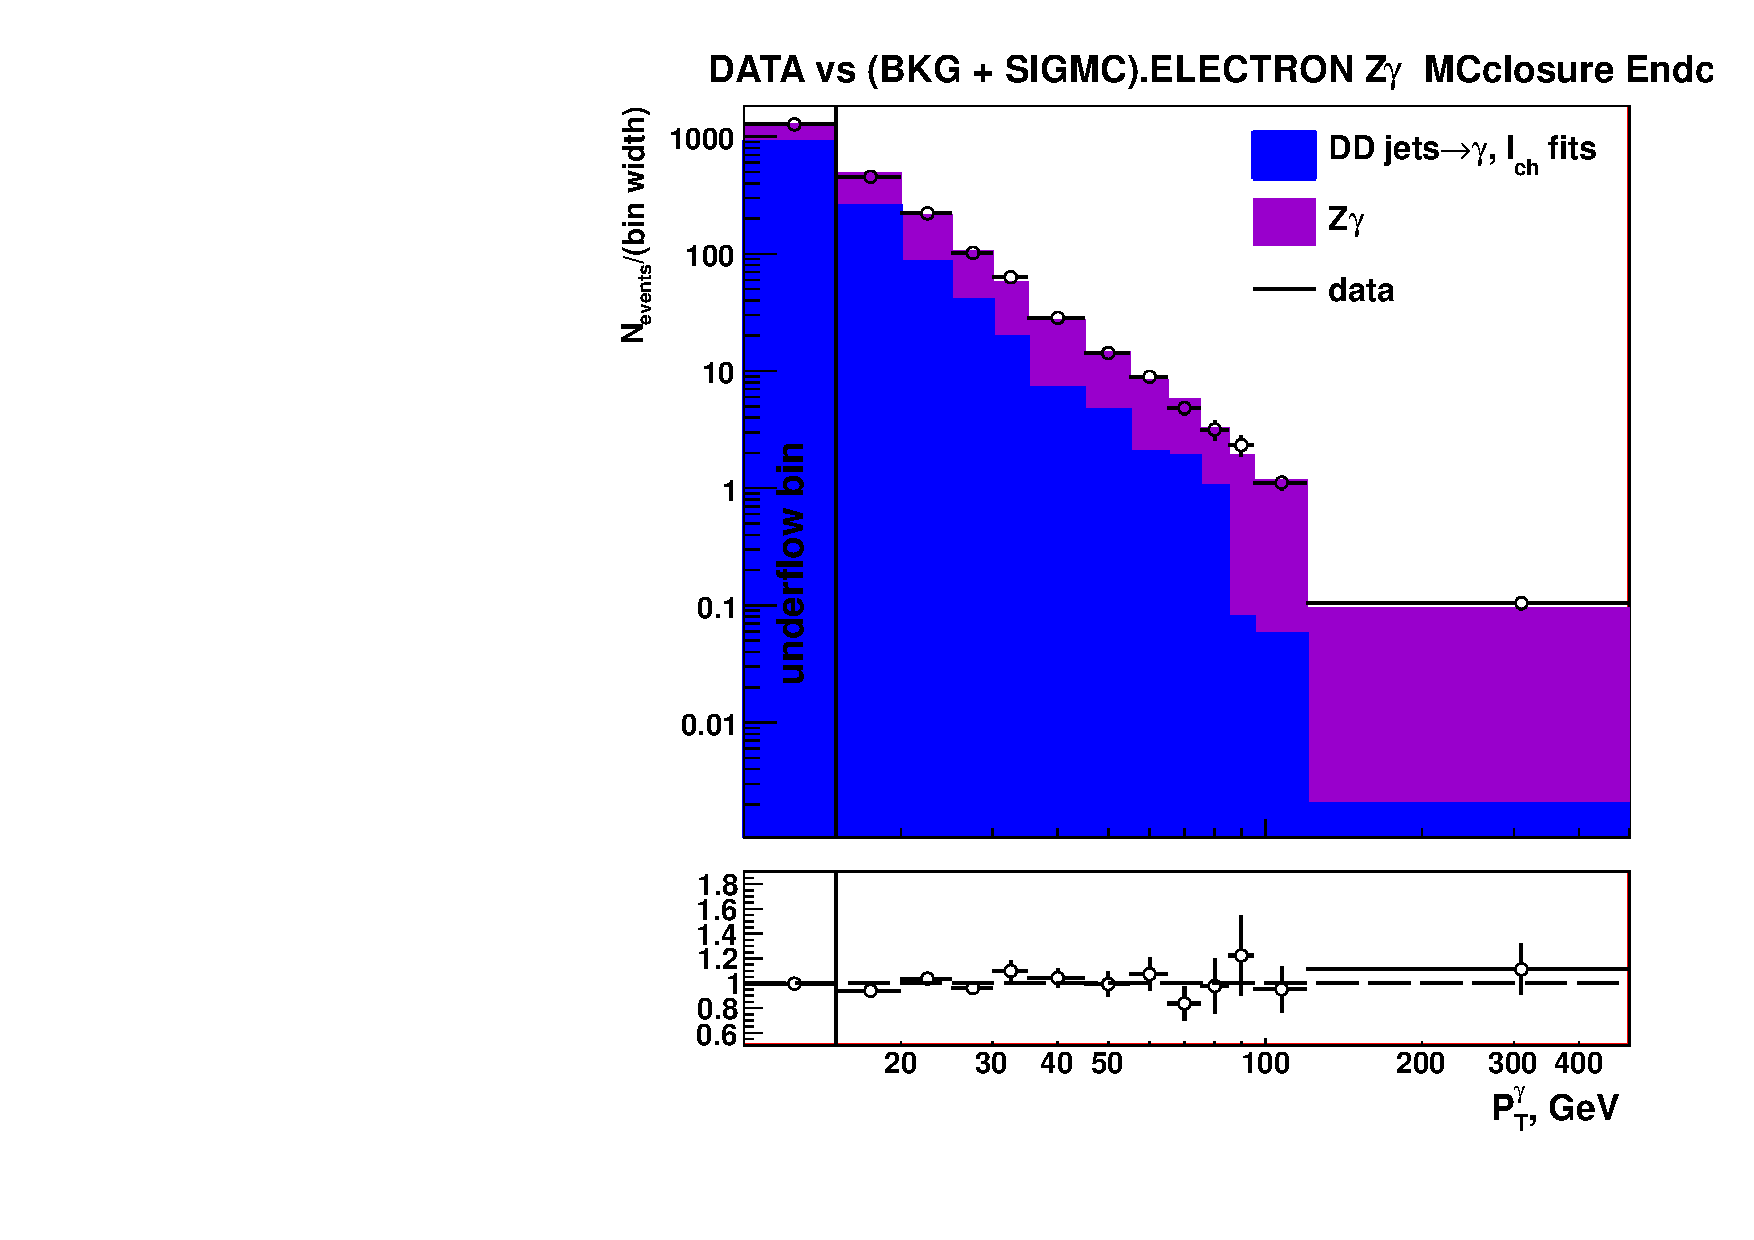
\includegraphics[width=0.45\textwidth]{../figs/figs_v11/ELECTRON_ZGamma/PrepareYields/c_DATAvsBkgPlusSigMCc_ELECTRON_ZGamma_TEMPL_CHISO_UNblind_MCclosure__Endcap__phoEt_MCclosure.pdf}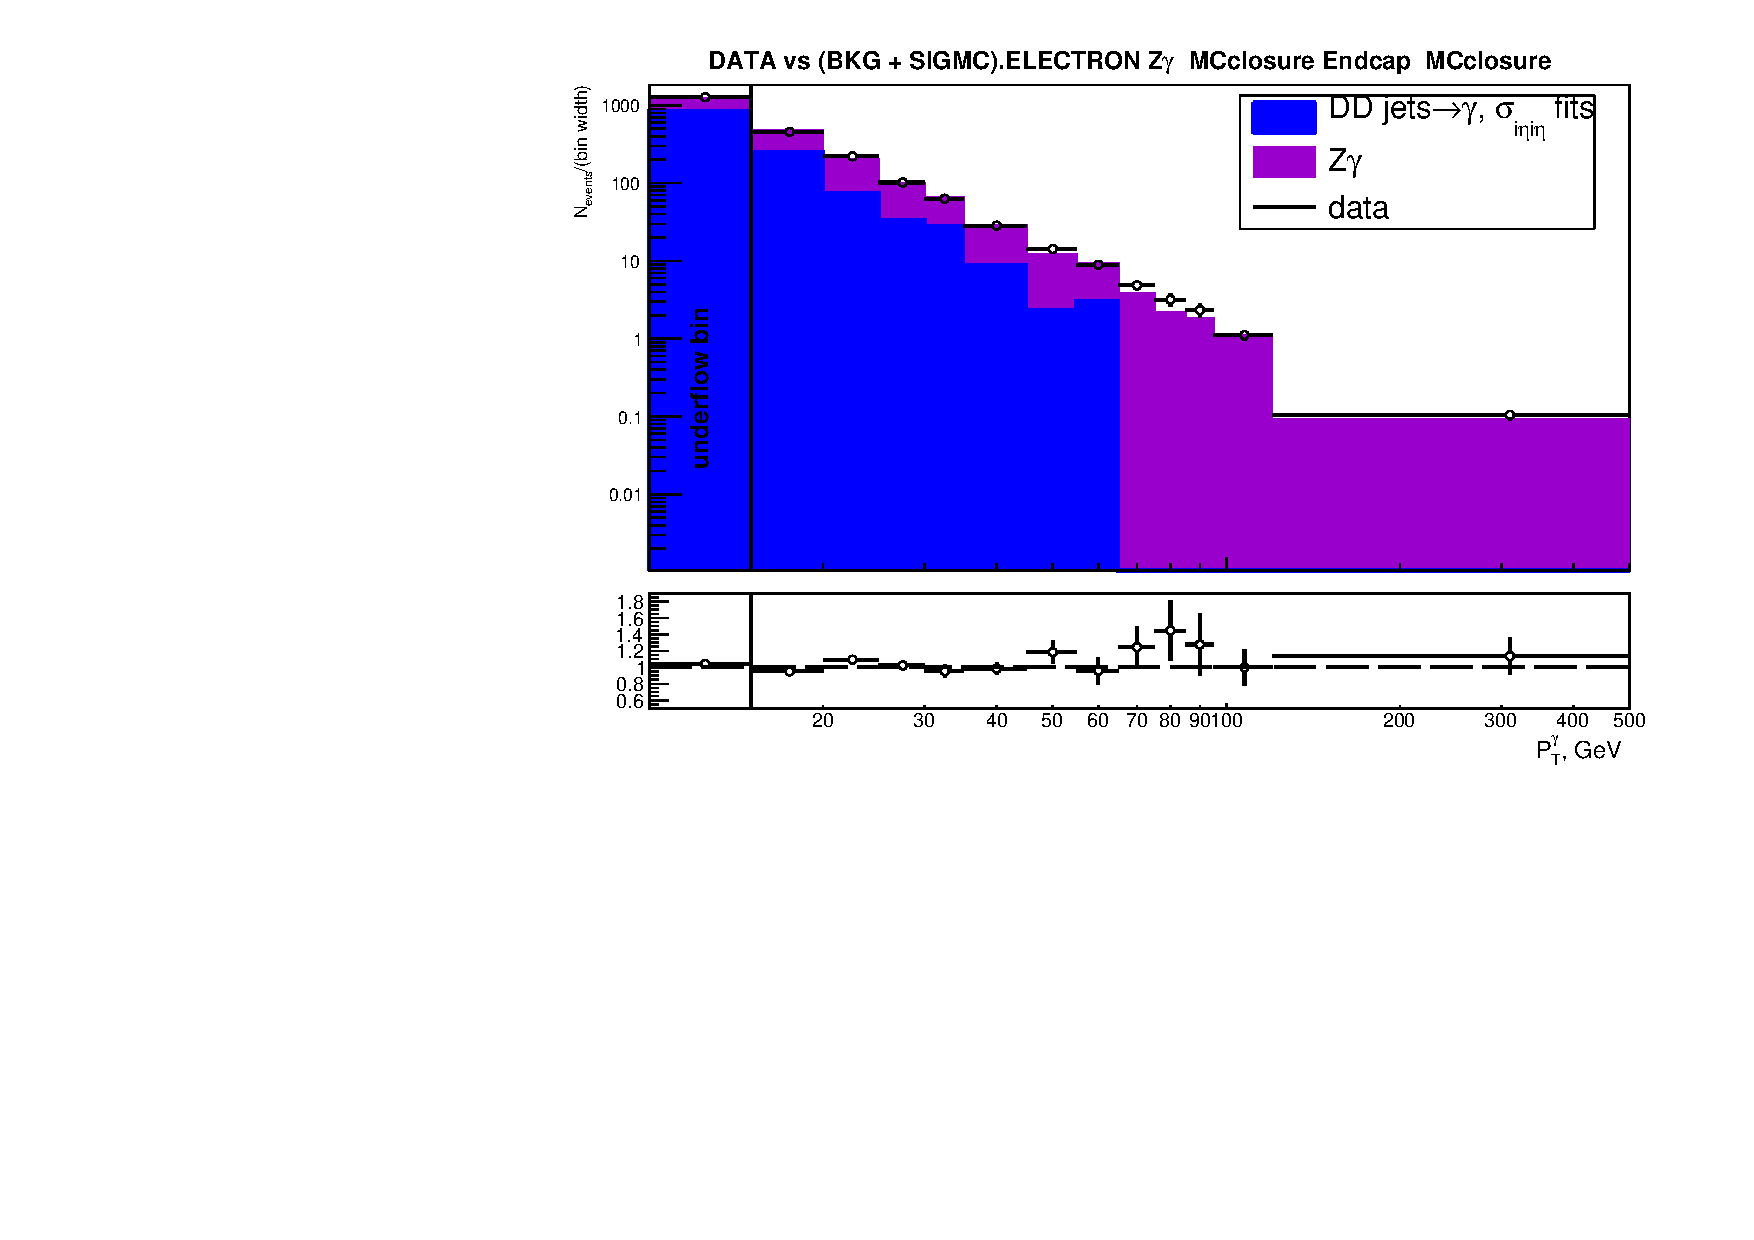
\includegraphics[width=0.45\textwidth]{../figs/figs_v11/ELECTRON_ZGamma/PrepareYields/c_DATAvsBkgPlusSigMCc_ELECTRON_ZGamma_TEMPL_SIHIH_UNblind_MCclosure__Endcap__phoEt_MCclosure.pdf}  \\
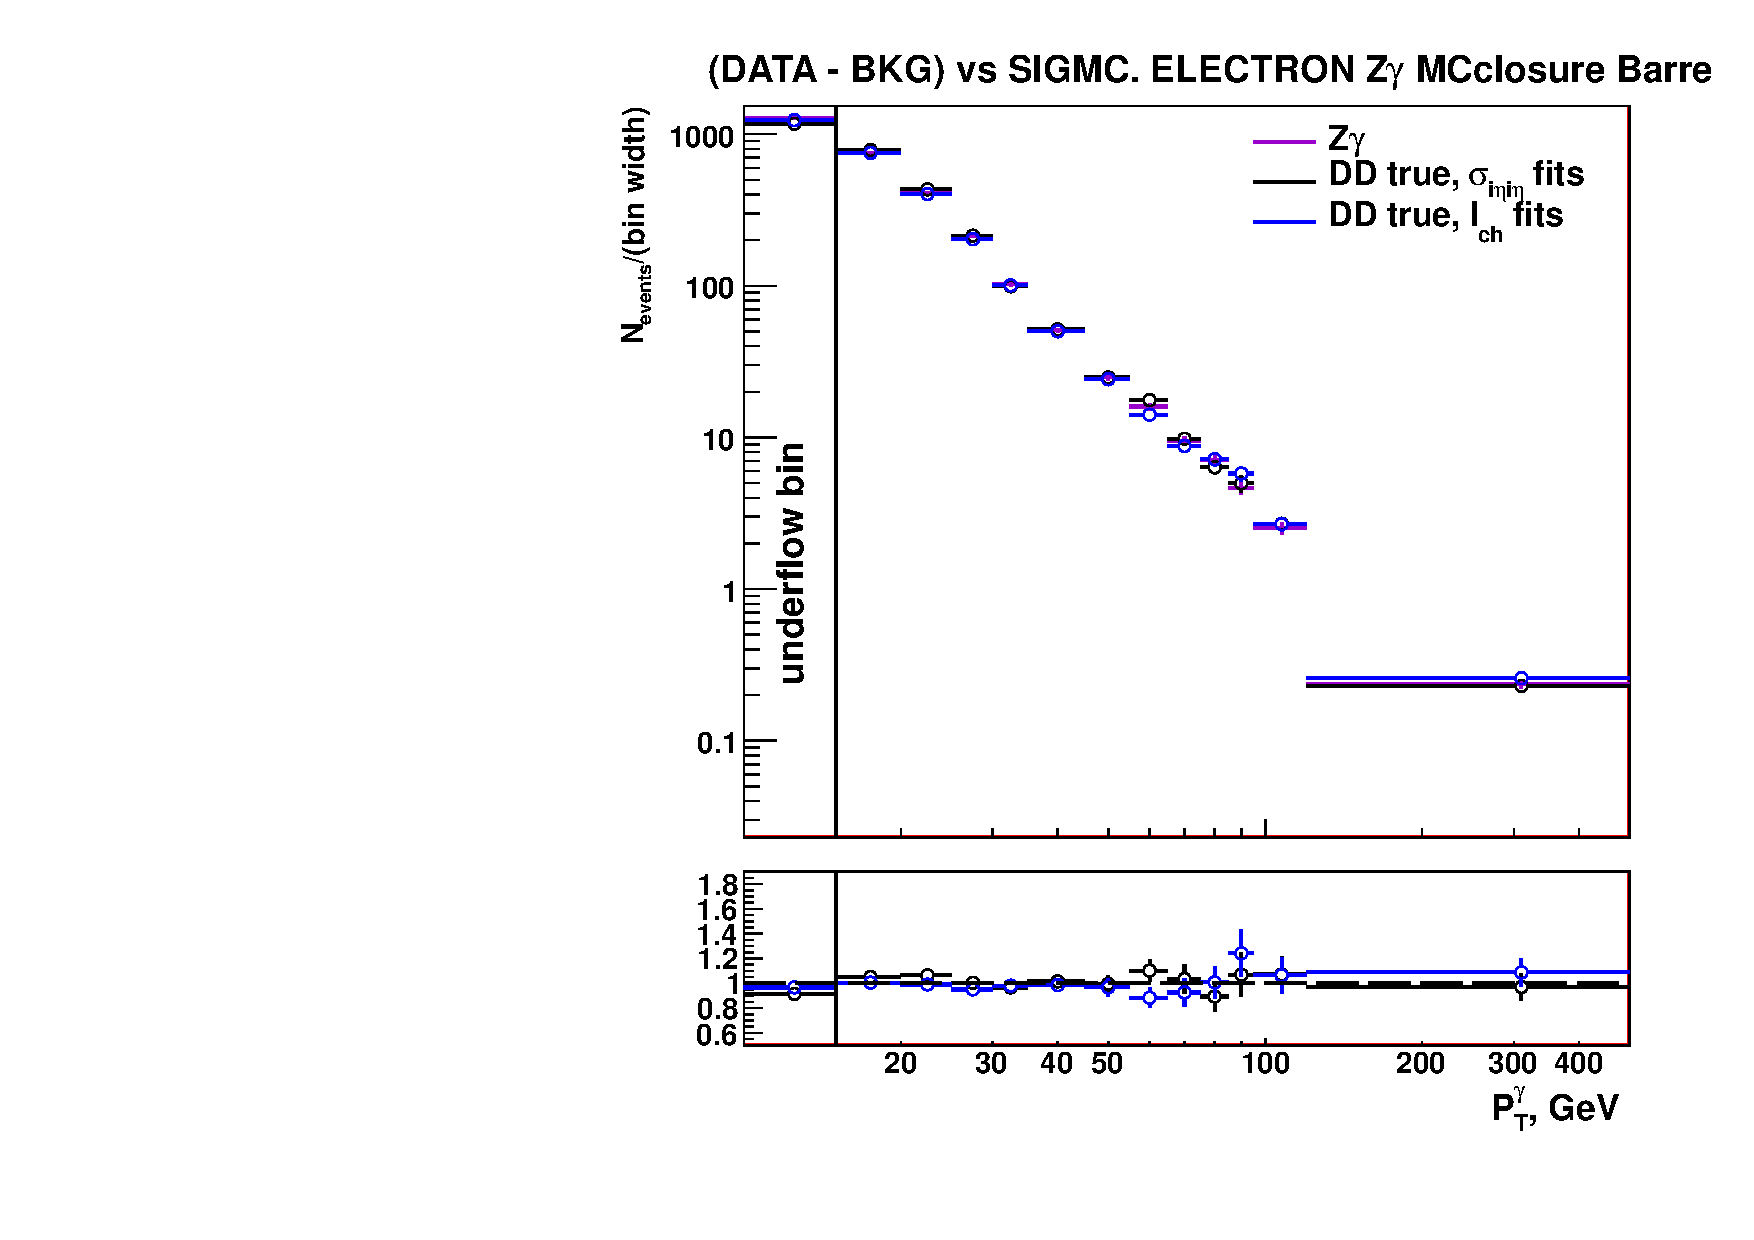
\includegraphics[width=0.45\textwidth]{../figs/figs_v11/ELECTRON_ZGamma/PrepareYields/c_BkgSubtrDATAvsSIGMC_c_ELECTRON_ZGamma__UNblind_MCclosure__Barrel__phoEt_MCclosure.pdf}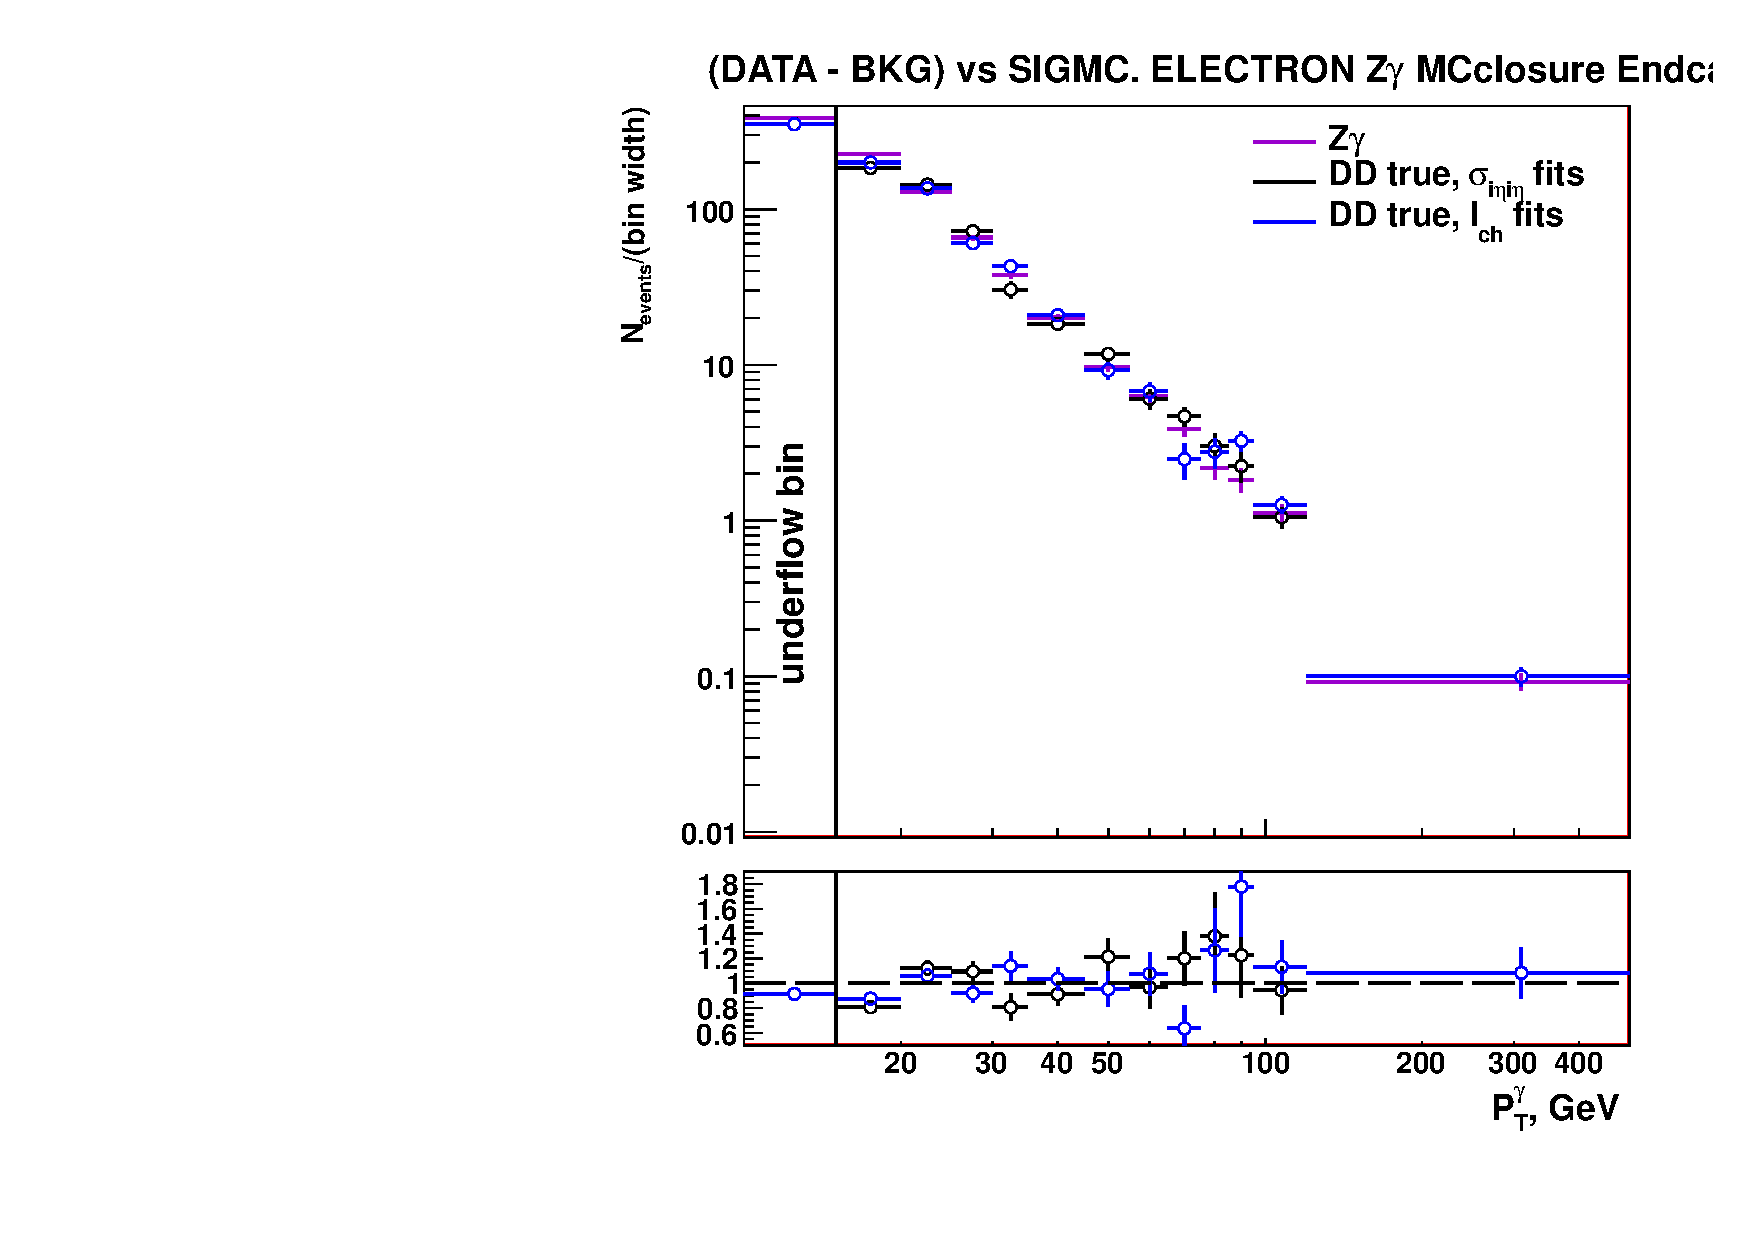
\includegraphics[width=0.45\textwidth]{../figs/figs_v11/ELECTRON_ZGamma/PrepareYields/c_BkgSubtrDATAvsSIGMC_c_ELECTRON_ZGamma__UNblind_MCclosure__Endcap__phoEt_MCclosure.pdf}\\
  \caption{$Z\gamma$ MC closure check. Electron channel. Top and middle: pseudodata vs fake-$\gamma$ background derived from the template method + real-$\gamma$ background predicted by dedicated MC samples + signal MC, with $I_{ch}$ and $\sigma_{i\etai\eta}$ used as fit variables. Bottom: pseudodata yields after full background subtraction vs signal MC. $I_{ch}$ vs $\sigma_{i\etai\eta}$ fit results. }
  \label{fig:DDvsMC_Zg_MCclosure_ELECTRON}
  \end{center}
\end{figure}

\clearpage

\begin{table}[h]
  \scriptsize
  \begin{center}
  \caption{Relative errors [\%]. MUON $Z\gamma$}
  \begin{tabular}{|c|c|c|c|c|c|c|c|c|}
    bin  & err & syst & $Z\gamma$ MC & $A \times \epsilon$ & syst & unf & syst & syst + stat\\
    lims  & stat & $|N_{Ich}-N_{\sigma{i\eta i\eta}}|$ & norm & MC stat & lumi & MC stat & total & total\\ \hline
    total  & 1 & 1 & 1 & 0 & 3 & 1 & 3 & 3 \\ \hline
%    10-15 & 2 & 3 & 3 & 1 & 3 & 2 & 5 & 5 \\ \hline
    15-20 & 2 & 2 & 2 & 1 & 3 & 2 & 4 & 5 \\ \hline
    20-25 & 2 & 2 & 3 & 1 & 3 & 2 & 5 & 5 \\ \hline
    25-30 & 3 & 3 & 4 & 2 & 3 & 3 & 7 & 8 \\ \hline
    30-35 & 4 & 6 & 5 & 3 & 3 & 5 & 10 & 10 \\ \hline
    35-45 & 4 & 3 & 6 & 3 & 3 & 4 & 9 & 9 \\ \hline
    45-55 & 6 & 8 & 8 & 4 & 3 & 6 & 14 & 15 \\ \hline
    55-65 & 7 & 5 & 7 & 5 & 3 & 7 & 13 & 14 \\ \hline
    65-75 & 9 & 7 & 8 & 6 & 3 & 9 & 16 & 18 \\ \hline
    75-85 & 10 & 8 & 6 & 7 & 3 & 10 & 16 & 19 \\ \hline
    85-95 & 12 & 8 & 8 & 9 & 3 & 12 & 19 & 23 \\ \hline
    95-120 & 11 & 10 & 6 & 8 & 3 & 11 & 18 & 21 \\ \hline
    120-500 & 8 & 5 & 9 & 7 & 3 & 9 & 16 & 18 \\ \hline
  \end{tabular}
  \label{tab:systInPercent_MUON_ZGamma}
  \end{center}
\end{table}

\begin{table}[h]
  \scriptsize
  \begin{center}
  \caption{Relative errors [\%]. ELECTRON $Z\gamma$}
  \begin{tabular}{|c|c|c|c|c|c|c|c|c|}
    bin  & err & syst & $Z\gamma$ MC & $A\times \epsilon$ & syst & unf & syst & syst + stat\\
    lims  & stat & $|N_{Ich}-N_{\sigma{i\eta i\eta}}|$ & norm & MC stat & lumi & MC stat & total & total\\ \hline
    total  & 1 & 1 & 1 & 0 & 3 & 1 & 3 & 4 \\ \hline
%    10-15 & 2 & 2 & 3 & 1 & 3 & 2 & 5 & 5 \\ \hline
    15-20 & 2 & 3 & 3 & 1 & 3 & 2 & 5 & 6 \\ \hline
    20-25 & 3 & 2 & 3 & 1 & 3 & 3 & 5 & 6 \\ \hline
    25-30 & 4 & 3 & 4 & 2 & 3 & 4 & 7 & 8 \\ \hline
    30-35 & 5 & 4 & 5 & 3 & 3 & 6 & 10 & 11 \\ \hline
    35-45 & 5 & 4 & 6 & 3 & 3 & 5 & 10 & 11 \\ \hline
    45-55 & 6 & 6 & 6 & 4 & 3 & 7 & 11 & 13 \\ \hline
    55-65 & 9 & 7 & 8 & 5 & 3 & 9 & 15 & 17 \\ \hline
    65-75 & 10 & 8 & 8 & 7 & 3 & 11 & 18 & 20 \\ \hline
    75-85 & 14 & 11 & 12 & 9 & 3 & 16 & 25 & 28 \\ \hline
    85-95 & 15 & 9 & 6 & 10 & 3 & 17 & 23 & 28 \\ \hline
    95-120 & 10 & 5 & 6 & 9 & 3 & 11 & 16 & 19 \\ \hline
    120-500 & 9 & 3 & 7 & 8 & 3 & 10 & 15 & 17 \\ \hline
  \end{tabular}
  \label{tab:systInPercent_ELECTRON_ZGamma}
  \end{center}
\end{table}

\begin{figure}[htb]
  \begin{center}
   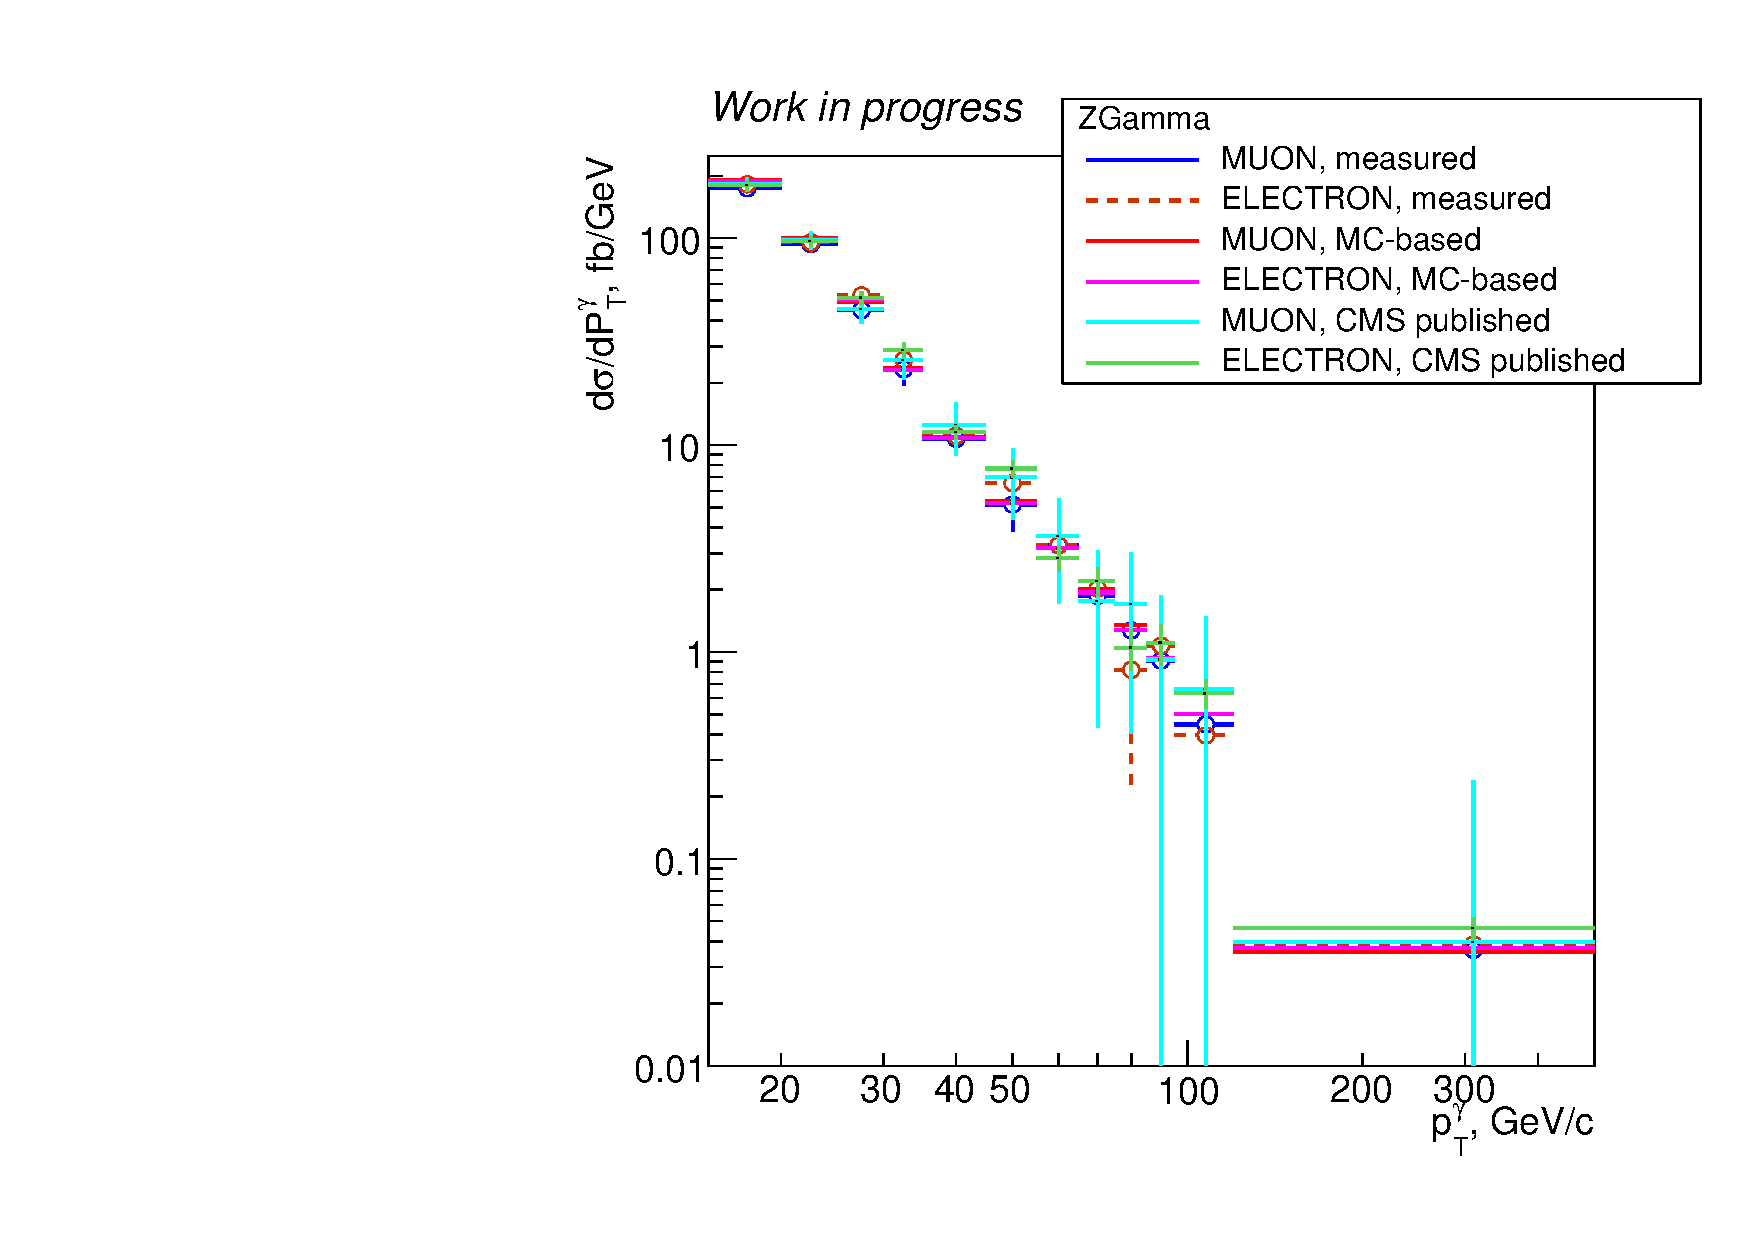
\includegraphics[width=0.33\textwidth]{../figs/figs_v11/ChannelsMERGED_ZGamma/CrossSection/compareCSZGamma.pdf}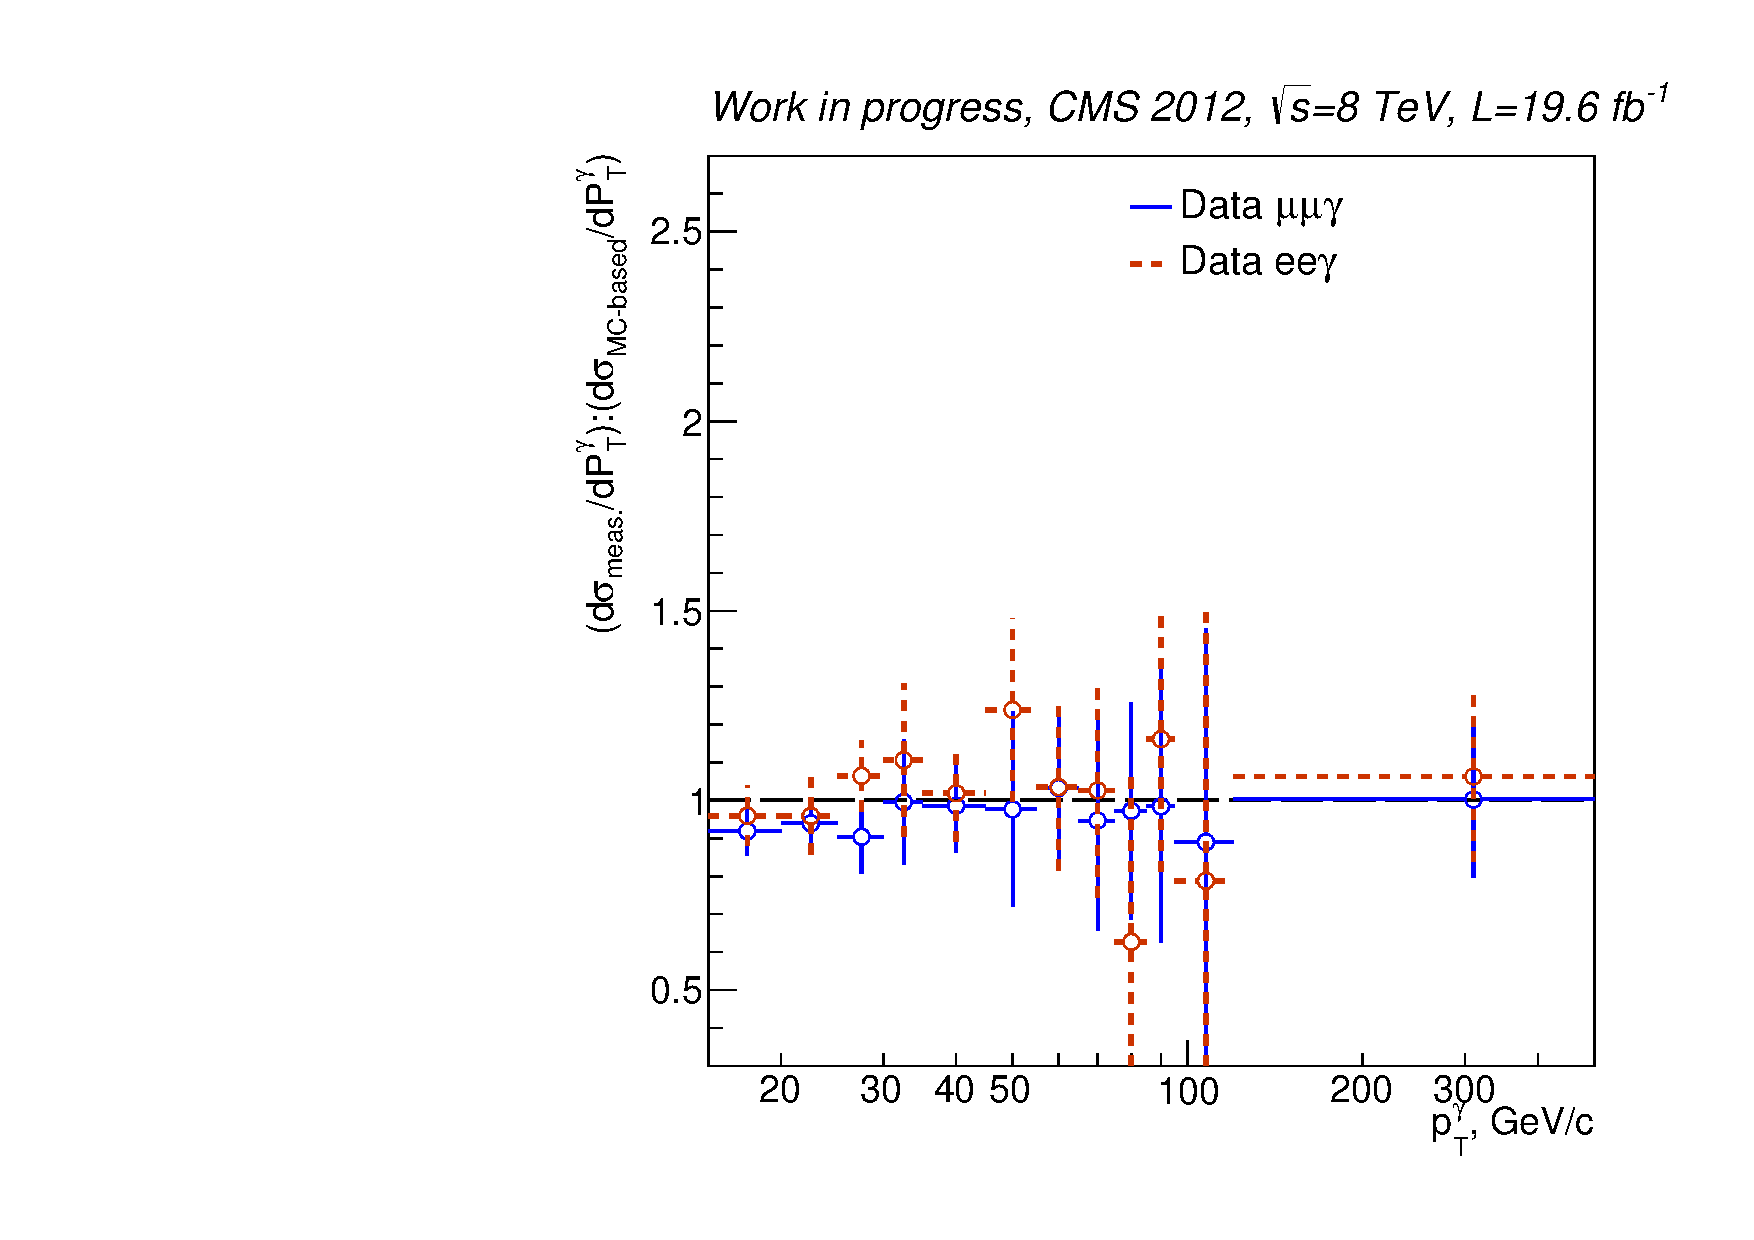
\includegraphics[width=0.33\textwidth]{../figs/figs_v11/ChannelsMERGED_ZGamma/CrossSection/compareCSratioTheoryZGamma.pdf}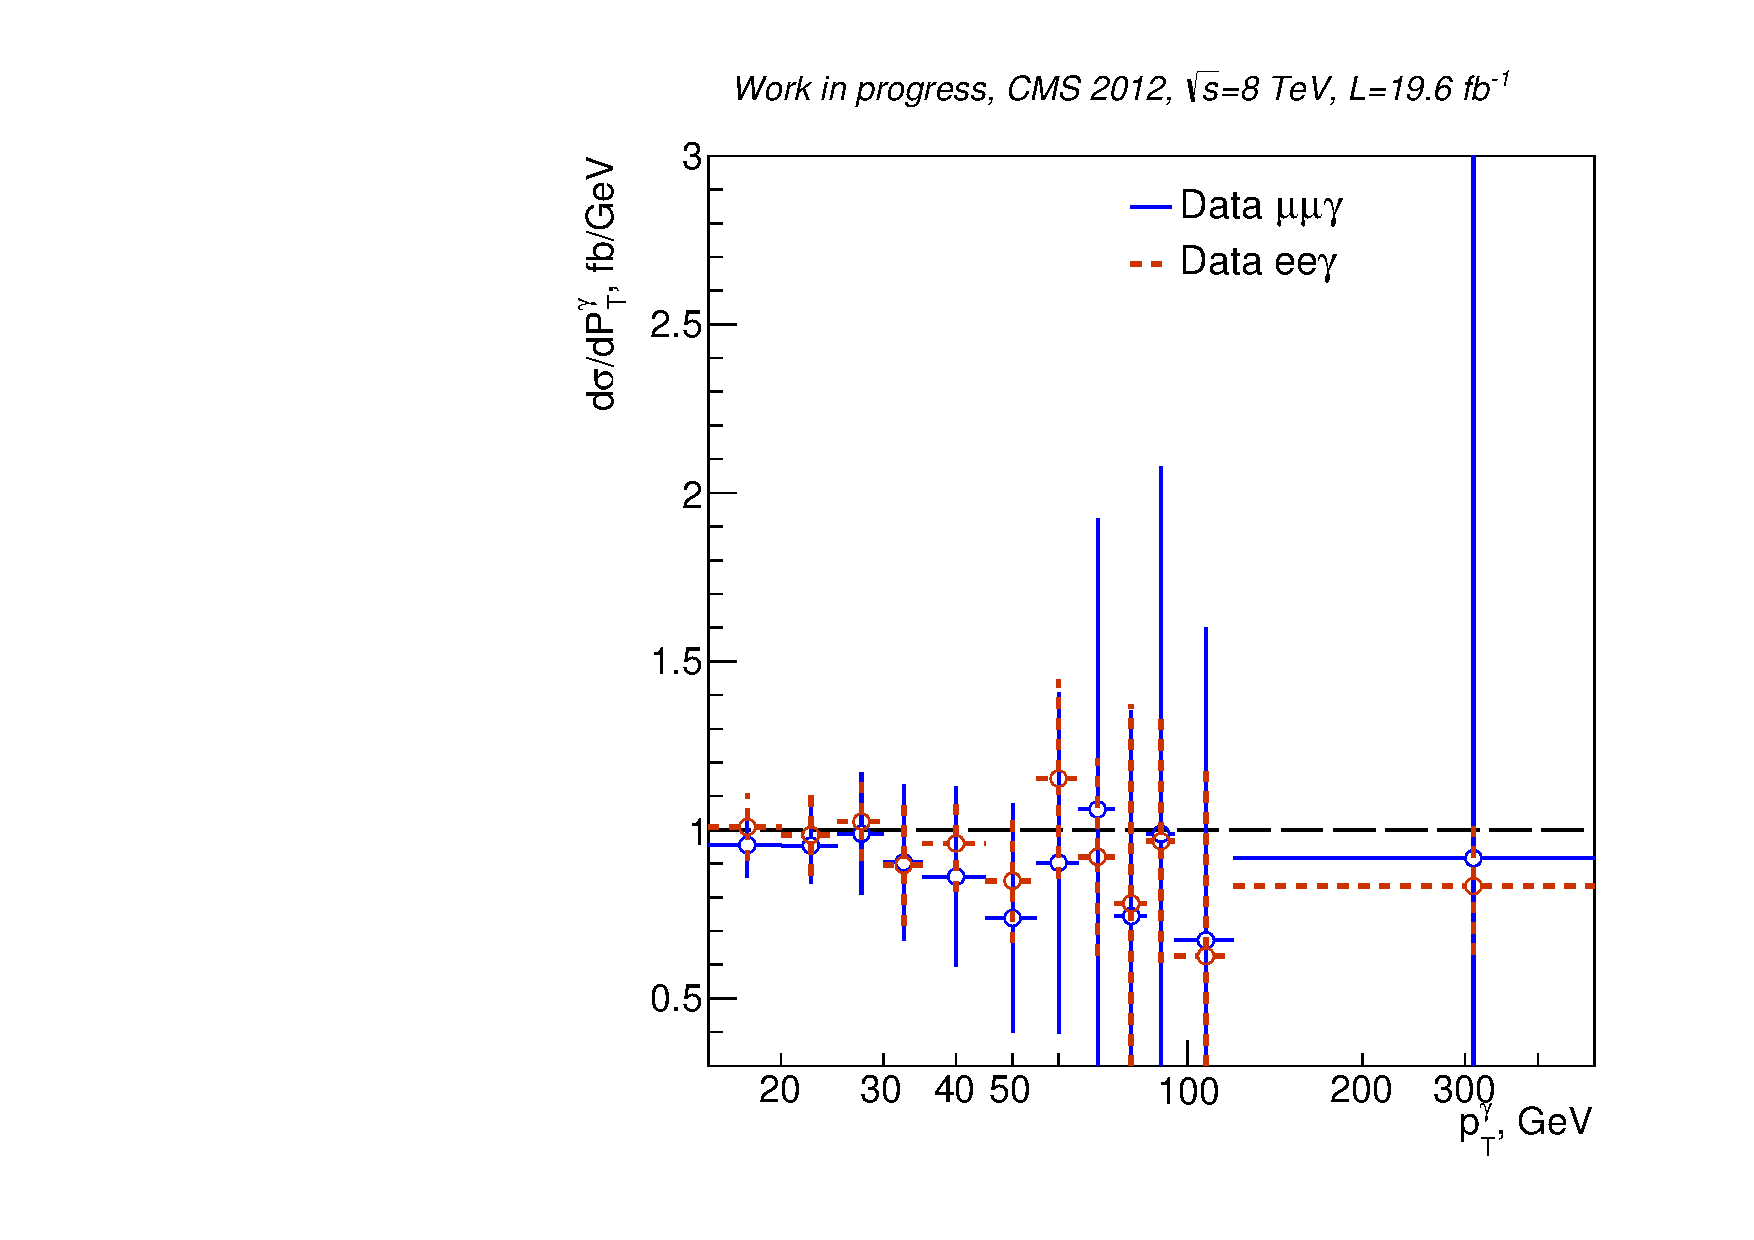
\includegraphics[width=0.33\textwidth]{../figs/figs_v11/ChannelsMERGED_ZGamma/CrossSection/compareCSratioOttoZGamma.pdf}
      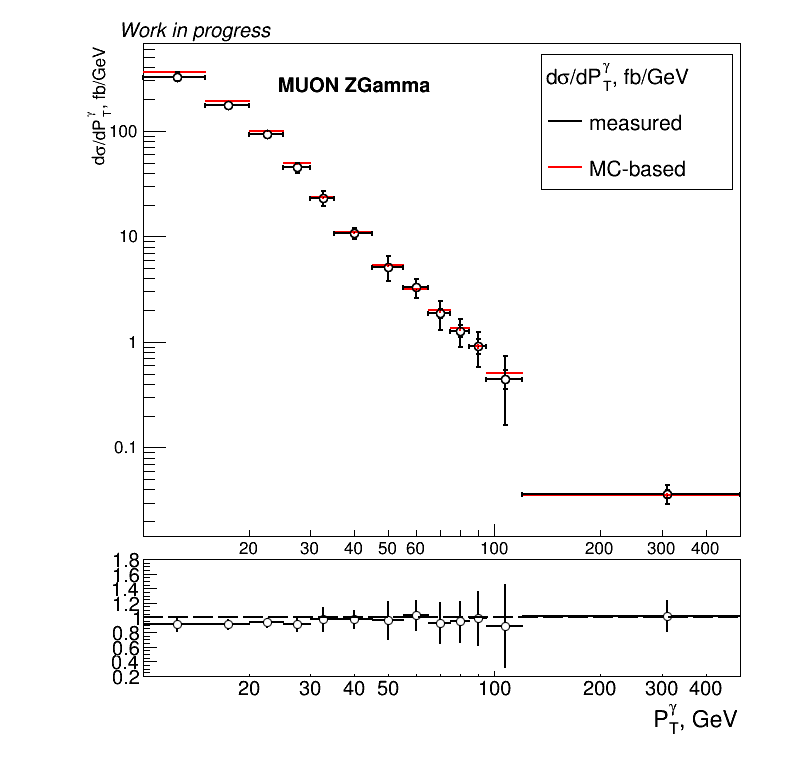
\includegraphics[width=0.48\textwidth]{../figs/figs_v11/MUON_ZGamma/CrossSection/c_CS_MUON_ZGamma_UNblind.png} 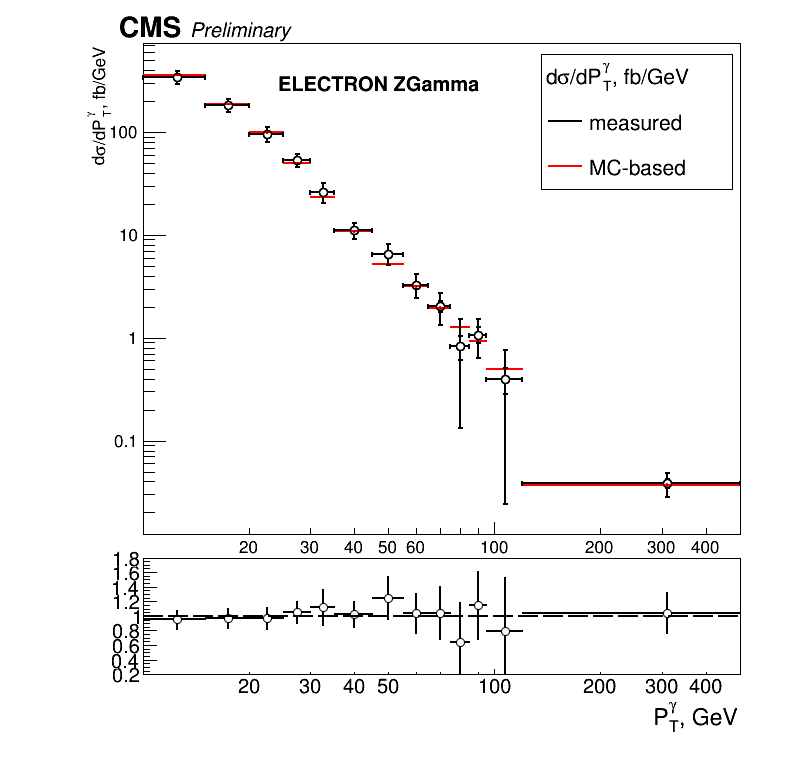
\includegraphics[width=0.48\textwidth]{../figs/figs_v11/ELECTRON_ZGamma/CrossSection/c_CS_ELECTRON_ZGamma_UNblind.png}
  \caption{$Z\gamma$ differential cross section. Top, left to right: the $Z\gamma$ differential cross section; the ratio of measured over the MC-based $Z\gamma$ differntial cross section; the ratio of the measured over published $Z\gamma$ differential cross section. Bottom:  the $Z\gamma$ measured differential cross section overlaid with the MC-based cross section, the muon channel (left) and the electron channel (right).}
  \label{fig:CS_Zg}
 \end{center}
\end{figure}
  

\begin{table}[h]
  \scriptsize
  \begin{center}
  \caption{Cross section and errors. MUON $Z\gamma$}
  \begin{tabular}{|c|c|c|}
    bin & $d\sigma/dP_{T}$ &$d\sigma/dP_{T}$ \\ 
    lims & MC based &    meas.       \\ \hline
    total & 2085 & $1985 \pm 18 \pm 62$ \\ \hline
%    10-15 & 360 & $323 \pm 5 \pm 17$ \\ \hline
    15-20 & 191 & $178 \pm 3 \pm 8$ \\ \hline
    20-25 & 100 & $98 \pm 2 \pm 5$ \\ \hline
    25-30 & 49 & $43 \pm 1 \pm 3$ \\ \hline
    30-35 & 24 & $23 \pm 1 \pm 2$ \\ \hline
    35-45 & 11 & $11 \pm 0 \pm 1$ \\ \hline
    45-55 & 5.3 & $5.2 \pm 0.3 \pm 0.7$ \\ \hline
    55-65 & 3.2 & $3.4 \pm 0.2 \pm 0.4$ \\ \hline
    65-75 & 2.0 & $2.1 \pm 0.2 \pm 0.3$ \\ \hline
    75-85 & 1.3 & $1.5 \pm 0.1 \pm 0.2$ \\ \hline
    85-95 & 0.9 & $1.1 \pm 0.1 \pm 0.2$ \\ \hline
    95-120 & 0.50 & $0.56 \pm 0.06 \pm 0.10$ \\ \hline
    120-500 & 0.036 & $0.040 \pm 0.003 \pm 0.006$ \\ \hline
  \end{tabular}
  \label{tab:sc_mc_vs_meas_MUON_ZGamma}
  \end{center}
\end{table}

\begin{table}[h]
  \scriptsize
  \begin{center}
  \caption{Cross section and errors. ELECTRON $Z\gamma$}
  \begin{tabular}{|c|c|c|}
    bin & $d\sigma/dP_{T}$ &$d\sigma/dP_{T}$ \\ 
    lims & MC based &    meas.       \\ \hline
    total & 2061 & $2091 \pm 24 \pm 70$ \\ \hline
%    10-15 & 357 & $350 \pm 6 \pm 17$ \\ \hline
    15-20 & 188 & $180 \pm 4 \pm 9$ \\ \hline
    20-25 & 99 & $101 \pm 3 \pm 6$ \\ \hline
    25-30 & 50 & $51 \pm 2 \pm 4$ \\ \hline
    30-35 & 23 & $25 \pm 1 \pm 2$ \\ \hline
    35-45 & 11 & $12 \pm 1 \pm 1$ \\ \hline
    45-55 & 5.2 & $6.5 \pm 0.4 \pm 0.7$ \\ \hline
    55-65 & 3.2 & $3.3 \pm 0.3 \pm 0.5$ \\ \hline
    65-75 & 1.9 & $2.3 \pm 0.2 \pm 0.4$ \\ \hline
    75-85 & 1.3 & $1.2 \pm 0.2 \pm 0.3$ \\ \hline
    85-95 & 0.9 & $1.1 \pm 0.2 \pm 0.3$ \\ \hline
    95-120 & 0.50 & $0.66 \pm 0.07 \pm 0.11$ \\ \hline
    120-500 & 0.037 & $0.042 \pm 0.004 \pm 0.006$ \\ \hline
  \end{tabular}
  \label{tab:sc_mc_vs_meas_ELECTRON_ZGamma}
  \end{center}
\end{table}

